\documentclass[a4paper,12pt]{article}
\usepackage{graphicx}
\usepackage{amsmath}
\usepackage{siunitx}
\sisetup{per-mode=symbol,exponent-product=\cdot,range-phrase=\ldots}
\usepackage{tikz,pgfplots}
\pgfplotsset{compat=1.18}
\usepackage{titlesec}
\usepackage{enumitem}
\usepackage{tex/ET_Ueb_Header_2Ebenen}
\graphicspath{{./}{./templates/}{./fig/}}
\renewcommand\thesection{\Alph{section}}
\titleformat{\section}[hang]{\normalfont\Large\bfseries}{Aufgabe \thesection)}{.8em}{}
\renewcommand\thesubsection{\thesection.\arabic{subsection}}
\titleformat{\subsection}[hang]{\normalfont\large\bfseries}{\thesubsection}{.8em}{}
\setlist[enumerate,1]{label=\thesubsection),ref=\thesubsection)}
\let\cpx\underline
\let\peak\hat
\newcommand\pcpx[1]{\peak{\cpx{#1}}}
\let\avg\overline
\newcommand{\abs}[1]{\left\lvert#1\right\rvert}
\newcommand{\dd}{\;\mathrm{d}}
\renewcommand{\d}{\operatorname{d}\!}
\renewcommand{\j}{\operatorname{j}\!}
\newcommand{\conj}[1]{{#1}^\ast}
\newcommand{\mat}[1]{\mathbf{#1}}
\newcommand{\cmat}[1]{\mat{\cpx{#1}}}
\makeatletter
\@ifundefined{Header}{\let\Header\makeheader}{}
\makeatother
\begin{document}
\begin{titlepage}
\thispagestyle{firstpage}
\vspace*{4cm}
\begin{center}
{\Large\bfseries Netzwerke und Schaltungen II, D-ITET\par}
\vspace{3mm}
{\Huge\bfseries Bodeplots — Musterlösung\par}
\vspace{9mm}
\end{center}
\vfill
\begingroup\footnotesize
\textbf{Hinweise}\\[2pt]
– Phasenverläufe können aus ästhetischen Gründen um $360^\circ$ verschoben sein; eine Verschiebung um $360^\circ$ ändert die Aussage nicht.\\
– Magnitudenplots sind auf der $y$-Achse standardmäßig in 20-dB-Schritten beschriftet; falls es sich ästhetisch anbietet, sind auch 10-dB-Schritte zulässig.\\
– Mit dem MATLAB-Skript kann man selbst experimentieren, die Plots exakt berechnen und alle Ergebnisse nachprüfen.\\
– Die Teilaufgaben a, b, g, h und p  sind ausführlicher erklärt als die übrigen.
\endgroup
\vfill
\end{titlepage}
\section*{Einleitung: \(s\) und \(j\omega\)}

Für sinusförmige stationäre Signale fällt die Laplace- mit der Fourier-Transfor- mierten auf der imaginären Achse zusammen; eine Abklinghülle ist nicht nötig, daher setzt man \(\sigma=0\) und damit
\[ s = j\omega. \]
Der Frequenzgang wird zwar als \(H(j\omega)\) ausgewertet, aber die Schreibweise in \(s\) ist kompakter: Standardformen wie \(1+sT\), \(1/(1+sT)\), \(sL\), \(1/(sC)\) sind sofort lesbar und direkt faktorisierbar. Vorgehen: in \(s\) modellieren und faktorisieren, um Magnituden/Phasen explitizit auszurechnen, am Ende \(s\to j\omega\) einsetzen.


\subsection*{Beispiele}

$$ H(s)=\frac{1}{1+sT}\qquad\Rightarrow\qquad H(j\omega)=\frac{1}{1+j\omega T} $$

$$ H(s)=\frac{sT}{1+sT}\qquad\Rightarrow\qquad H(j\omega)=\frac{j\omega T}{1+j\omega T} $$

$$ H(s)=\frac{1}{sT}\qquad\Rightarrow\qquad H(j\omega)=\frac{1}{j\omega T} $$

$$ H(s)=sT\qquad\Rightarrow\qquad H(j\omega)=j\omega T $$

$$ H(s)=\frac{\omega_0^2}{s^2+2\zeta \omega_0 s+\omega_0^2}\qquad\Rightarrow\qquad H(j\omega)=\frac{\omega_0^2}{-\omega^2+j\,2\zeta \omega_0 \omega+\omega_0^2} $$

$$ H(s)=\frac{1+sT_{z}}{1+sT_{p}}\qquad\Rightarrow\qquad H(j\omega)=\frac{1+j\omega T_{z}}{1+j\omega T_{p}} $$

\newpage
\section{}
\[
H(s)=\frac{1}{s+1}\,.
\]
\subsection{Bode-Diagramm}
\begin{center}
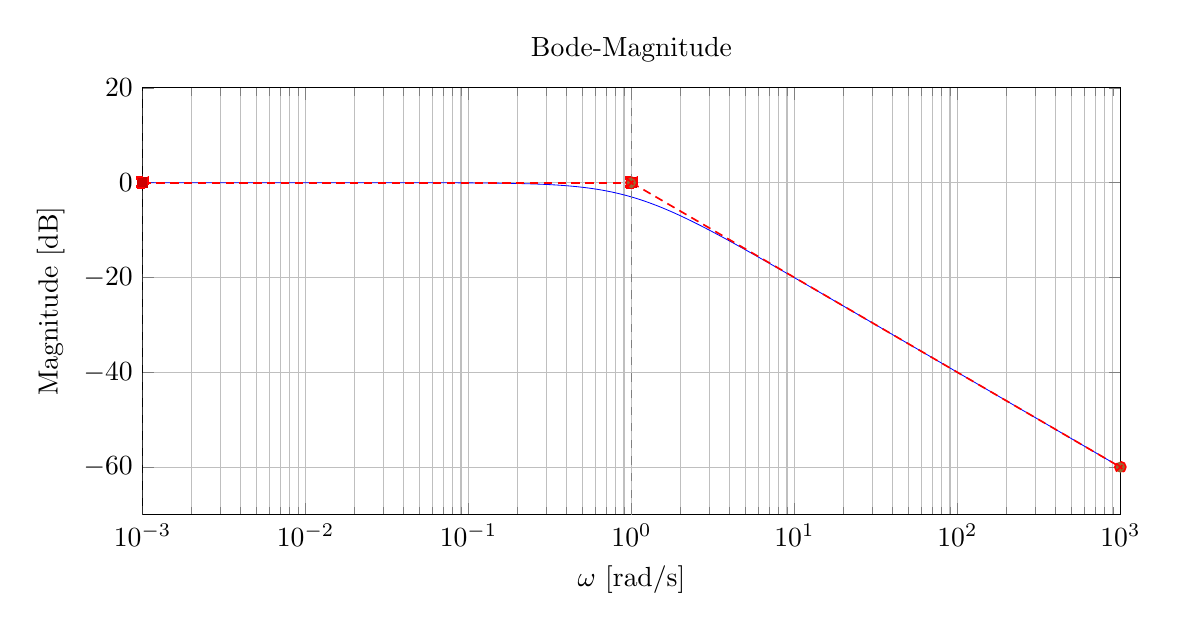
\begin{tikzpicture}
\begin{semilogxaxis}[
  width=14cm,height=7cm,
  ymin=-70,ymax=20,
  xmin=1e-3,xmax=1e3,
  xlabel={$\omega$ [rad/s]},
  ylabel={Magnitude [dB]},
  grid=both,
  title={Bode-Magnitude}
]
\addplot[
  domain=1e-3:1e3,
  samples=600,
  mark=none,
  line width=0.3pt,
  blue
] {-20*ln(sqrt(1 + x^2))/ln(10)};
\addplot+[domain=1e-3:1,samples=2,dashed,dash pattern=on 3pt off 2pt,line width=0.6pt,red] {0};
\addplot+[domain=1:1e3,samples=2,dashed,dash pattern=on 3pt off 2pt,line width=0.6pt,red] {-20*ln(x)/ln(10)};
\draw[gray,dashed] (rel axis cs:0,0) -- (rel axis cs:0,1);
\draw[gray,dashed] (axis cs:1,\pgfkeysvalueof{/pgfplots/ymin}) -- (axis cs:1,\pgfkeysvalueof{/pgfplots/ymax});
\node[gray,anchor=south east] at (axis cs:1,\pgfkeysvalueof{/pgfplots/ymax}) {\scriptsize Pol $\omega_p=1$};
\end{semilogxaxis}
\end{tikzpicture}
\vspace{6mm}
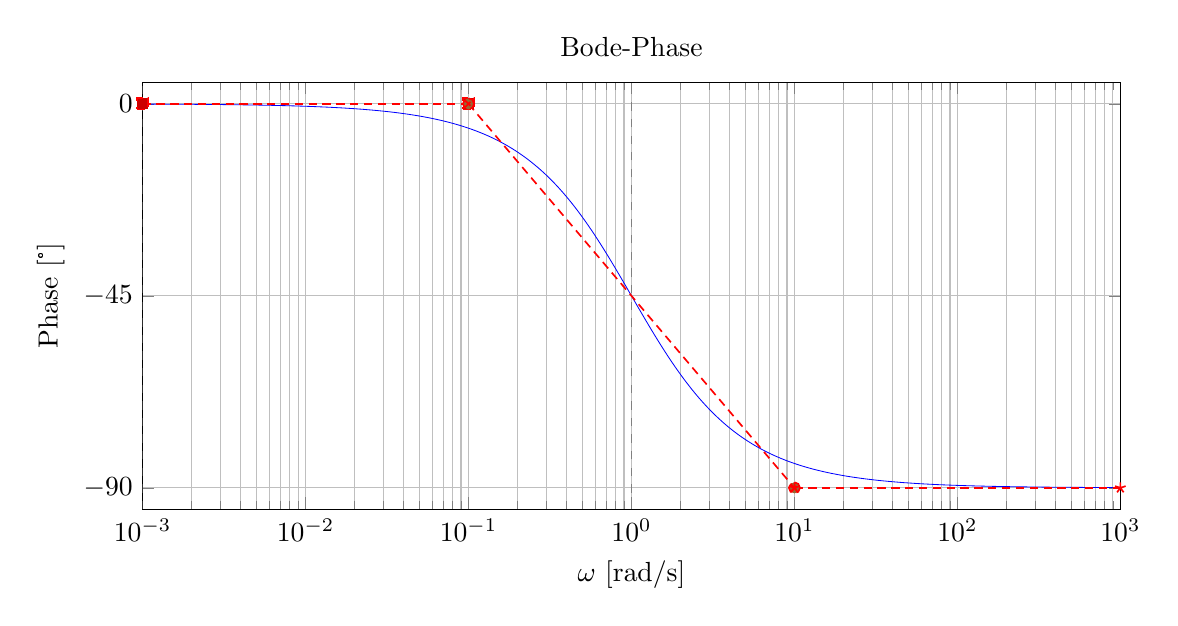
\begin{tikzpicture}
\begin{semilogxaxis}[
  width=14cm,height=7cm,
  xmin=1e-3,xmax=1e3,
  ymin=-95,ymax=5,
  ytick distance=45,
  xlabel={$\omega$ [rad/s]},
  ylabel={Phase [°]},
  grid=both,
  title={Bode-Phase}
]
\addplot[
  domain=1e-3:1e3,
  samples=600,
  mark=none,
  line width=0.3pt,
  blue
] {-atan(x)};
\addplot+[domain=1e-3:1e-1,samples=2,dashed,dash pattern=on 3pt off 2pt,line width=0.6pt,red] {0};
\addplot+[domain=1e-1:1e1,samples=2,dashed,dash pattern=on 3pt off 2pt,line width=0.6pt,red] {-45 - 45*ln(x)/ln(10)};
\addplot+[domain=1e1:1e3,samples=2,dashed,dash pattern=on 3pt off 2pt,line width=0.6pt,red] {-90};
\draw[gray,dashed] (rel axis cs:0,0) -- (rel axis cs:0,1);
\draw[gray,dashed] (axis cs:1,\pgfkeysvalueof{/pgfplots/ymin}) -- (axis cs:1,\pgfkeysvalueof{/pgfplots/ymax});
\node[gray,anchor=south east] at (axis cs:1,\pgfkeysvalueof{/pgfplots/ymax}) {\scriptsize Pol $\omega_p=1$};
\end{semilogxaxis}
\end{tikzpicture}
\end{center}

\subsection{Erklärung}
\begin{description}[leftmargin=1.2em,labelsep=.6em,font=\bfseries]

\item[1. Normalform herstellen.]
Bringe die Übertragungsfunktion exakt in die im Skript definierte Standardform für reelle Pol-/Nullstellen.
\[
H(s)=\frac{1}{1+sT_p}\quad\text{mit}\quad T_p=1.
\]
Hier haben wir: \[
\underline{F}_1(s)=\frac{1}{1+sT_p}\quad\text{und}\quad K_0 = 1\quad \text{und}\quad r = 0.
\]
Klassifizikation des ersten Teilglieds $\underline{F}_1$: reelles Polglied erster Ordnung.

\item[2. Eckfrequenz bestimmen und sortieren.]
Bestimme die Eckfrequenz aus der Zeitkonstante:
\[
\omega_p=\frac{1}{T_p}=1\,\mathrm{rad/s}.
\]
Es existiert nur diese Eckfrequenz; die aufsteigende Sortierung \(\omega_1<\omega_2<\dots\) ist damit trivial. 

\item[3. Startpunkt des Amplitudengangs festlegen (Geradennäherung).]
Setze die Startfrequenz gleich der kleinsten Eckfrequenz \(\omega_{\min}=\omega_p = 1\,\mathrm{rad/s}\). Verwende die Skript-Regel
\[
F_{\mathrm{dB}}(\omega_{\min})=20\log_{10}\!\Big(|K_0\,F^*_{ges}(0)|\cdot\,\omega_{\min}^{\,r}\Big) = 20 \log_{10}(1) = 0\,\mathrm{dB}
\]
Hier gilt \(K_0=1\), \(r=0\) und \(F^*_{ges}(0)=1\Rightarrow F_{\mathrm{dB}}(\omega_{\min})=0\,\mathrm{dB}\). Dieser Punkt nützt uns als Anker für die Geradennäherung. 

\item[4. Verlauf links vom Startpunkt zeichnen.]
Für \(\omega<\omega_{\min}\) bleibt die Amplituden-Asymptote waagrecht, denn die Anfangssteigung beträgt \(r\cdot 20\,\mathrm{dB/dec}=0\). Trage also eine horizontale Linie bei \(0\,\mathrm{dB}\) ein. 

\item[5. Steigungswechsel an der Eckfrequenz eintragen.]
Ein einfaches Polglied \(1/(1+sT_p)\) reduziert die Steigung ab \(\omega_p\) um \(20\,\mathrm{dB/dec}\). Da bist jetzt die Steigung \(0\,\mathrm{dB/dec}\) betrug, ist diese ab jetzt \(-20\,\mathrm{dB/dec}\). Zeichne rechts von \(\omega_p\) die Gerade mit Steigung \(-20\,\mathrm{dB/dec}\). Die Formel für die Geradennäherung lautet:
\[
|H(j\omega)|_{\mathrm{dB}}\approx -20\log_{10}\omega\quad(\omega\ge 1).
\]
Mehrfachpole würden die Änderung mehrfach zählen; hier nicht nötig. 

\item[6. Eckabrundung korrekt berücksichtigen.]
Bei einfachen reellen Polen ergibt sich am Knickpunkt \(\omega=\omega_p\) eine Abweichung von \(-3\,\mathrm{dB}\) gegenüber der Gerade. Setze dort einen Stützpunkt:
\[
|H(j\omega_p)|_{\mathrm{dB}}=-10\log_{10}(1+1^2)=-10\log_{10}2\approx -3.01\,\mathrm{dB}.
\]
Runde die Ecke entsprechend ab. Hätten wir einen Mehrfachpol bei \(\omega_p\) (Beispielsweise \(\big(\frac{1}{1+sT_p}\big)^t\)), müsste man die Ecke um \(t \cdot 3.01\, \mathrm{dB}\) abrunden.  

\item[7. Phasenstartwert festlegen.]
Nutze die Regel für \(\omega\to 0\): Da \(K_0F_{ges}(0)>0\) und \(r=0\), ist der Startwert der Phase
\[
\varphi(0)=0^\circ.
\]


\item[8. Phasenänderung durch das Polglied eintragen.]
Ein reelles Polglied erster Ordnung erzeugt insgesamt eine Phasenänderung von \(-90^\circ\). Trage die Näherung ein:
\[
\varphi(\omega)\approx
\begin{cases}
0^\circ,& \omega\le 0.1\,\omega_p,\\
\text{linear mit Steigung }-45^\circ/\text{Dec},& 0.1\,\omega_p<\omega<10\,\omega_p,\\
-90^\circ,& \omega\ge 10\,\omega_p.
\end{cases}
\]
Das lineare Zwischenstück kann Formelkonform als \(\varphi(\omega)\approx -45^\circ-45^\circ\log_{10}\omega\) dargestellt werden (hier mit \(\omega_p=1\)). 

\item[9. Grenzwerte und Konsistenz prüfen.]
DC: \(|H(0)|=1\Rightarrow 0\,\mathrm{dB}\), \(\varphi(0)=0^\circ\). HF: \(|H(j\omega)|\sim 1/\omega\Rightarrow -20\log_{10}\omega\,\mathrm{dB}\)). Pol-/Nullzählung bestätigt die Endphase: Zählergrad \(m=0\), Nennergra \(n=1\Rightarrow \varphi(\infty)=(m-n)\cdot 90^\circ=-90^\circ\). 

\end{description}

\subsubsection*{Stückweise Näherungen (für die Skizze)}
\[
|H(j\omega)|_{\mathrm{dB}}\approx
\begin{cases}
0,& \omega\ll 1,\\[2pt]
-10\log_{10}2,& \omega=1,\\[2pt]
-20\log_{10}\omega,& \omega\gg 1,
\end{cases}
\qquad
\varphi(\omega)\approx
\begin{cases}
0^\circ,& \omega\le 0.1,\\[2pt]
-45^\circ-45^\circ\log_{10}\omega,& 0.1<\omega<10,\\[2pt]
-90^\circ,& \omega\ge 10.
\end{cases}
\]

\newpage 
\section{}
\[
H(s)=\frac{10}{s+10}\,.
\]
\subsection{Bode-Diagramm}
\begin{center}
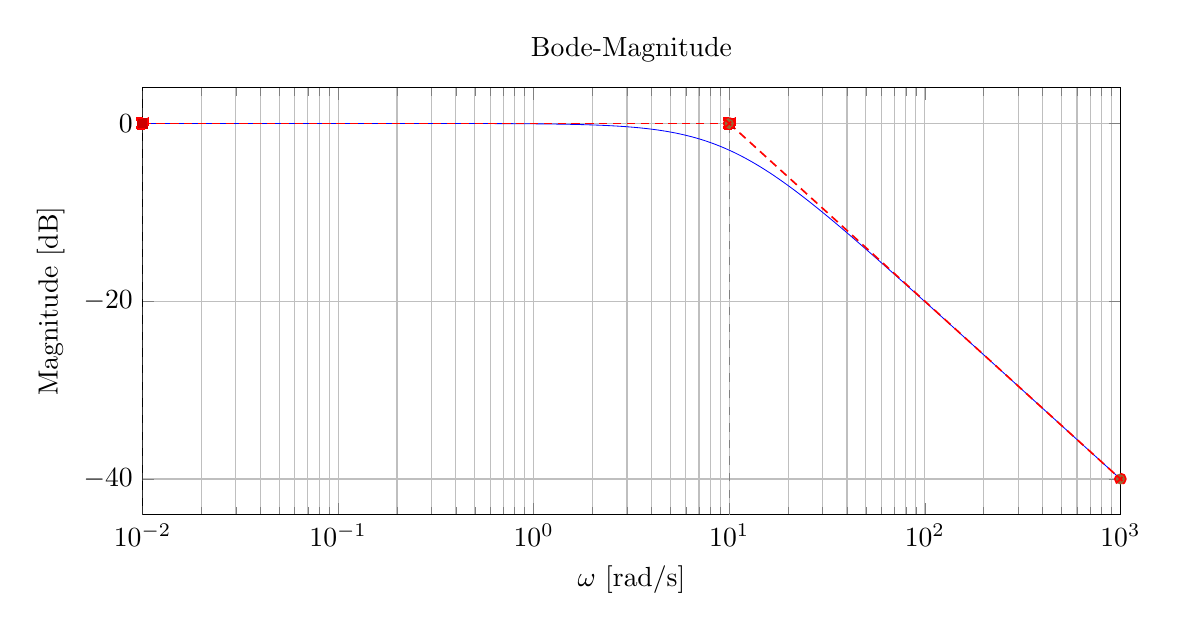
\begin{tikzpicture}
\begin{semilogxaxis}[
  width=14cm,height=7cm,
  xmin=1e-2,xmax=1e3,
  xlabel={$\omega$ [rad/s]},
  ylabel={Magnitude [dB]},
  grid=both,
  ytick distance=20, 
  title={Bode-Magnitude}
]
\addplot[
  domain=1e-2:1e3,
  samples=600,
  mark=none,
  line width=0.3pt,
  blue
] {-20*ln(sqrt(1 + (x/10)^2))/ln(10)};
\addplot+[domain=1e-2:1e1,samples=2,dashed,dash pattern=on 3pt off 2pt,line width=0.6pt,red] {0};
\addplot+[domain=1e1:1e3,samples=2,dashed,dash pattern=on 3pt off 2pt,line width=0.6pt,red] {-20*ln(x/10)/ln(10)};
\draw[gray,dashed] (rel axis cs:0,0) -- (rel axis cs:0,1);
\draw[gray,dashed] (axis cs:10,\pgfkeysvalueof{/pgfplots/ymin}) -- (axis cs:10,\pgfkeysvalueof{/pgfplots/ymax});
\node[gray,anchor=south east] at (axis cs:10,\pgfkeysvalueof{/pgfplots/ymax}) {\scriptsize Pol $\omega_p=10$};
\end{semilogxaxis}
\end{tikzpicture}
\vspace{6mm}
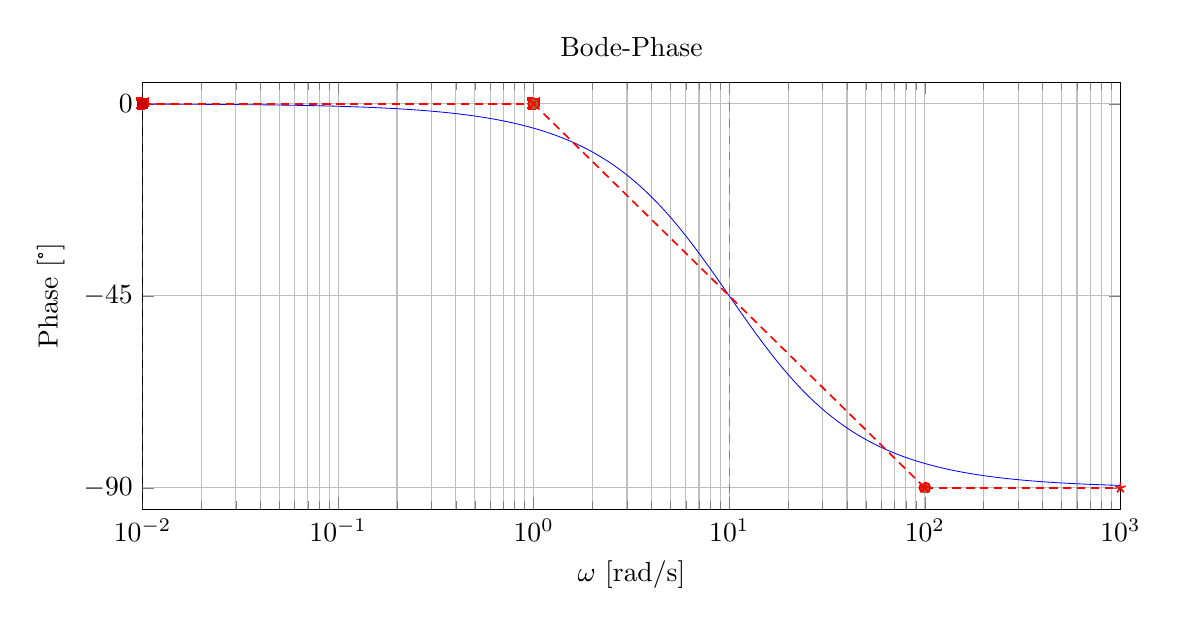
\begin{tikzpicture}
\begin{semilogxaxis}[
  width=14cm,height=7cm,
  xmin=1e-2,xmax=1e3,
  ytick distance=45,
  ymin=-95,ymax=5,
  xlabel={$\omega$ [rad/s]},
  ylabel={Phase [°]},
  grid=both,
  title={Bode-Phase}
]
\addplot[
  domain=1e-2:1e3,
  samples=600,
  mark=none,
  line width=0.3pt,
  blue
] {-atan(x/10)};
\addplot+[domain=1e-2:1e0,samples=2,dashed,dash pattern=on 3pt off 2pt,line width=0.6pt,red] {0};
\addplot+[domain=1e0:1e2,samples=2,dashed,dash pattern=on 3pt off 2pt,line width=0.6pt,red] {-45 - 45*ln(x/10)/ln(10)};
\addplot+[domain=1e2:1e3,samples=2,dashed,dash pattern=on 3pt off 2pt,line width=0.6pt,red] {-90};
\draw[gray,dashed] (rel axis cs:0,0) -- (rel axis cs:0,1);
\draw[gray,dashed] (axis cs:10,\pgfkeysvalueof{/pgfplots/ymin}) -- (axis cs:10,\pgfkeysvalueof{/pgfplots/ymax});
\node[gray,anchor=south east] at (axis cs:10,\pgfkeysvalueof{/pgfplots/ymax}) {\scriptsize Pol $\omega_p=10$};
\end{semilogxaxis}
\end{tikzpicture}
\end{center}
\newpage
\subsection{Erklärung (ausführlich)}
\begin{description}[leftmargin=1.2em,labelsep=.6em,font=\bfseries]

\item[1. Normalform herstellen.]
Bringe die Übertragungsfunktion exakt in die im Skript definierte Standardform für reelle Pol-/Nullstellen.
\[
H(s)=\frac{1}{1+sT_p}\quad\text{mit}\quad T_p=\frac{1}{10}.
\]
Hier haben wir: \[
\underline{F}_1(s)=\frac{1}{1+sT_p}\quad\text{und}\quad K_0 = 1\quad \text{und}\quad r = 0.
\]
Klassifizikation des ersten Teilglieds $\underline{F}_1$: reelles Polglied (LHP) erster Ordnung.

\item[2. Eckfrequenz bestimmen und sortieren.]
Bestimme die Eckfrequenz aus der Zeitkonstante:
\[
\omega_p=\frac{1}{T_p}=10\,\mathrm{rad/s}.
\]
Es existiert nur diese Eckfrequenz; die aufsteigende Sortierung \(\omega_1<\omega_2<\dots\) ist damit trivial. 

\item[3. Startpunkt des Amplitudengangs festlegen (Geradennäherung).]
Setze die Startfrequenz gleich der kleinsten Eckfrequenz \(\omega_{\min}=\omega_p = 10\,\mathrm{rad/s}\). Verwende die Skript-Regel
\[
F_{\mathrm{dB}}(\omega_{\min})=20\log_{10}\!\Big(|K_0\,F^*_{ges}(0)|\cdot\,\omega_{\min}^{\,r}\Big) = 20 \log_{10}(1) = 0\,\mathrm{dB}.
\]
Hier gilt \(K_0=1\), \(r=0\) und \(F^*_{ges}(0)=1\Rightarrow F_{\mathrm{dB}}(\omega_{\min})=0\,\mathrm{dB}\). Dieser Punkt nützt uns als Anker für die Geradennäherung. 

\item[4. Verlauf links vom Startpunkt zeichnen.]
Für \(\omega<\omega_{\min}\) bleibt die Amplituden-Asymptote waagrecht, denn die Anfangssteigung beträgt \(r\cdot 20\,\mathrm{dB/dec}=0\). Trage also eine horizontale Linie bei \(0\,\mathrm{dB}\) ein. 

\item[5. Steigungswechsel an der Eckfrequenz eintragen.]
Ein einfaches Polglied \(1/(1+sT_p)\) reduziert die Steigung ab \(\omega_p\) um \(20\,\mathrm{dB/dec}\). Da bis jetzt die Steigung \(0\,\mathrm{dB/dec}\) betrug, ist diese ab jetzt \(-20\,\mathrm{dB/dec}\). Zeichne rechts von \(\omega_p\) die Gerade mit Steigung \(-20\,\mathrm{dB/dec}\). Die Formel für die Geradennäherung lautet:
\[
|H(j\omega)|_{\mathrm{dB}}\approx -20\log_{10}\!\Big(\frac{\omega}{10}\Big)\quad(\omega\ge 10).
\]
Mehrfachpole würden die Änderung mehrfach zählen; hier nicht nötig. 

\item[6. Eckabrundung korrekt berücksichtigen.]
Bei einfachen reellen Polen ergibt sich am Knickpunkt \(\omega=\omega_p\) eine Abweichung von \(-3\,\mathrm{dB}\) gegenüber der Gerade.
\item[7. Phasenstartwert festlegen.]
Nutze die Regel für \(\omega\to 0\): Da \(K_0F_{ges}(0)>0\) und \(r=0\), ist der Startwert der Phase
\[
\varphi(0)=r \cdot 90^\circ=0^\circ.
\]

\item[8. Phasenänderung durch das Polglied eintragen.]
Ein reelles Polglied erster Ordnung erzeugt insgesamt eine Phasenänderung von \(-90^\circ\). Trage die Näherung ein:
\[
\varphi(\omega)\approx
\begin{cases}
0^\circ,& \omega\le 0.1\,\omega_p\;(=1),\\
\text{linear mit Steigung }-45^\circ/\text{Dec},& 0.1\,\omega_p<\omega<10\,\omega_p\;(=100),\\
-90^\circ,& \omega\ge 10\,\omega_p\;(=100).
\end{cases}
\]
Das lineare Zwischenstück kann Formelkonform als \(\varphi(\omega)\approx -45^\circ-45^\circ\log_{10}(\omega/10)\) dargestellt werden (hier mit \(\omega_p=10\)). 

\item[9. Grenzwerte und Konsistenz prüfen.]
DC: \(|H(0)|=1\Rightarrow 0\,\mathrm{dB}\), \(\varphi(0)=0^\circ\). HF: \(|H(j\omega)|\sim 10/\omega\Rightarrow -20\log_{10}(\omega/10)\,\mathrm{dB}\)). Pol-/Nullzählung bestätigt die Endphase: Zählergrad \(m=0\), Nennergrad \(n=1\Rightarrow \varphi(\infty)=(m-n)\cdot 90^\circ=-90^\circ\). 

\end{description}

\subsubsection*{Stückweise Näherungen (für die Skizze)}
\[
|H(j\omega)|_{\mathrm{dB}}\approx
\begin{cases}
0,& \omega\ll 10,\\[2pt]
-10\log_{10}2,& \omega=10,\\[2pt]
-20\log_{10}(\omega/10),& \omega\gg 10,
\end{cases}
\]
\vspace{0.3cm}
\[
\varphi(\omega)\approx
\begin{cases}
0^\circ,& \omega\le 1,\\[2pt]
-45^\circ-45^\circ\log_{10}(\omega/10),& 1<\omega<100,\\[2pt]
-90^\circ,& \omega\ge 100.
\end{cases}
\]

\newpage
\section{}
\[
H(s)=\frac{s+1}{s+10}\,.
\]
\subsection{Bode-Diagramm}
\begin{center}
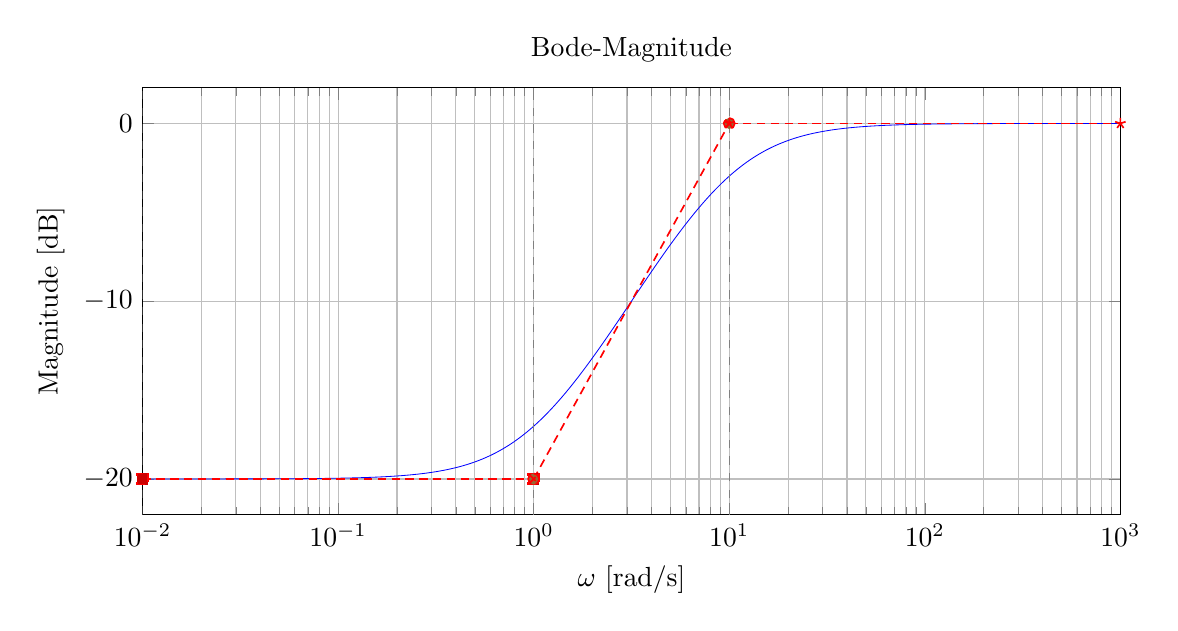
\begin{tikzpicture}
\begin{semilogxaxis}[
  width=14cm,height=7cm,
  xmin=1e-2,xmax=1e3,
  xlabel={$\omega$ [rad/s]},
  ylabel={Magnitude [dB]},
  grid=both,
  ytick distance=10,
  title={Bode-Magnitude}
]
\addplot[
  domain=1e-2:1e3,
  samples=600,
  mark=none,
  line width=0.3pt,
  blue
] {20*ln(sqrt(1 + x^2))/ln(10) - 20*ln(sqrt(100 + x^2))/ln(10)};
\addplot+[domain=1e-2:1,samples=2,dashed,dash pattern=on 3pt off 2pt,line width=0.6pt,red] {-20};
\addplot+[domain=1:1e1,samples=2,dashed,dash pattern=on 3pt off 2pt,line width=0.6pt,red] {-20 + 20*ln(x)/ln(10)};
\addplot+[domain=1e1:1e3,samples=2,dashed,dash pattern=on 3pt off 2pt,line width=0.6pt,red] {0};
\draw[gray,dashed] (rel axis cs:0,0) -- (rel axis cs:0,1);
\draw[gray,dashed] (axis cs:1,\pgfkeysvalueof{/pgfplots/ymin}) -- (axis cs:1,\pgfkeysvalueof{/pgfplots/ymax});
\draw[gray,dashed] (axis cs:10,\pgfkeysvalueof{/pgfplots/ymin}) -- (axis cs:10,\pgfkeysvalueof{/pgfplots/ymax});
\node[gray,anchor=south east] at (axis cs:1,\pgfkeysvalueof{/pgfplots/ymax}) {\scriptsize Nullstelle $\omega_z=1$};
\node[gray,anchor=south east] at (axis cs:10,\pgfkeysvalueof{/pgfplots/ymax}) {\scriptsize Pol $\omega_p=10$};
\end{semilogxaxis}
\end{tikzpicture}
\vspace{6mm}
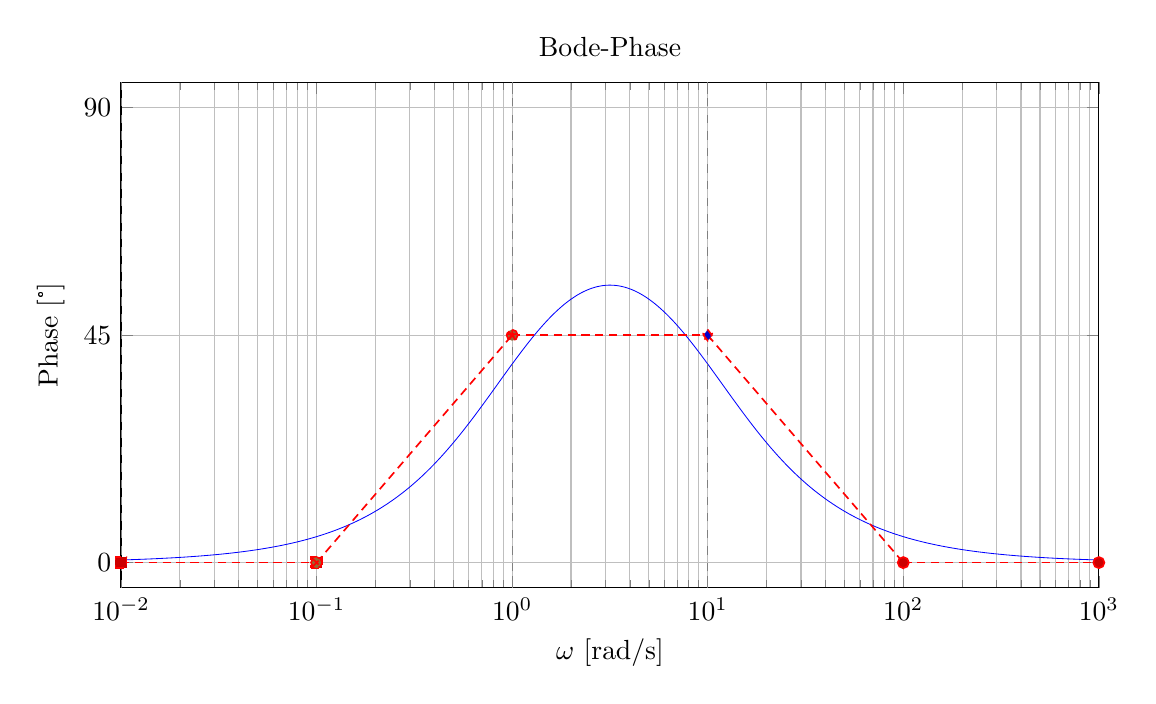
\begin{tikzpicture}
\begin{semilogxaxis}[
  width=14cm,height=8cm,
  xmin=1e-2,xmax=1e3,
  ymin=-5,ymax=95,
  ytick distance=45,
  xlabel={$\omega$ [rad/s]},
  ylabel={Phase [°]},
  grid=both,
  title={Bode-Phase}
]
\addplot[
  domain=1e-2:1e3,
  samples=600,
  mark=none,
  line width=0.3pt,
  blue
] {atan(x) - atan(x/10)};
\addplot+[domain=1e-2:1e-1,samples=2,dashed,dash pattern=on 3pt off 2pt,line width=0.6pt,red] {0};
\addplot+[domain=1e-1:1e0,samples=2,dashed,dash pattern=on 3pt off 2pt,line width=0.6pt,red] {45 + 45*ln(x)/ln(10)};
\addplot+[domain=1e0:1e1,samples=2,dashed,dash pattern=on 3pt off 2pt,line width=0.6pt,red] {45};
\addplot+[domain=1e1:1e2,samples=2,dashed,dash pattern=on 3pt off 2pt,line width=0.6pt,red] {45 - 45*ln(x/10)/ln(10)};
\addplot+[domain=1e2:1e3,samples=2,dashed,dash pattern=on 3pt off 2pt,line width=0.6pt,red] {0};
\draw[gray,dashed] (rel axis cs:0,0) -- (rel axis cs:0,1);
\draw[gray,dashed] (axis cs:1,\pgfkeysvalueof{/pgfplots/ymin}) -- (axis cs:1,\pgfkeysvalueof{/pgfplots/ymax});
\draw[gray,dashed] (axis cs:10,\pgfkeysvalueof{/pgfplots/ymin}) -- (axis cs:10,\pgfkeysvalueof{/pgfplots/ymax});
\node[gray,anchor=south east] at (axis cs:1,\pgfkeysvalueof{/pgfplots/ymax}) {\scriptsize Nullstelle $\omega_z=1$};
\node[gray,anchor=south east] at (axis cs:10,\pgfkeysvalueof{/pgfplots/ymax}) {\scriptsize Pol $\omega_p=10$};
\end{semilogxaxis}
\end{tikzpicture}
\end{center}
\newpage
\subsection{Erklärung}
\vspace{5mm}
\begin{description}[leftmargin=1.2em,labelsep=.6em,font=\bfseries]
\item[Schritt 1] DC-Faktor $\tfrac{1}{10}$: $H(s)=\tfrac{s+1}{s+10}=\tfrac{1+s}{10(1+s/10)}$. Für $\omega\ll1$ dominiert der DC-Anteil: $|H(\j\omega)|\approx\tfrac{1}{10}$, daher Betrag $-20\,\mathrm{dB}$ ohne Startsteigung; Startphase $\approx0^\circ$.
\item[Schritt 2] Nullstelle bei $\omega_z=1\,\mathrm{rad/s}$: ab $\omega=1$ steigt die Magnitude mit $+20\,\mathrm{dB/dec}$; zwischen $\omega_l=0.1$ und $\omega_h=10$ wächst die Phasenbeitrag der Nullstelle näherungsweise linear von $0^\circ$ auf $+90^\circ$ (Geradennäherung: $+45^\circ+45\log_{10}\omega$ in $[0.1,10]$), sodass bei $\omega=1$ etwa $+45^\circ$ erreicht werden.
\item[Schritt 3] Pol bei $\omega_p=10\,\mathrm{rad/s}$: ab $\omega=10$ kommt ein Steigungswechsel von $-20\,\mathrm{dB/dec}$ hinzu; dadurch wird die Gesamtslope wieder $0\,\mathrm{dB/dec}$ und der Betrag konvergiert gegen $0\,\mathrm{dB}$ für $\omega\gg10$. Der Pol führt in $[1,100]$ zu einer Phasenabnahme um $90^\circ$ (Geradennäherung: $+45^\circ-45\log_{10}(\omega/10)$), sodass die Gesamtphase für $\omega\gg100$ wieder gegen $0^\circ$ fällt. Das Zwischenband $1\le\omega\le10$ ist somit nahezu phasenflach bei $\approx+45^\circ$ und weist eine Betrags-Slope von $+20\,\mathrm{dB/dec}$ auf.
\end{description}

\vspace{0.5cm}
\medskip
\noindent\textbf{Stückweise Näherung}
\[
|H(\j\omega)|_{\mathrm{dB}}\approx
\begin{cases}
-20,& \omega\ll1,\\[4pt]
-20+20\log_{10}\omega,& 1\ll\omega\ll10,\\[4pt]
0,& \omega\gg10,
\end{cases}
\qquad
\]
\newpage
\section{}
\[
H(s)=\frac{10\,(1 - s)}{s+10}\,.
\]
\subsection{Bode-Diagramm}
\begin{center}
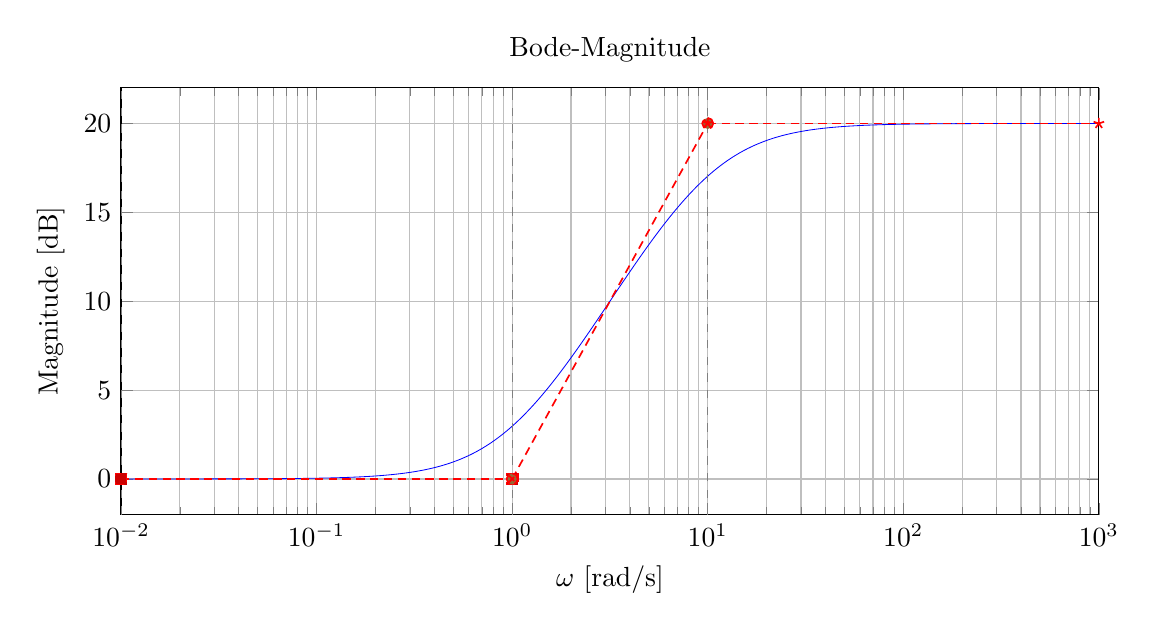
\begin{tikzpicture}
\begin{semilogxaxis}[
  width=14cm,height=7cm,
  xmin=1e-2,xmax=1e3,
  xlabel={$\omega$ [rad/s]},
  ylabel={Magnitude [dB]},
  grid=both,
  title={Bode-Magnitude}
]
\addplot[
  domain=1e-2:1e3,
  samples=600,
  mark=none,
  ytick distance=10,
  line width=0.3pt,
  blue
] {20 + 20*ln(sqrt(1 + x^2))/ln(10) - 20*ln(sqrt(100 + x^2))/ln(10)};
\addplot+[domain=1e-2:1,samples=2,dashed,dash pattern=on 3pt off 2pt,line width=0.6pt,red] {0};
\addplot+[domain=1:1e1,samples=2,dashed,dash pattern=on 3pt off 2pt,line width=0.6pt,red] {20*ln(x)/ln(10)};
\addplot+[domain=1e1:1e3,samples=2,dashed,dash pattern=on 3pt off 2pt,line width=0.6pt,red] {20};
\draw[gray,dashed] (rel axis cs:0,0) -- (rel axis cs:0,1);
\draw[gray,dashed] (axis cs:1,\pgfkeysvalueof{/pgfplots/ymin}) -- (axis cs:1,\pgfkeysvalueof{/pgfplots/ymax});
\draw[gray,dashed] (axis cs:10,\pgfkeysvalueof{/pgfplots/ymin}) -- (axis cs:10,\pgfkeysvalueof{/pgfplots/ymax});
\node[gray,anchor=south east] at (axis cs:1,\pgfkeysvalueof{/pgfplots/ymax}) {\scriptsize Nullstelle $\omega_z=1$ (RHP)};
\node[gray,anchor=south east] at (axis cs:10,\pgfkeysvalueof{/pgfplots/ymax}) {\scriptsize Pol $\omega_p=10$};
\end{semilogxaxis}
\end{tikzpicture}
\vspace{6mm}
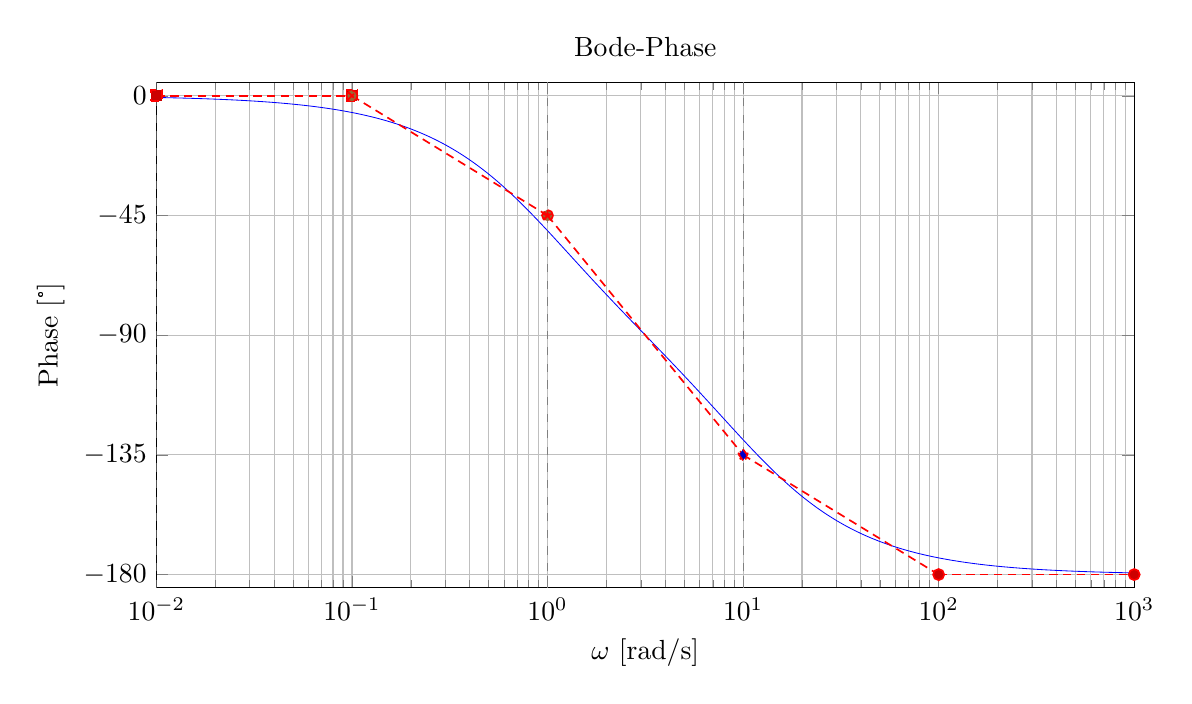
\begin{tikzpicture}
\begin{semilogxaxis}[
  width=14cm,height=8cm,
  xmin=1e-2,xmax=1e3,
  ymin=-185,ymax=5,
  xlabel={$\omega$ [rad/s]},
  ylabel={Phase [°]},
  ytick distance=45,
  grid=both,
  title={Bode-Phase}
]
\addplot[
  domain=1e-2:1e3,
  samples=600,
  mark=none,
  line width=0.3pt,
  blue
] {-atan(x) - atan(x/10)};
\addplot+[domain=1e-2:1e-1,samples=2,dashed,dash pattern=on 3pt off 2pt,line width=0.6pt,red] {0};
\addplot+[domain=1e-1:1e0,samples=2,dashed,dash pattern=on 3pt off 2pt,line width=0.6pt,red] {-45 - 45*ln(x)/ln(10)};
\addplot+[domain=1e0:1e1,samples=2,dashed,dash pattern=on 3pt off 2pt,line width=0.6pt,red]{-45 - 90*ln(x)/ln(10)};
\addplot+[domain=1e1:1e2,samples=2,dashed,dash pattern=on 3pt off 2pt,line width=0.6pt,red] {-135 - 45*ln(x/10)/ln(10)};
\addplot+[domain=1e2:1e3,samples=2,dashed,dash pattern=on 3pt off 2pt,line width=0.6pt,red] {-180};
\draw[gray,dashed] (rel axis cs:0,0) -- (rel axis cs:0,1);
\draw[gray,dashed] (axis cs:1,\pgfkeysvalueof{/pgfplots/ymin}) -- (axis cs:1,\pgfkeysvalueof{/pgfplots/ymax});
\draw[gray,dashed] (axis cs:10,\pgfkeysvalueof{/pgfplots/ymin}) -- (axis cs:10,\pgfkeysvalueof{/pgfplots/ymax});
\node[gray,anchor=south east] at (axis cs:1,\pgfkeysvalueof{/pgfplots/ymax}) {\scriptsize Nullstelle $\omega_z=1$ (RHP)};
\node[gray,anchor=south east] at (axis cs:10,\pgfkeysvalueof{/pgfplots/ymax}) {\scriptsize Pol $\omega_p=10$};
\end{semilogxaxis}
\end{tikzpicture}
\end{center}
\newpage
\subsection{Erklärung}
\vspace{5mm}
\begin{description}[leftmargin=1.2em,labelsep=.6em,font=\bfseries]
\item[Schritt 1] DC-Faktor $1$: $H(0)=1\Rightarrow |H|_{\mathrm{DC}}=0\,\mathrm{dB}$ ohne Anfangssteigung; Phase $\approx0^\circ$.
\item[Schritt 2] Nullstelle bei $\omega_z=1\,\mathrm{rad/s}$ in der rechten Halbebene: Magnitude-Beitrag identisch zur LHP-Nullstelle $\Rightarrow$ ab $\omega=1$ Anstieg um $+20\,\mathrm{dB/dec}$. Phasenbeitrag ist nicht-minimumphasig: Übergang $0^\circ\to-90^\circ$ über $\omega\in[0.1,10]$; Geradennäherung $-45^\circ-45\log_{10}\omega$ liefert $\angle H(\j1)\approx-45^\circ$. Exakt liegt die Magnitude bei $\omega=1$ bei $20+10\log_{10}2-10\log_{10}101\approx+2.96\,\mathrm{dB}$.
\item[Schritt 3] Pol bei $\omega_p=10\,\mathrm{rad/s}$: ab $\omega=10$ Steigungswechsel um $-20\,\mathrm{dB/dec}$; für $\omega\gg10$ ergibt sich konstanter Betrag $\approx+20\,\mathrm{dB}$. Phasenabfall des Pols um weitere $90^\circ$ über $\omega\in[1,100]$; Geradennäherung $-45^\circ-45\log_{10}(\omega/10)$. Zusammengesetzt: Phase $\approx0^\circ$ für $\omega\ll0.1$, $\approx-90^\circ$ um $\omega\approx10$, und $\approx-180^\circ$ für $\omega\gg100$.
\end{description}

\vspace{0.5cm}
\medskip
\noindent\textbf{Stückweise Näherung}
\[
|H(\j\omega)|_{\mathrm{dB}}\approx
\begin{cases}
0,& \omega\ll1,\\[4pt]
20\log_{10}\omega,& 1\ll\omega\ll10,\\[4pt]
20,& \omega\gg10,
\end{cases}
\qquad
\]
\newpage
\section{}
\[
H(s)=\frac{-1+\j}{\sqrt{2}\,(s+1)^2}\,.
\]
\subsection{Bode-Diagramm}
\begin{center}
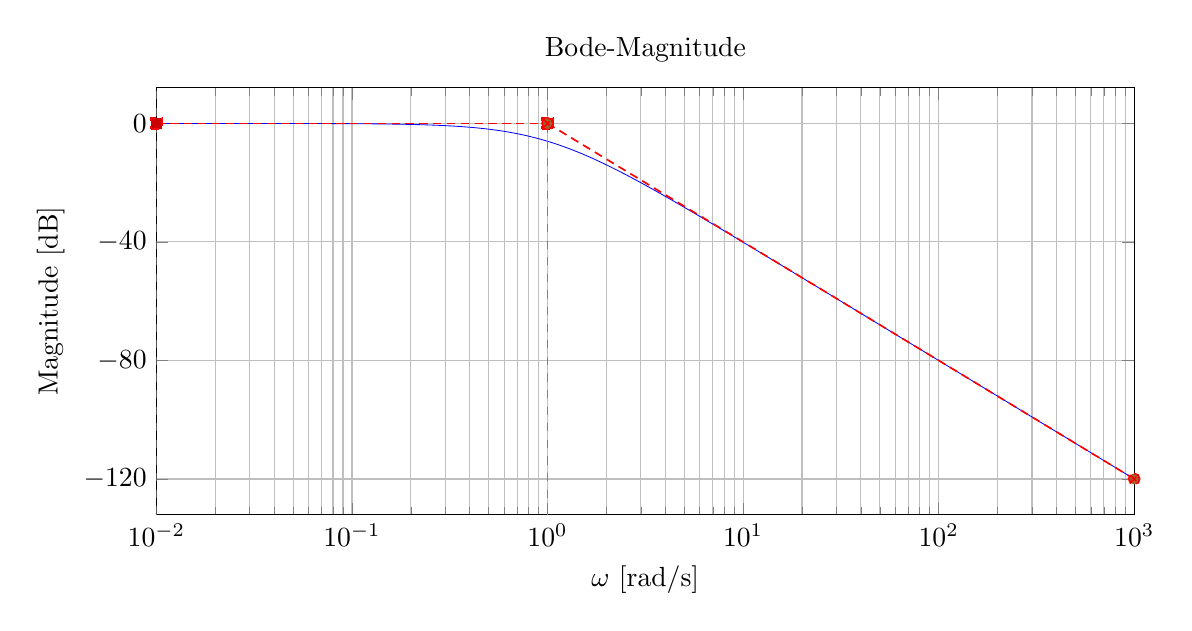
\begin{tikzpicture}
\begin{semilogxaxis}[
  width=14cm,height=7cm,
  xmin=1e-2,xmax=1e3,
  xlabel={$\omega$ [rad/s]},
  ylabel={Magnitude [dB]},
  grid=both,
  ytick distance=40,
  title={Bode-Magnitude}
]
\addplot[
  domain=1e-2:1e3,
  samples=600,
  mark=none,
  line width=0.3pt,
  blue
] {-40*ln(sqrt(1 + x^2))/ln(10)};
\addplot+[domain=1e-2:1,samples=2,dashed,dash pattern=on 3pt off 2pt,line width=0.6pt,red] {0};
\addplot+[domain=1:1e3,samples=2,dashed,dash pattern=on 3pt off 2pt,line width=0.6pt,red] {-40*ln(x)/ln(10)};
\draw[gray,dashed] (rel axis cs:0,0) -- (rel axis cs:0,1);
\draw[gray,dashed] (axis cs:1,\pgfkeysvalueof{/pgfplots/ymin}) -- (axis cs:1,\pgfkeysvalueof{/pgfplots/ymax});
\node[gray,anchor=south east] at (axis cs:1,\pgfkeysvalueof{/pgfplots/ymax}) {\scriptsize Pol $\omega_p=1$ (doppelt)};
\end{semilogxaxis}
\end{tikzpicture}
\vspace{6mm}
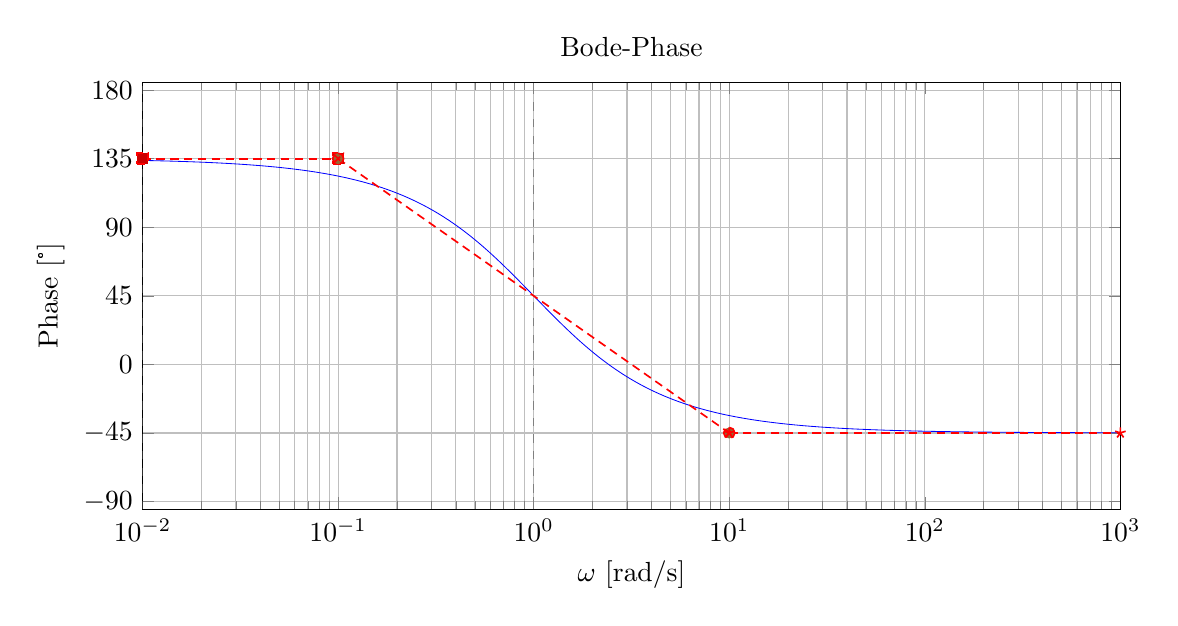
\begin{tikzpicture}
\begin{semilogxaxis}[
  width=14cm,height=7cm,
  xmin=1e-2,xmax=1e3,
  ymin=-95,ymax=185,
  ytick distance=45,
  xlabel={$\omega$ [rad/s]},
  ylabel={Phase [°]},
  grid=both,
  title={Bode-Phase}
]
\addplot[
  domain=1e-2:1e3,
  samples=600,
  mark=none,
  line width=0.3pt,
  blue
] {135 - 2*atan(x)};
\addplot+[domain=1e-2:1e-1,samples=2,dashed,dash pattern=on 3pt off 2pt,line width=0.6pt,red] {135};
\addplot+[domain=1e-1:1e1,samples=2,dashed,dash pattern=on 3pt off 2pt,line width=0.6pt,red] {45 - 90*ln(x)/ln(10)};
\addplot+[domain=1e1:1e3,samples=2,dashed,dash pattern=on 3pt off 2pt,line width=0.6pt,red] {-45};
\draw[gray,dashed] (rel axis cs:0,0) -- (rel axis cs:0,1);
\draw[gray,dashed] (axis cs:1,\pgfkeysvalueof{/pgfplots/ymin}) -- (axis cs:1,\pgfkeysvalueof{/pgfplots/ymax});
\node[gray,anchor=south east] at (axis cs:1,\pgfkeysvalueof{/pgfplots/ymax}) {\scriptsize Pol $\omega_p=1$ (doppelt)};
\end{semilogxaxis}
\end{tikzpicture}
\end{center}
\newpage

\subsection{Erklärung}
\begin{description}[leftmargin=1.2em,labelsep=.6em,font=\bfseries]

\item[1. Normalform herstellen.]
Bringe die Übertragungsfunktion in die Standardform.
\[
H(s)=\frac{K_0}{(1+sT_p)^2},\qquad
K_0=\frac{-1+\j}{\sqrt{2}}=\mathrm e^{\j 135^\circ},\quad T_p=1,\quad r=0.
\]
Zerlegung: \(\underline{F}_1(s)=\frac{1}{(1+sT_p)^2}\) (reelles Polglied zweiter Ordnung, doppelt); konstanter Phasor \(K_0\) mit \(|K_0|=1\), \(\arg K_0=+135^\circ\). Wir können $K_0$ behandeln als wäre es 1, aber müssen den gesamten Phasenplot um $135^\circ$ verschieben.

\item[2. Eckfrequenz bestimmen und sortieren.]
\[
\omega_p=\frac{1}{T_p}=1\,\mathrm{rad/s}.
\]
Nur diese Eckfrequenz; Sortierung trivial.

\item[3. Startpunkt des Amplitudengangs festlegen (Geradennäherung).]
\[
\omega_{\min}=\omega_p=1,\quad
F_{\mathrm{dB}}(\omega_{\min})=20\log_{10}\!\big(|K_0\underline{F}_{ges}^*(0)|\cdot \omega_{\min}^{\,r}\big)=0\,\mathrm{dB}.
\]
Anker für die Geradennäherung: \(0\,\mathrm{dB}\) bei \(\omega=1\).

\item[4. Verlauf links vom Startpunkt zeichnen.]
Für \(\omega<\omega_{min}\) bleibt die Amplituden-Asymptote bei \(0\,\mathrm{dB}\) konstant (Anfangssteigung \(r\cdot 20 \,\mathrm{dB}=0\)). Zeichne eine waagrechte Gerade links von der kleinsten Eckfrequenz.


\item[5. Steigungswechsel an der Eckfrequenz eintragen.]
Doppelpol: ab \(\omega=1\) Steigungsänderung um \(-40\,\mathrm{dB/dec}\).
Geradennäherung rechts:
\[
|H(j\omega)|_{\mathrm{dB}}\approx -40\log_{10}\omega\quad(\omega\ge 1).
\]

\item[6. Eckabrundung korrekt berücksichtigen.]
Bei \(\omega=\omega_p\) weicht der exakte Betrag um \(-6\,\mathrm{dB}\) von der Asymptote ab (Summe zweier \(-3\,\mathrm{dB}\), da Doppelpol):
\[
|H(j1)|_{\mathrm{dB}}=-20\log_{10}(1+1)=-20\log_{10}2\approx -6\,\mathrm{dB}.
\]

\item[7. Phasenstartwert festlegen.]
Konstanter Phasor \(K_0\) liefert einen Offset \(+135^\circ\).
Für \(\omega\to 0\): \(\varphi(0)=+135^\circ\).

\item[8. Phasenänderung durch das Polglied eintragen.]
Ein Doppelpol bewirkt insgesamt \(-180^\circ\) über die Dekade \([0.1,10]\) (je \(-90^\circ\) pro einfachem Pol). Näherung:
\[
\varphi(\omega)\approx
\begin{cases}
+135^\circ,& \omega\le 0.1,\\
45^\circ-90^\circ\log_{10}\omega,& 0.1<\omega<10,\\
-45^\circ,& \omega\ge 10.
\end{cases}
\]

\item[9. Grenzwerte und Konsistenz prüfen.]
DC: \(|H(0)|=|K_0|=1\Rightarrow 0\,\mathrm{dB}\), \(\varphi(0)=+135^\circ\).
HF: \(|H(j\omega)|\sim 1/\omega^{2}\Rightarrow -40\log_{10}\omega\,\mathrm{dB}\), \(\varphi(\infty)=+135^\circ-180^\circ=-45^\circ\).
Pol-/Nullzählung: \(m=0\), \(n=2\Rightarrow (m-n)\cdot 90^\circ=-180^\circ\) plus Offset \(+135^\circ\) durch \(K_0\) ergibt \(-45^\circ\).

\end{description}

\subsubsection*{Stückweise Näherungen (für die Skizze)}
\[
|H(j\omega)|_{\mathrm{dB}}\approx
\begin{cases}
0,& \omega\ll 1,\\[2pt]
-20\log_{10}2,& \omega=1,\\[2pt]
-40\log_{10}\omega,& \omega\gg 1,
\end{cases}
\]\[
\varphi(\omega)\approx
\begin{cases}
+135^\circ,& \omega\le 0.1,\\[2pt]
45^\circ-90^\circ\log_{10}\omega,& 0.1<\omega<10,\\[2pt]
-45^\circ,& \omega\ge 10.
\end{cases}
\]

\newpage
\section{}
\[
H(s)=\frac{-1000}{(s+1)(s+100)}\,.
\]
\subsection{Bode-Diagramm}
\begin{center}
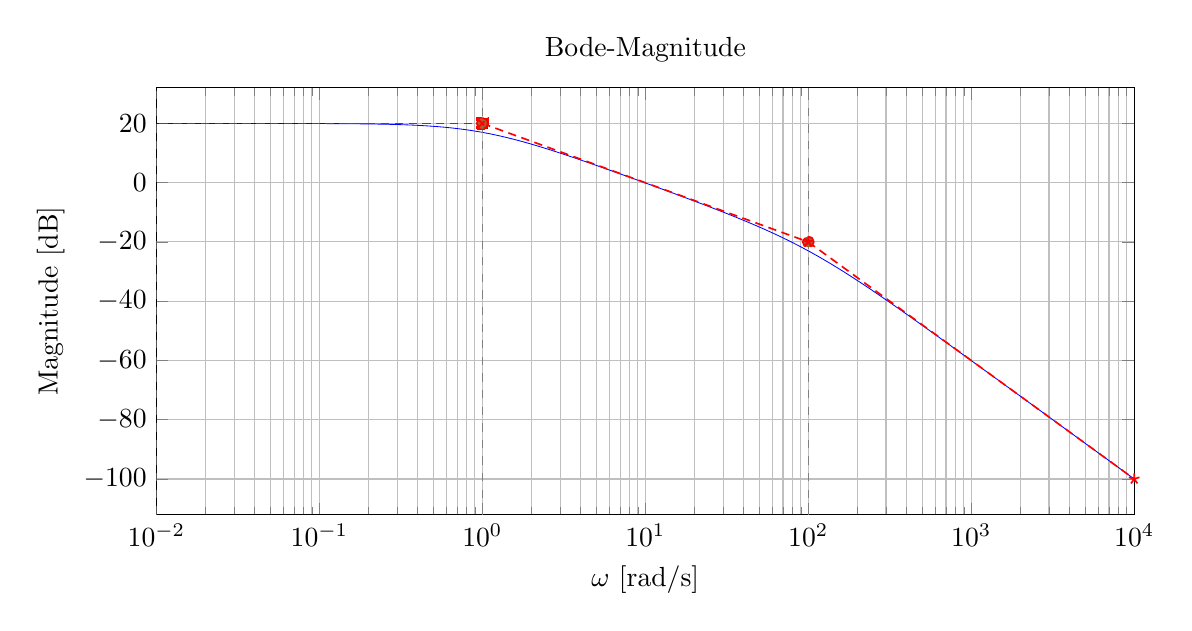
\begin{tikzpicture}
\begin{semilogxaxis}[
  width=14cm,height=7cm,
  xmin=1e-2,xmax=1e4,
  ytick distance=20,
  xlabel={$\omega$ [rad/s]},
  ylabel={Magnitude [dB]},
  grid=both,
  title={Bode-Magnitude}
]
\addplot[
  domain=1e-3:1e4,
  samples=800,
  mark=none,
  line width=0.3pt,
  blue
] {60 - 20*ln(sqrt(1 + x^2))/ln(10) - 20*ln(sqrt(10000 + x^2))/ln(10)};
\addplot+[domain=1e-3:1,samples=2,dashed,dash pattern=on 3pt off 2pt,line width=0.6pt,red] {20};
\addplot+[domain=1:1e2,samples=2,dashed,dash pattern=on 3pt off 2pt,line width=0.6pt,red] {20 - 20*ln(x)/ln(10)};
\addplot+[domain=1e2:1e4,samples=2,dashed,dash pattern=on 3pt off 2pt,line width=0.6pt,red] {-20 - 40*ln(x/100)/ln(10)};
\draw[gray,dashed] (rel axis cs:0,0) -- (rel axis cs:0,1);
\draw[gray,dashed] (axis cs:1,\pgfkeysvalueof{/pgfplots/ymin}) -- (axis cs:1,\pgfkeysvalueof{/pgfplots/ymax});
\draw[gray,dashed] (axis cs:100,\pgfkeysvalueof{/pgfplots/ymin}) -- (axis cs:100,\pgfkeysvalueof{/pgfplots/ymax});
\node[gray,anchor=south east] at (axis cs:1,\pgfkeysvalueof{/pgfplots/ymax}) {\scriptsize Pol $\omega_p=1$};
\node[gray,anchor=south east] at (axis cs:100,\pgfkeysvalueof{/pgfplots/ymax}) {\scriptsize Pol $\omega_p=100$};
\end{semilogxaxis}
\end{tikzpicture}
\vspace{6mm}
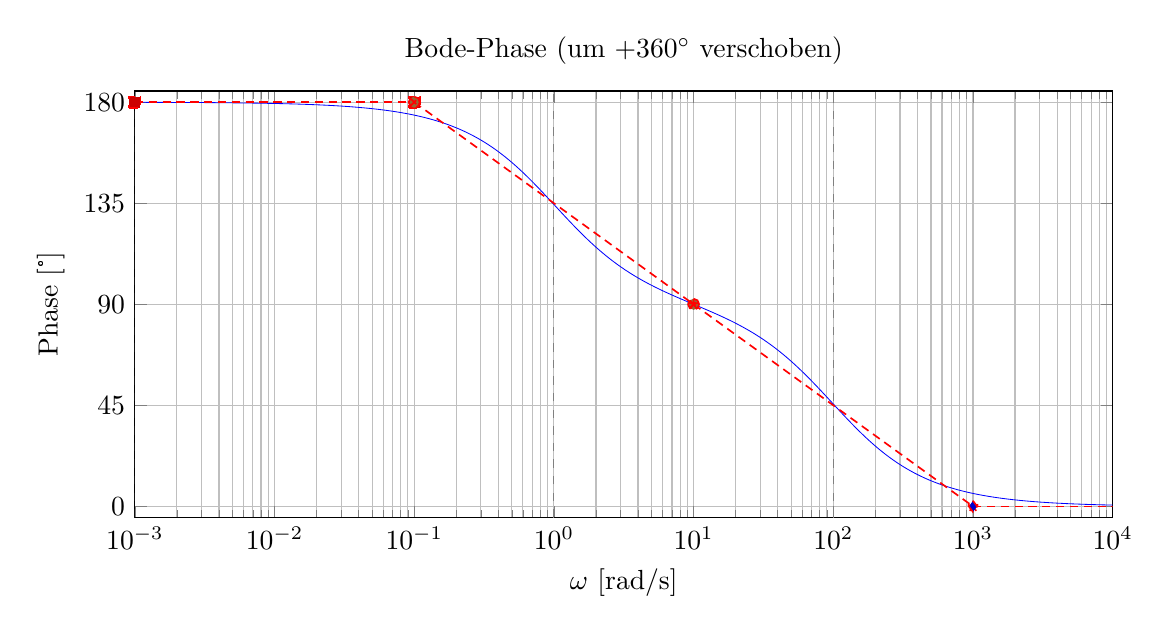
\begin{tikzpicture}
\begin{semilogxaxis}[
  width=14cm,height=7cm,
  xmin=1e-3,xmax=1e4,
  ymin=-5,ymax=185,
  ytick distance=45,
  xlabel={$\omega$ [rad/s]},
  ylabel={Phase [°]},
  grid=both,
  title={Bode-Phase (um $+360^\circ$ verschoben)}
]
\addplot[
  domain=1e-3:1e5,
  samples=800,
  mark=none,
  line width=0.3pt,
  blue
] {180 - atan(x) - atan(x/100)};
\addplot+[domain=1e-3:1e-1,samples=2,dashed,dash pattern=on 3pt off 2pt,line width=0.6pt,red] {180};
\addplot+[domain=1e-1:1e1,samples=2,dashed,dash pattern=on 3pt off 2pt,line width=0.6pt,red] {135 - 45*ln(x)/ln(10)};

\addplot+[domain=1e1:1e3,samples=2,dashed,dash pattern=on 3pt off 2pt,line width=0.6pt,red]{45 - 45*ln(x/100)/ln(10)};
\addplot+[domain=1e3:1e5,samples=2,dashed,dash pattern=on 3pt off 2pt,line width=0.6pt,red]{0};
\draw[gray,dashed] (rel axis cs:0,0) -- (rel axis cs:0,1);
\draw[gray,dashed] (axis cs:1,\pgfkeysvalueof{/pgfplots/ymin}) -- (axis cs:1,\pgfkeysvalueof{/pgfplots/ymax});
\draw[gray,dashed] (axis cs:100,\pgfkeysvalueof{/pgfplots/ymin}) -- (axis cs:100,\pgfkeysvalueof{/pgfplots/ymax});
\node[gray,anchor=south east] at (axis cs:1,\pgfkeysvalueof{/pgfplots/ymax}) {\scriptsize Pol $\omega_p=1$};
\node[gray,anchor=south east] at (axis cs:100,\pgfkeysvalueof{/pgfplots/ymax}) {\scriptsize Pol $\omega_p=100$};
\end{semilogxaxis}
\end{tikzpicture}
\end{center}
\newpage

\subsection{Erklärung}
\begin{description}[leftmargin=1.2em,labelsep=.6em,font=\bfseries]

\item[1. Normalform herstellen.]
\[
H(s)=\frac{-1000}{(s+1)(s+100)}
= \frac{K_0}{(1+sT_{p1})(1+sT_{p2})}
\]
mit
\[
K_0=-10,\quad r=0,\quad T_{p1}=1,\quad T_{p2}=\tfrac{1}{100}.
\]
\[
\underline{F}_1(s)=\frac{1}{1+sT_{p1}}=\frac{1}{1+s},\qquad
\underline{F}_2(s)=\frac{1}{1+sT_{p2}}=\frac{1}{1+\tfrac{s}{100}}.
\]
Konstantes Vorzeichen \(K_0<0\): Phasenoffset \(\pm180^\circ\) (hier Darstellung um \(+360^\circ\) verschoben).

\item[2. Eckfrequenzen bestimmen und sortieren.]Die $\omega$-Eckfrequenzen lassen sich aus den $T_n$'s bestimmen und müssen anschließend sortiert werden:
\[
\omega_{p1}=\frac{1}{T_{p1}}=1\,\mathrm{rad/s},\qquad \omega_{p2}=\frac{1}{T_{p2}}=100\,\mathrm{rad/s},\qquad \omega_{p1}<\omega_{p2}.
\]

\item[3. Startpunkt des Amplitudengangs festlegen (Geradennäherung).]
\[
\omega_{\min}=\omega_{p1}=1,\quad
F_{\mathrm{dB}}(\omega_{\min})=20\log_{10}\!\big(|K_0\underline{F}_{ges}^*(0)|\,\omega_{\min}^{\,r}\big)=20\log_{10}10=20\,\mathrm{dB}.
\]
Unser Ankerpunkt ist: \(20\,\mathrm{dB}\) bei \(\omega=1\).

\item[4. Verlauf links vom Startpunkt zeichnen.]
Für \(\omega<\omega_z\) bleibt die Amplituden-Asymptote bei \(20\,\mathrm{dB}\) konstant (Anfangssteigung \(r\cdot 20 \,\mathrm{dB}=0\)). Zeichne eine waagrechte Gerade links von der kleinsten Eckfrequenz.

\item[5. Steigungswechsel an den Eckfrequenzen eintragen.]
Ab \(\omega=1\): \(-20\,\mathrm{dB/dec}\) (einfacher Pol).
Ab \(\omega=100\): zusätzl. \(-20\,\mathrm{dB/dec}\) \(\Rightarrow\) insgesamt \(-40\,\mathrm{dB/dec}\).
Geradennäherungen:
\[
|H(j\omega)|_{\mathrm{dB}}\approx
\begin{cases}
20,& \omega\le 1,\\
20-20\log_{10}\omega,& 1<\omega\le 100,\\
-20-40\log_{10}(\omega/100),& \omega\ge 100.
\end{cases}
\]

\item[6. Eckabrundungen korrekt berücksichtigen.]
Bei jedem einfachen Pol: \(-3\,\mathrm{dB}\) am Knick.
\[
|H(j1)|_{\mathrm{dB}}=20-10\log_{10}2\approx 17\,\mathrm{dB},\qquad
|H(j100)|_{\mathrm{dB}}=-20-10\log_{10}2\approx -23\,\mathrm{dB}.
\]

\item[7. Phasenstartwert festlegen.]
Wegen \(K_0<0\): Startphase \(-180^\circ + r\cdot90^\circ=-180^\circ\). Darstellung um \(+360^\circ\) verschoben \(\Rightarrow\) \(+180^\circ\) für \(\omega\ll 0.1\).

\item[8. Phasenänderung durch die Polglieder eintragen.]
Jeder einfache Pol: \(-90^\circ\) über je eine Dekade.
Näherung (verschobene Darstellung):
\[
\varphi(\omega)\approx
\begin{cases}
180^\circ,& \omega\le 0.1,\\
135^\circ-45^\circ\log_{10}\omega,& 0.1<\omega<10,\\
45^\circ-45^\circ\log_{10}(\omega/100),& 10<\omega<1000,\\
0^\circ,& \omega\ge 1000.
\end{cases}
\]

\item[9. Grenzwerte und Konsistenz prüfen.]
DC: \(|H(0)|=10\Rightarrow 20\,\mathrm{dB}\); Phase \(-180^\circ\) (hier als \(+180^\circ\) gezeigt).
HF: \(|H(j\omega)|\sim 10/\omega^2\Rightarrow -40\log_{10}(\omega/100)-20\,\mathrm{dB}\). 
Pol-/Nullzählung bestätigt die Endphase: \(m=0\), \(n=2\Rightarrow (m-n)\cdot 90^\circ=-180^\circ\); plus negatives \(K_0\) \(\Rightarrow\) zusätzlich \(-180^\circ\); gesamte \(-360^\circ\equiv 0^\circ\) (mod \(360^\circ\)).

\end{description}

\subsubsection*{Stückweise Näherungen (für die Skizze)}
\[
|H(j\omega)|_{\mathrm{dB}}\approx
\begin{cases}
20,& \omega\ll 1,\\[2pt]
20-10\log_{10}2,& \omega=1,\\[2pt]
20-20\log_{10}\omega,& 1\ll\omega\ll 100,\\[2pt]
-20-10\log_{10}2,& \omega=100,\\[2pt]
-20-40\log_{10}(\omega/100),& \omega\gg 100,
\end{cases}
\]\[
\varphi(\omega)\ (\text{um }+360^\circ)\approx
\begin{cases}
180^\circ,& \omega\le 0.1,\\[2pt]
135^\circ-45^\circ\log_{10}\omega,& 0.1<\omega<10,\\[2pt]
45^\circ-45^\circ\log_{10}(\omega/100),& 10<\omega<1000,\\[2pt]
0^\circ,& \omega\ge 1000.
\end{cases}
\]

\newpage
\section{}
\[
H(s)=\frac{100\,s}{s+1}\,.
\]
\subsection{Bode-Diagramm}
\begin{center}
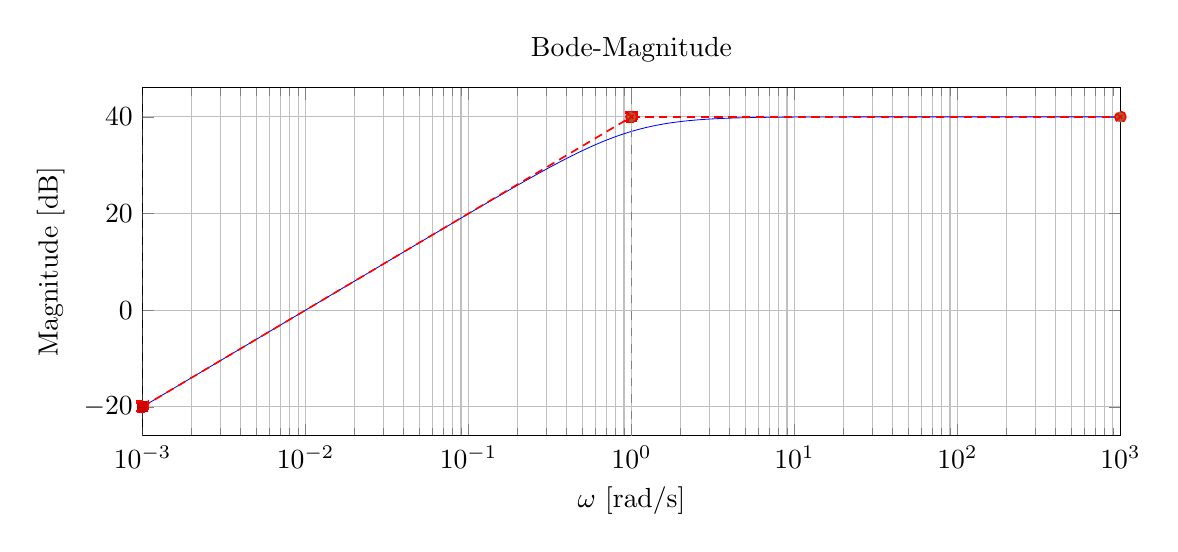
\begin{tikzpicture}
\begin{semilogxaxis}[
  width=14cm,height=6cm,
  xmin=1e-3,xmax=1e3,
  xlabel={$\omega$ [rad/s]},
  ylabel={Magnitude [dB]},
  grid=both,
  title={Bode-Magnitude}
]
\addplot[
  domain=1e-3:1e3,
  samples=600,
  mark=none,
  line width=0.3pt,
  blue
] {40 + 20*ln(x)/ln(10) - 20*ln(sqrt(1 + x^2))/ln(10)};
\addplot+[domain=1e-3:1,samples=2,dashed,dash pattern=on 3pt off 2pt,line width=0.6pt,red] {40 + 20*ln(x)/ln(10)};
\addplot+[domain=1:1e3,samples=2,dashed,dash pattern=on 3pt off 2pt,line width=0.6pt,red] {40};
\draw[gray,dashed] (rel axis cs:0,0) -- (rel axis cs:0,1);
\draw[gray,dashed] (axis cs:1,\pgfkeysvalueof{/pgfplots/ymin}) -- (axis cs:1,\pgfkeysvalueof{/pgfplots/ymax});
\node[gray,anchor=south east] at (axis cs:1,\pgfkeysvalueof{/pgfplots/ymax}) {\scriptsize Pol $\omega_p=1$};
\end{semilogxaxis}
\end{tikzpicture}
\vspace{6mm}
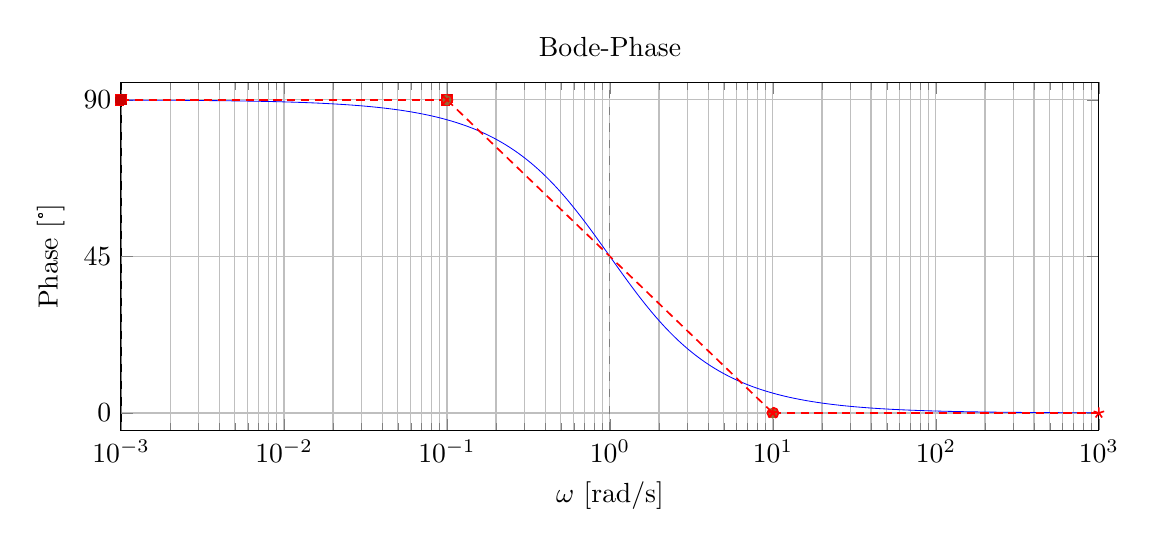
\begin{tikzpicture}
\begin{semilogxaxis}[
  width=14cm,height=6cm,
  xmin=1e-3,xmax=1e3,
  ymin=-5,ymax=95,
  xlabel={$\omega$ [rad/s]},
  ylabel={Phase [°]},
  grid=both,
  ytick distance=45,
  title={Bode-Phase}
]
\addplot[
  domain=1e-3:1e3,
  samples=600,
  mark=none,
  line width=0.3pt,
  blue
] {90 - atan(x)};
\addplot+[domain=1e-3:1e-1,samples=2,dashed,dash pattern=on 3pt off 2pt,line width=0.6pt,red] {90};
\addplot+[domain=1e-1:1e1,samples=2,dashed,dash pattern=on 3pt off 2pt,line width=0.6pt,red] {45 - 45*ln(x)/ln(10)};
\addplot+[domain=1e1:1e3,samples=2,dashed,dash pattern=on 3pt off 2pt,line width=0.6pt,red] {0};
\draw[gray,dashed] (rel axis cs:0,0) -- (rel axis cs:0,1);
\draw[gray,dashed] (axis cs:1,\pgfkeysvalueof{/pgfplots/ymin}) -- (axis cs:1,\pgfkeysvalueof{/pgfplots/ymax});
\node[gray,anchor=south east] at (axis cs:1,\pgfkeysvalueof{/pgfplots/ymax}) {\scriptsize Pol $\omega_p=1$};
\end{semilogxaxis}
\end{tikzpicture}
\end{center}
\newpage
\subsection{Erklärung (ausführlich)}
\begin{description}[leftmargin=1.2em,labelsep=.6em,font=\bfseries]

\item[1. Zuerst Normalform herstellen.]
\[
H(s)=\frac{100s}{s+1}=100\cdot s\cdot \frac{1}{\,(1+sT_p)}
\]
Die Teilglieder und Variablen gemäß Skript sind: 
\[
\underline{F}_1(s)=\frac{1}{1+s},\;T_p=1,\;K_0=100\;\text{und}\;r=0.
\]


\item[2. Danach Eckfrequenz bestimmen und sortieren.]
\[
\omega_p=\frac{1}{T_p}=1\,\mathrm{rad/s}.
\]
Diese ist die einzige Eckfrequenz, daher ist eine Sortierung der Eckfrequenzen hier hinfällig.

\item[3. Startpunkt des Amplitudengangs festlegen (Geradennäherung).]
Setze $\omega_{\min}=\omega_p=1$.
\[
F_{\mathrm{dB}}(\omega_{\min})=20\log_{10}\!\big(|K_0\,F^*_{ges}(0)|\,\omega_{\min}^{\,r}\big)
=20\log_{10}(100\cdot 1\cdot 1)=40\,\mathrm{dB}.
\]
Anfangssteigung $r\cdot 20\,\mathrm{dB/dec}=+20\,\mathrm{dB/dec}$.

\item[4. Verlauf links vom Startpunkt.]
Für $\omega<\omega_{\min}=1$ gilt die Geradennäherung mit Steigung $+20\,\mathrm{dB/dec}$. Einzeichnen als Gerade mit Steigung $+20\,\mathrm{dB/dec}$ durch den Punkt $(\omega_{\min},\,40\,\mathrm{dB})$.


\item[5. Steigungswechsel an der Eckfrequenz eintragen.]
$\underline{F}_2$ reduziert ab $\omega_p$ die Steigung um $20\,\mathrm{dB/dec}$:
\[
\omega<1:\ +20\,\mathrm{dB/dec},\qquad \omega\ge 1:\ 0\,\mathrm{dB/dec}.
\]

\item[6. Eckabrundung korrekt berücksichtigen.]
\[
|H(j\omega)|=\frac{100\,\omega}{\sqrt{1+\omega^2}},\qquad
|H(j\cdot 1)|_{\mathrm{dB}}=40-10\log_{10}2\approx 36.99\,\mathrm{dB}.
\]
Bei $\omega=1$ liegt die Kurve etwa $3.01\,\mathrm{dB}$ unter der rechten Asymptote.
\newpage
\item[7. Phasenstartwert festlegen.]
Da $K_0F_{\mathrm{ges}}(0)>0$ und $r=1$ gilt
\[
\varphi(0)=\arg\!\big(K_0F_{\mathrm{ges}}(0)\big)+r\cdot90^\circ
=0^\circ+1\cdot90^\circ=+90^\circ.
\]


\item[8. Phasenänderung durch die Teilglieder eintragen.]
für $\omega \ll 0.1$: konstante $+90^\circ$.
Wegen $\underline{F}_1$ (Pol 1. Ordnung) sinkt die Phase von $90^\circ\to 0^\circ$ über $[0.1,10]$ ab.
Geradennäherung gesamt:
\[
\varphi(\omega)\approx
\begin{cases}
+90^\circ,& \omega\le 0.1,\\
45^\circ-45^\circ\log_{10}\omega,& 0.1<\omega<10,\\
0^\circ,& \omega\ge 10.
\end{cases}
\]

\item[9. Grenzwerte und Konsistenz prüfen.]
DC: $|H(0)|=0\mathrel{\widehat{=}} -\infty\, \mathrm{dB},\ \varphi(0)=90^\circ$.
HF: $|H(j\omega)|\to 100\Rightarrow 40\,\mathrm{dB}$.

Pol-/Nullzählung: Zählergrad $m=1$, Nennergrad $n=1\Rightarrow \varphi(\infty)=(m-n)\cdot90^\circ=0^\circ$.
\end{description}

\subsubsection*{Stückweise Näherungen (für die Skizze)}
\[
|H(j\omega)|_{\mathrm{dB}}\approx
\begin{cases}
40+20\log_{10}\omega,& \omega\ll 1,\\[2pt]
40-10\log_{10}2,& \omega=1,\\[2pt]
40,& \omega\gg 1,
\end{cases}
\qquad
\varphi(\omega)\approx
\begin{cases}
+90^\circ,& \omega\le 0.1,\\[2pt]
45^\circ-45^\circ\log_{10}\omega,& 0.1<\omega<10,\\[2pt]
0^\circ,& \omega\ge 10.
\end{cases}
\]

\newpage
\section{}
\[
H(s)=\frac{10\sqrt{2}\,s^{2}}{s-1}\,.
\]
\subsection{Bode-Diagramm}
\begin{center}
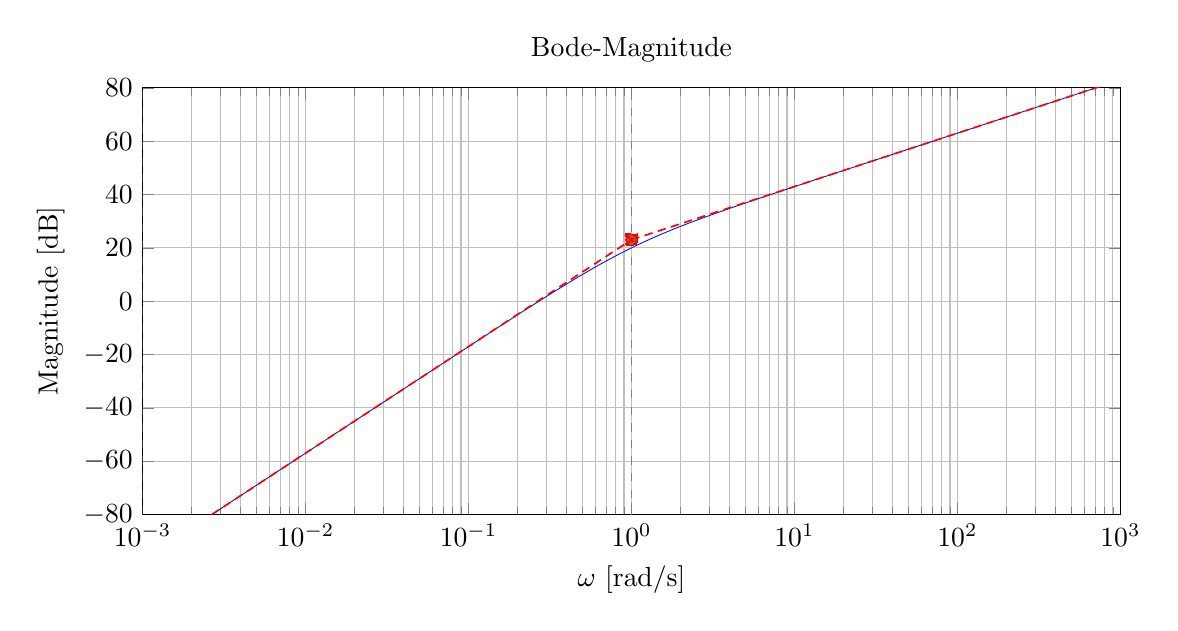
\begin{tikzpicture}
\begin{semilogxaxis}[
  width=14cm,height=7cm,
  xmin=1e-3,xmax=1e3,
  ymin=-80,ymax=80,
  xlabel={$\omega$ [rad/s]},
  ylabel={Magnitude [dB]},
  ytick distance=20,
  grid=both,
  title={Bode-Magnitude}
]
\addplot[
  domain=1e-3:1e3,
  samples=600,
  mark=none,
  line width=0.3pt,
  blue
] {20 + 10*ln(2)/ln(10) + 40*ln(x)/ln(10) - 10*ln(1 + x^2)/ln(10)};
\addplot+[domain=1e-3:1,samples=2,dashed,dash pattern=on 3pt off 2pt,line width=0.6pt,red] {20 + 10*ln(2)/ln(10) + 40*ln(x)/ln(10)};
\addplot+[domain=1:1e3,samples=2,dashed,dash pattern=on 3pt off 2pt,line width=0.6pt,red] {20 + 10*ln(2)/ln(10) + 20*ln(x)/ln(10)};
\draw[gray,dashed] (rel axis cs:0,0) -- (rel axis cs:0,1);
\draw[gray,dashed] (axis cs:1,\pgfkeysvalueof{/pgfplots/ymin}) -- (axis cs:1,\pgfkeysvalueof{/pgfplots/ymax});
\node[gray,anchor=south east] at (axis cs:1,\pgfkeysvalueof{/pgfplots/ymax}) {\scriptsize Pol $\omega_p=1$ (RHP)};
\end{semilogxaxis}
\end{tikzpicture}
\vspace{6mm}
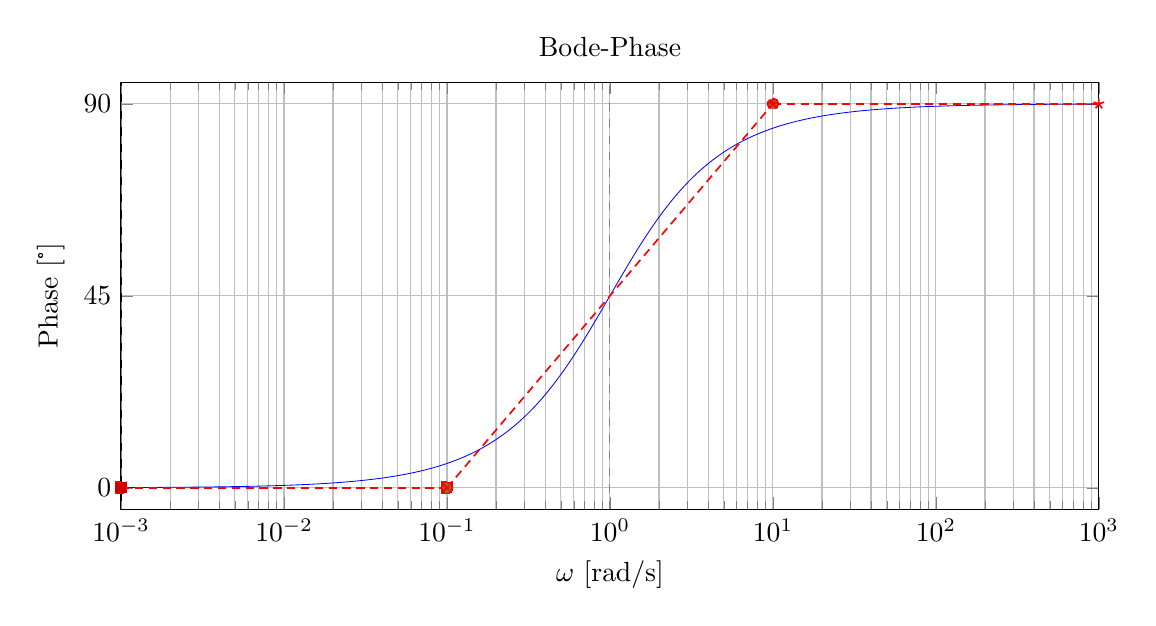
\begin{tikzpicture}
\begin{semilogxaxis}[
  width=14cm,height=7cm,
  xmin=1e-3,xmax=1e3,
  ymin=-5,ymax=95,
  ytick distance=45,
  xlabel={$\omega$ [rad/s]},
  ylabel={Phase [°]},
  grid=both,
  title={Bode-Phase}
]
\addplot[
  domain=1e-3:1e3,
  samples=600,
  mark=none,
  line width=0.3pt,
  blue
] {atan(x)};
\addplot+[domain=1e-3:1e-1,samples=2,dashed,dash pattern=on 3pt off 2pt,line width=0.6pt,red] {0};
\addplot+[domain=1e-1:1e1,samples=2,dashed,dash pattern=on 3pt off 2pt,line width=0.6pt,red] {45 + 45*ln(x)/ln(10)};
\addplot+[domain=1e1:1e3,samples=2,dashed,dash pattern=on 3pt off 2pt,line width=0.6pt,red] {90};
\draw[gray,dashed] (rel axis cs:0,0) -- (rel axis cs:0,1);
\draw[gray,dashed] (axis cs:1,\pgfkeysvalueof{/pgfplots/ymin}) -- (axis cs:1,\pgfkeysvalueof{/pgfplots/ymax});
\node[gray,anchor=south east] at (axis cs:1,\pgfkeysvalueof{/pgfplots/ymax}) {\scriptsize Pol $\omega_p=1$ (RHP)};
\end{semilogxaxis}
\end{tikzpicture}
\end{center}
\newpage
\subsection{Erklärung}
\vspace{5mm}
\begin{description}[leftmargin=1.2em,labelsep=.6em,font=\bfseries]
\item[Schritt 1] Doppelnullstelle im Ursprung: Startsteigung $+40\,\mathrm{dB/dec}$; Startphase $0^\circ$.
\item[Schritt 2] RHP-Pol bei $\omega_p=1\,\mathrm{rad/s}$: ab $\omega=1$ Steigungsänderung $-20\,\mathrm{dB/dec}$; Netto $+20\,\mathrm{dB/dec}$ für $\omega\gg1$. Phasen-Geradennäherung in $45^\circ$-Schritten: $0^\circ$ für $\omega\le0.1$, $45^\circ+45\log_{10}\omega$ in $[0.1,10]$, $90^\circ$ für $\omega\ge10$.
\item[Schritt 3] Grenzwerte: $|H|_{\mathrm{dB}}\approx 20+10\log_{10}2+40\log_{10}\omega$ für $\omega\ll1$, und $20+10\log_{10}2+20\log_{10}\omega$ für $\omega\gg1$; $\angle H\to90^\circ$ für große $\omega$.
\end{description}

\vspace{0.5cm}
\medskip
\noindent\textbf{Stückweise Näherung}
\[
|H(\j\omega)|_{\mathrm{dB}}\approx
\begin{cases}
20+10\log_{10}2+40\log_{10}\omega,& \omega\ll1,\\[4pt]
20,& \omega=1,\\[4pt]
20+10\log_{10}2+20\log_{10}\omega,& \omega\gg1,
\end{cases}
\qquad
\]
\newpage 
\section{}
\[
H(s)=\frac{s+1}{(s+10)^2}\,.
\]
\subsection{Bode-Diagramm}
\begin{center}
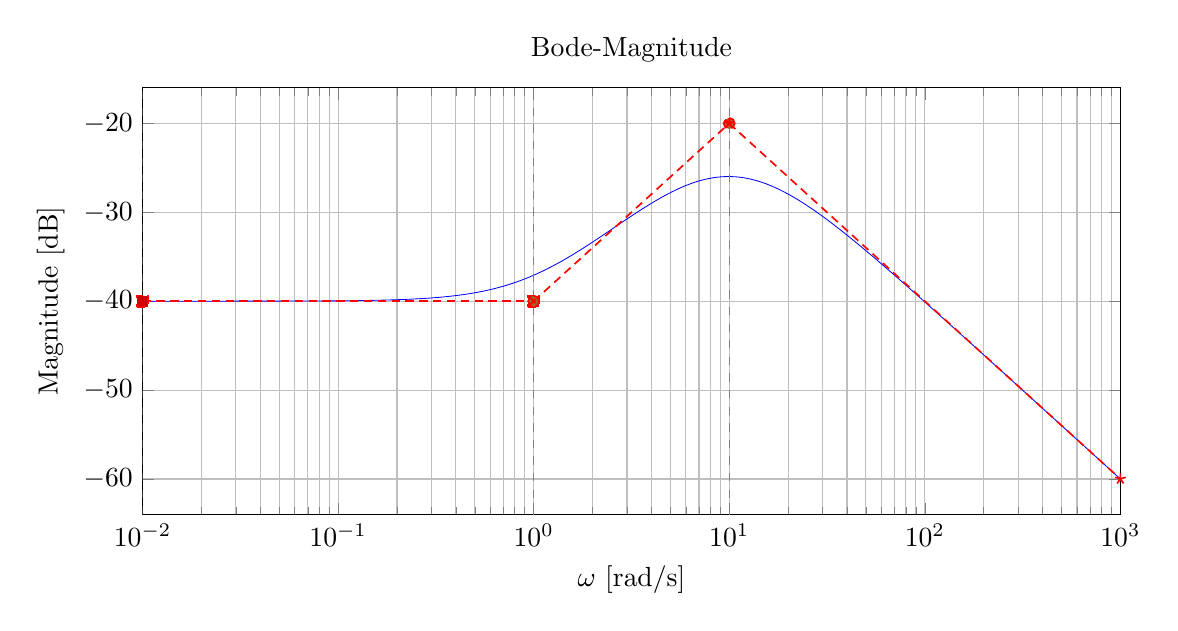
\begin{tikzpicture}
\begin{semilogxaxis}[
  width=14cm,height=7cm,
  xmin=1e-2,xmax=1e3,
  xlabel={$\omega$ [rad/s]},
  ylabel={Magnitude [dB]},
  grid=both,
  title={Bode-Magnitude}
]
\addplot[
  domain=1e-2:1e3,
  samples=600,
  mark=none,
  line width=0.3pt,
  blue
] {20*ln(sqrt(1 + x^2))/ln(10) - 40*ln(sqrt(100 + x^2))/ln(10)};
\addplot+[domain=1e-2:1,samples=2,dashed,dash pattern=on 3pt off 2pt,line width=0.6pt,red] {-40};
\addplot+[domain=1:1e1,samples=2,dashed,dash pattern=on 3pt off 2pt,line width=0.6pt,red] {-40 + 20*ln(x)/ln(10)};
\addplot+[domain=1e1:1e3,samples=2,dashed,dash pattern=on 3pt off 2pt,line width=0.6pt,red] {-20 - 20*ln(x/10)/ln(10)};
\draw[gray,dashed] (rel axis cs:0,0) -- (rel axis cs:0,1);
\draw[gray,dashed] (axis cs:1,\pgfkeysvalueof{/pgfplots/ymin}) -- (axis cs:1,\pgfkeysvalueof{/pgfplots/ymax});
\draw[gray,dashed] (axis cs:10,\pgfkeysvalueof{/pgfplots/ymin}) -- (axis cs:10,\pgfkeysvalueof{/pgfplots/ymax});
\node[gray,anchor=south east] at (axis cs:1,\pgfkeysvalueof{/pgfplots/ymax}) {\scriptsize Nullstelle $\omega_z=1$};
\node[gray,anchor=south east] at (axis cs:10,\pgfkeysvalueof{/pgfplots/ymax}) {\scriptsize Pol $\omega_p=10$ (doppelt)};
\end{semilogxaxis}
\end{tikzpicture}
\vspace{6mm}
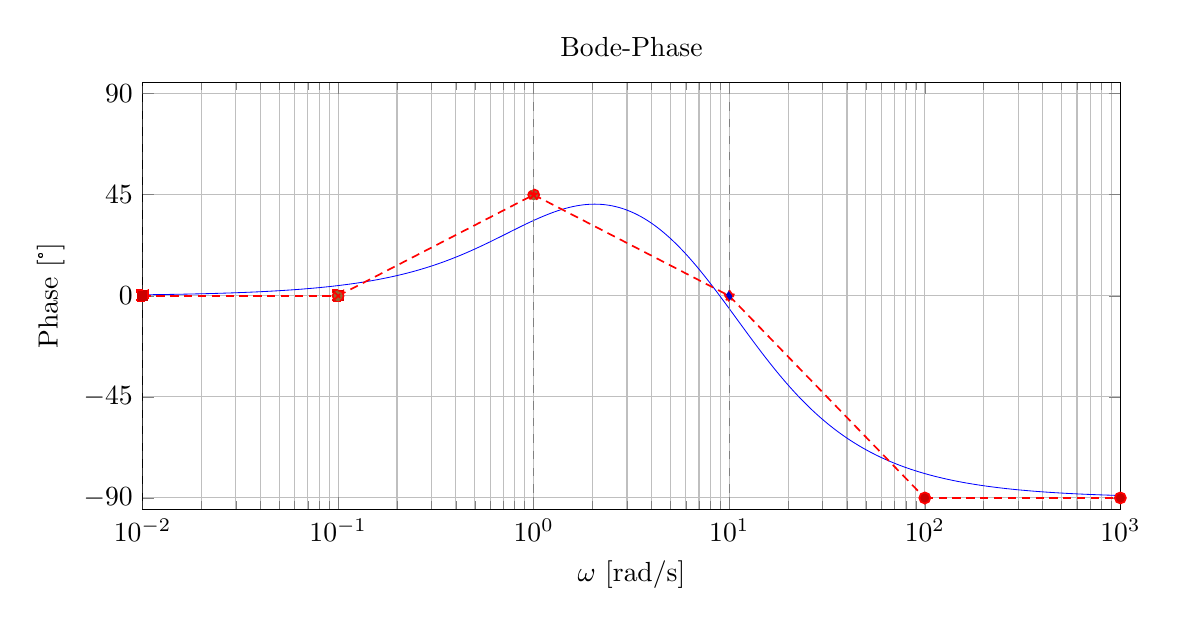
\begin{tikzpicture}
\begin{semilogxaxis}[
  width=14cm,height=7cm,
  xmin=1e-2,xmax=1e3,
  ytick distance=45,
  ymin=-95,ymax=95,
  xlabel={$\omega$ [rad/s]},
  ylabel={Phase [°]},
  grid=both,
  title={Bode-Phase}
]
\addplot[
  domain=1e-2:1e3,
  samples=600,
  mark=none,
  line width=0.3pt,
  blue
] {atan(x) - 2*atan(x/10)};
\addplot+[domain=1e-2:1e-1,samples=2,dashed,dash pattern=on 3pt off 2pt,line width=0.6pt,red] {0};
\addplot+[domain=1e-1:1e0,samples=2,dashed,dash pattern=on 3pt off 2pt,line width=0.6pt,red] {45 + 45*ln(x)/ln(10)};
\addplot+[domain=1e0:1e1,samples=2,dashed,dash pattern=on 3pt off 2pt,line width=0.6pt,red] {45 - 45*ln(x)/ln(10)};
\addplot+[domain=1e1:1e2,samples=2,dashed,dash pattern=on 3pt off 2pt,line width=0.6pt,red] {-90*ln(x/10)/ln(10)};
\addplot+[domain=1e2:1e3,samples=2,dashed,dash pattern=on 3pt off 2pt,line width=0.6pt,red] {-90};
\draw[gray,dashed] (rel axis cs:0,0) -- (rel axis cs:0,1);
\draw[gray,dashed] (axis cs:1,\pgfkeysvalueof{/pgfplots/ymin}) -- (axis cs:1,\pgfkeysvalueof{/pgfplots/ymax});
\draw[gray,dashed] (axis cs:10,\pgfkeysvalueof{/pgfplots/ymin}) -- (axis cs:10,\pgfkeysvalueof{/pgfplots/ymax});
\node[gray,anchor=south east] at (axis cs:1,\pgfkeysvalueof{/pgfplots/ymax}) {\scriptsize Nullstelle $\omega_z=1$};
\node[gray,anchor=south east] at (axis cs:10,\pgfkeysvalueof{/pgfplots/ymax}) {\scriptsize Pol $\omega_p=10$ (doppelt)};
\end{semilogxaxis}
\end{tikzpicture}
\end{center}
\newpage
\subsection{Erklärung}
\vspace{5mm}
\begin{description}[leftmargin=1.2em,labelsep=.6em,font=\bfseries]
\item[Schritt 1] DC-Faktor $\frac{1}{100}$: $H(s)=\dfrac{s+1}{(s+10)^2}$ liefert $H(0)=\tfrac{1}{100}$, daher Startniveau $-40\,\mathrm{dB}$ ohne Anfangssteigung; Startphase $\angle H(\j\omega)\approx0^\circ$ für $\omega\ll1$.
\item[Schritt 2] Nullstelle bei $\omega_z=1\,\mathrm{rad/s}$: ab $\omega=1$ steigt die Magnitude mit $+20\,\mathrm{dB/dec}$; bei $\omega=1$ liegt der exakte Betrag um $+10\log_{10}2\approx+3.01\,\mathrm{dB}$ über der Geradennäherung ($|H(\j1)|_{\mathrm{dB}}\approx-37.0\,\mathrm{dB}$). Phasenbeitrag der LHP-Nullstelle: Übergang $0^\circ\to+90^\circ$ über $\omega\in[0.1,10]$; Geradennäherung $+45^\circ+45^\circ\log_{10}\omega$ in $[0.1,1]$.
\item[Schritt 3] Doppelpol bei $\omega_p=10\,\mathrm{rad/s}$: ab $\omega=10$ zusätzliche Steigungsänderung um $-40\,\mathrm{dB/dec}$; Netto-Slope damit $-20\,\mathrm{dB/dec}$ für $\omega\gg10$ (asymptotisch $|H|\sim \omega/\omega^2=1/\omega$). Exakt bei $\omega=10$: $|H(\j10)|_{\mathrm{dB}}=-20-20\log_{10}2\approx-26.0\,\mathrm{dB}$ (d.\,h.\ $-6.02\,\mathrm{dB}$ unter der Geraden). Phasenbeitrag der beiden Pole: gemeinsamer Abfall um $180^\circ$ über $\omega\in[1,100]$; lineare Summe zweier Beiträge $(-45^\circ-45^\circ\log_{10}(\omega/10))$ ergibt die roten Segmente $45^\circ-45^\circ\log_{10}\omega$ für $\omega\in[1,10]$ und $-90^\circ\log_{10}(\omega/10)$ für $\omega\in[10,100]$. Grenzwerte: $\angle H\to0^\circ$ für $\omega\ll0.1$ und $\angle H\to-90^\circ$ für $\omega\gg100$.
\end{description}

\vspace{0.5cm}
\medskip
\noindent\textbf{Stückweise Näherung}
\[
|H(\j\omega)|_{\mathrm{dB}}\approx
\begin{cases}
-40,& \omega\ll1,\\[4pt]
-40+20\log_{10}\omega,& 1\ll\omega\ll10,\\[4pt]
-20-20\log_{10}(\omega/10),& \omega\gg10,
\end{cases}
\qquad
\]
\newpage
\section{}
\[
H(s)=\frac{s+1}{s^2+2s+1}=\frac{1}{s+1}\,.
\]
\subsection{Bode-Diagramm}
\begin{center}
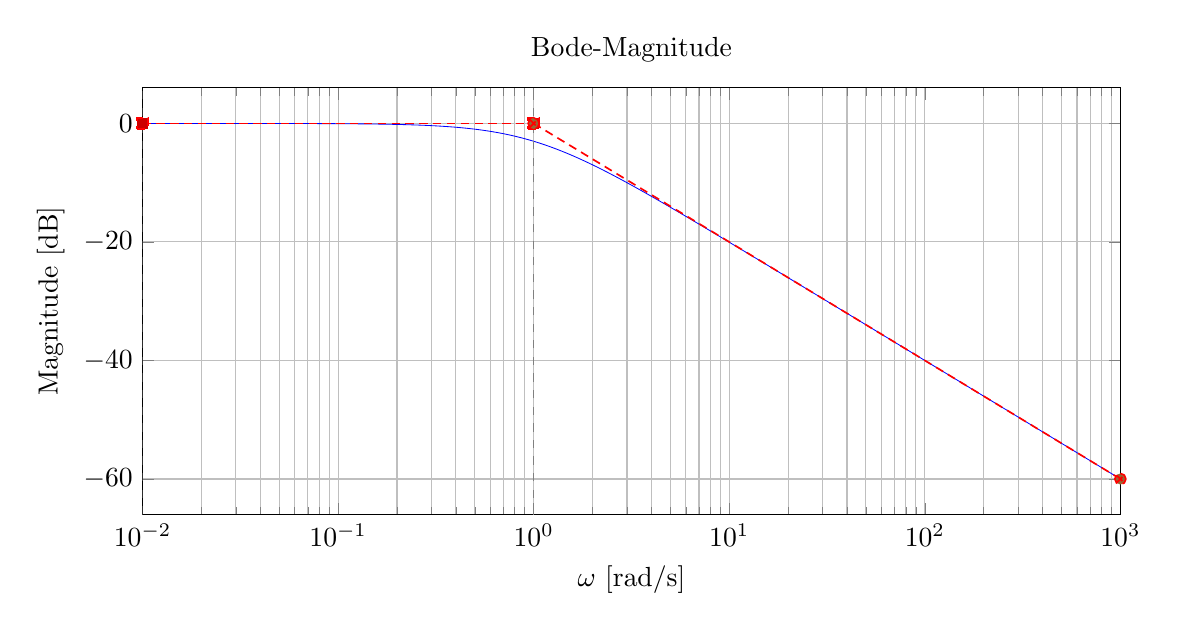
\begin{tikzpicture}
\begin{semilogxaxis}[
  width=14cm,height=7cm,
  xmin=1e-2,xmax=1e3,
  xlabel={$\omega$ [rad/s]},
  ylabel={Magnitude [dB]},
  grid=both,
  ytick distance=20,
  title={Bode-Magnitude}
]
\addplot[
  domain=1e-2:1e3,
  samples=600,
  mark=none,
  line width=0.3pt,
  blue
] {-20*ln(sqrt(1 + x^2))/ln(10)};
\addplot+[domain=1e-2:1,samples=2,dashed,dash pattern=on 3pt off 2pt,line width=0.6pt,red] {0};
\addplot+[domain=1:1e3,samples=2,dashed,dash pattern=on 3pt off 2pt,line width=0.6pt,red] {-20*ln(x)/ln(10)};
\draw[gray,dashed] (rel axis cs:0,0) -- (rel axis cs:0,1);
\draw[gray,dashed] (axis cs:1,\pgfkeysvalueof{/pgfplots/ymin}) -- (axis cs:1,\pgfkeysvalueof{/pgfplots/ymax});
\node[gray,anchor=south east] at (axis cs:1,\pgfkeysvalueof{/pgfplots/ymax}) {\scriptsize Pol $\omega_p=1$};
\end{semilogxaxis}
\end{tikzpicture}
\vspace{6mm}
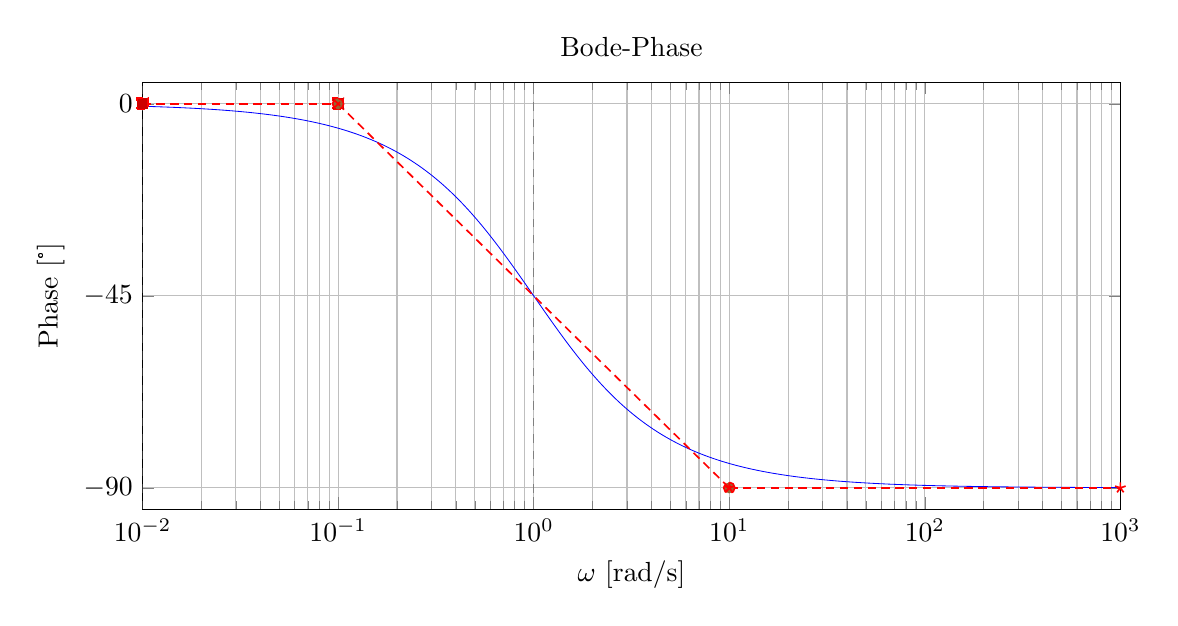
\begin{tikzpicture}
\begin{semilogxaxis}[
  width=14cm,height=7cm,
  xmin=1e-2,xmax=1e3,
  ymin=-95,ymax=5,
  ytick distance=45,
  xlabel={$\omega$ [rad/s]},
  ylabel={Phase [°]},
  grid=both,
  title={Bode-Phase}
]
\addplot[
  domain=1e-2:1e3,
  samples=600,
  mark=none,
  line width=0.3pt,
  blue
] {-atan(x)};
\addplot+[domain=1e-2:1e-1,samples=2,dashed,dash pattern=on 3pt off 2pt,line width=0.6pt,red] {0};
\addplot+[domain=1e-1:1e1,samples=2,dashed,dash pattern=on 3pt off 2pt,line width=0.6pt,red] {-45 - 45*ln(x)/ln(10)};
\addplot+[domain=1e1:1e3,samples=2,dashed,dash pattern=on 3pt off 2pt,line width=0.6pt,red] {-90};
\draw[gray,dashed] (rel axis cs:0,0) -- (rel axis cs:0,1);
\draw[gray,dashed] (axis cs:1,\pgfkeysvalueof{/pgfplots/ymin}) -- (axis cs:1,\pgfkeysvalueof{/pgfplots/ymax});
\node[gray,anchor=south east] at (axis cs:1,\pgfkeysvalueof{/pgfplots/ymax}) {\scriptsize Pol $\omega_p=1$};
\end{semilogxaxis}
\end{tikzpicture}
\end{center}
\newpage
\subsection{Erklärung}
\vspace{5mm}
\begin{description}[leftmargin=1.2em,labelsep=.6em,font=\bfseries]
\item[Schritt 1] Kürzung: $s^2+2s+1=(s+1)^2\Rightarrow H(s)=\dfrac{s+1}{(s+1)^2}=\dfrac{1}{s+1}$. DC-Faktor $1$: für $\omega\ll1$ gilt $|H(\j\omega)|\approx1$; Betrag $0\,\mathrm{dB}$ ohne Anfangssteigung, Phase $\approx0^\circ$.
\item[Schritt 2] Einfacher Pol bei $\omega_p=1\,\mathrm{rad/s}$: ab $\omega=1$ wechselt die Magnituden-Steigung um $-20\,\mathrm{dB/dec}$. Am Eckpunkt beträgt die exakte Dämpfung $-10\log_{10}2\approx-3\,\mathrm{dB}$ relativ zur Geraden. Phasenübergang über $\omega\in[0.1,10]$ von $0^\circ$ nach $-90^\circ$; Geradennäherung: $-45^\circ-45\log_{10}\omega$.
\item[Schritt 3] Grenzverhalten: für $\omega\gg1$ folgt $|H(\j\omega)|_{\mathrm{dB}}\approx-20\log_{10}\omega$; die Phase nähert sich $-90^\circ$. Für $\omega\ll1$ bleibt $|H|\approx1$ und $\angle H\approx0^\circ$.
\end{description}

\vspace{0.5cm}
\medskip
\noindent\textbf{Stückweise Näherung}
\[
|H(\j\omega)|_{\mathrm{dB}}\approx
\begin{cases}
0,& \omega\ll1,\\[4pt]
-10\log_{10}2,& \omega=1,\\[4pt]
-20\log_{10}\omega,& \omega\gg1,
\end{cases}
\qquad
\]
\newpage
\section{}
\[
H(s)=\frac{100\,(s+1)}{s^2+20s+100}=\frac{100\,(s+1)}{(s+10)^2}\,.
\]
\subsection{Bode-Diagramm}
\begin{center}
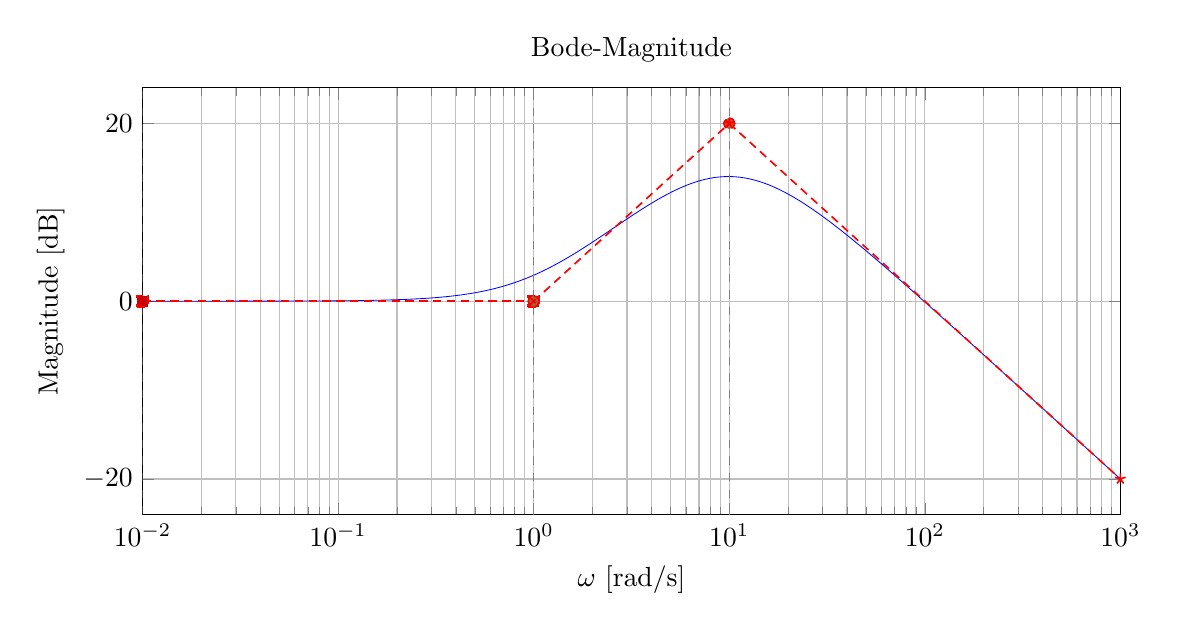
\begin{tikzpicture}
\begin{semilogxaxis}[
  width=14cm,height=7cm,
  xmin=1e-2,xmax=1e3,
  xlabel={$\omega$ [rad/s]},
  ylabel={Magnitude [dB]},
  grid=both,
  ytick distance=20,
  title={Bode-Magnitude}
]
\addplot[
  domain=1e-2:1e3,
  samples=600,
  mark=none,
  line width=0.3pt,
  blue
] {40 + 20*ln(sqrt(1 + x^2))/ln(10) - 40*ln(sqrt(100 + x^2))/ln(10)};
\addplot+[domain=1e-2:1,samples=2,dashed,dash pattern=on 3pt off 2pt,line width=0.6pt,red] {0};
\addplot+[domain=1:1e1,samples=2,dashed,dash pattern=on 3pt off 2pt,line width=0.6pt,red] {20*ln(x)/ln(10)};
\addplot+[domain=1e1:1e3,samples=2,dashed,dash pattern=on 3pt off 2pt,line width=0.6pt,red] {20 - 20*ln(x/10)/ln(10)};
\draw[gray,dashed] (rel axis cs:0,0) -- (rel axis cs:0,1);
\draw[gray,dashed] (axis cs:1,\pgfkeysvalueof{/pgfplots/ymin}) -- (axis cs:1,\pgfkeysvalueof{/pgfplots/ymax});
\draw[gray,dashed] (axis cs:10,\pgfkeysvalueof{/pgfplots/ymin}) -- (axis cs:10,\pgfkeysvalueof{/pgfplots/ymax});
\node[gray,anchor=south east] at (axis cs:1,\pgfkeysvalueof{/pgfplots/ymax}) {\scriptsize Nullstelle $\omega_z=1$};
\node[gray,anchor=south east] at (axis cs:10,\pgfkeysvalueof{/pgfplots/ymax}) {\scriptsize Pol $\omega_p=10$ (doppelt)};
\end{semilogxaxis}
\end{tikzpicture}
\vspace{6mm}
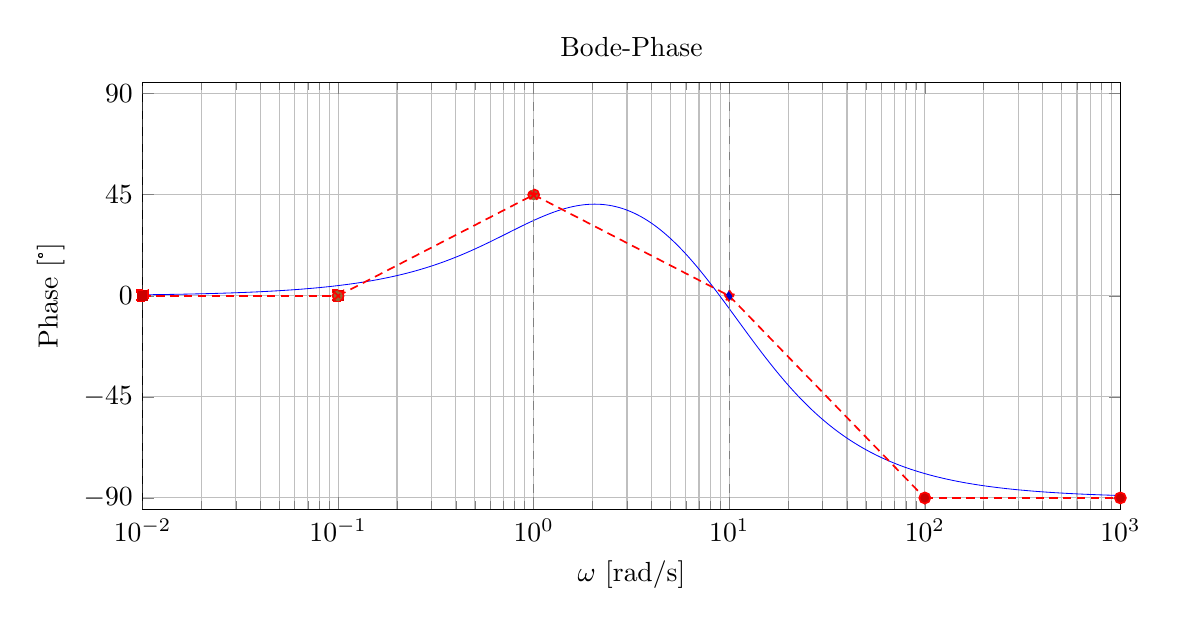
\begin{tikzpicture}
\begin{semilogxaxis}[
  width=14cm,height=7cm,
  xmin=1e-2,xmax=1e3,
  ymin=-95,ymax=95,
  ytick distance=45,
  xlabel={$\omega$ [rad/s]},
  ylabel={Phase [°]},
  grid=both,
  title={Bode-Phase}
]
\addplot[
  domain=1e-2:1e3,
  samples=600,
  mark=none,
  line width=0.3pt,
  blue
] {atan(x) - 2*atan(x/10)};
\addplot+[domain=1e-2:1e-1,samples=2,dashed,dash pattern=on 3pt off 2pt,line width=0.6pt,red] {0};
\addplot+[domain=1e-1:1e0,samples=2,dashed,dash pattern=on 3pt off 2pt,line width=0.6pt,red] {45 + 45*ln(x)/ln(10)};
\addplot+[domain=1e0:1e1,samples=2,dashed,dash pattern=on 3pt off 2pt,line width=0.6pt,red] {45 - 45*ln(x)/ln(10)};
\addplot+[domain=1e1:1e2,samples=2,dashed,dash pattern=on 3pt off 2pt,line width=0.6pt,red] {-90*ln(x/10)/ln(10)};
\addplot+[domain=1e2:1e3,samples=2,dashed,dash pattern=on 3pt off 2pt,line width=0.6pt,red] {-90};
\draw[gray,dashed] (rel axis cs:0,0) -- (rel axis cs:0,1);
\draw[gray,dashed] (axis cs:1,\pgfkeysvalueof{/pgfplots/ymin}) -- (axis cs:1,\pgfkeysvalueof{/pgfplots/ymax});
\draw[gray,dashed] (axis cs:10,\pgfkeysvalueof{/pgfplots/ymin}) -- (axis cs:10,\pgfkeysvalueof{/pgfplots/ymax});
\node[gray,anchor=south east] at (axis cs:1,\pgfkeysvalueof{/pgfplots/ymax}) {\scriptsize Nullstelle $\omega_z=1$};
\node[gray,anchor=south east] at (axis cs:10,\pgfkeysvalueof{/pgfplots/ymax}) {\scriptsize Pol $\omega_p=10$ (doppelt)};
\end{semilogxaxis}
\end{tikzpicture}
\end{center}
\newpage
\subsection{Erklärung}
\begin{description}[leftmargin=1.2em,labelsep=.6em,font=\bfseries]

\item[1. Normalform herstellen.]
\[
H(s)=\frac{100(s+1)}{(s+10)^2}
= K_0\cdot(1+sT_z)\cdot\frac{1}{(1+sT_p)^2}
\]
mit
\[
K_0=1,\quad r=0,\quad T_z=1,\quad T_p=\tfrac{1}{10}.
\]
\[
\underline{F}_1(s)=1+sT_z\quad\text{(LHP-Nullstelle)},\qquad
\underline{F}_2(s)=\frac{1}{(1+sT_p)^2}\quad\text{(Doppelpol)}.
\]

\item[2. Eckfrequenzen bestimmen und sortieren.] Die $\omega$-Eckfrequenzen aus den $T_n$ bestimmen und sortieren:
\[
\omega_z=\frac{1}{T_z}=1\,\mathrm{rad/s},\qquad
\omega_p=\frac{1}{T_p}=10\,\mathrm{rad/s},\qquad
\omega_z<\omega_p.
\]

\item[3. Startpunkt des Amplitudengangs festlegen (Geradennäherung).]
Setze \(\omega_{\min}=\omega_z=1\).
\[
F_{\mathrm{dB}}(\omega_{\min})=20\log_{10}\!\Big(|K_0F^*_{ges}(0)|\,\omega_{\min}^{\,r}\Big)
=20\log_{10}(1)=0\,\mathrm{dB}.
\]
Ankerpunkt: \(0\,\mathrm{dB}\) bei \(\omega=1\).

\item[4. Verlauf links vom Startpunkt zeichnen.]
Für \(\omega<1\) bleibt die Amplituden-Asymptote bei \(0\,\mathrm{dB}\) konstant (Anfangssteigung \(r\cdot 20\,\mathrm{dB/dec}=0\)). Zeichne links von der kleinsten Eckfrequenz eine waagrechte Gerade bei \(0\,\mathrm{dB}\).

\item[5. Steigungswechsel an den Eckfrequenzen eintragen.]
Nullstelle bei \(\omega_z=1\) bewirkt eine Steigungsänderung um \(+20\,\mathrm{dB/dec}\) ab \(\omega=1\).
Doppelpol bei \(\omega_p=10\) ändert die Magnitudensteigung um zusätzlich \(-40\,\mathrm{dB/dec}\) ab \(\omega=10\).
Netto:
\[
\begin{cases}
0\,\mathrm{dB}\ \text{(flach)},& \omega<1,\\
20\log_{10}\omega,& 1\le\omega<10\ \text{(Steigung }+20\,\mathrm{dB/dec}),\\
20-20\log_{10}(\omega/10),& \omega\ge 10\ \text{(Steigung }-20\,\mathrm{dB/dec}).
\end{cases}
\]

\item[6. Eckabrundungen korrekt berücksichtigen.]
Nullstelle (LHP): bei \\ \(\omega=1 \,\mathrm{rad/s} \) \(+3\,\mathrm{dB}\) über Asymptote:
\[
|H(j1)|_{\mathrm{dB}}\approx +3\,\mathrm{dB}.
\]
Doppelpol: bei \(\omega=10\) \(-6\,\mathrm{dB}\) unter Asymptote:
\[
|H(j10)|_{\mathrm{dB}}\approx +14\,\mathrm{dB}
\]

\item[7. Phasenstartwert festlegen.]
\(K_0>0\), \(r=0\) \(\Rightarrow\) \(\varphi(0)=r\cdot90^\circ=0^\circ\).

\item[8. Phasenänderung durch Nullstelle und Doppelpol eintragen.]
Nullstelle: \(+90^\circ\) über \([0.1,10]\). Zwei Polglieder: zusammen \(-180^\circ\) über \([1,100]\). Im Interval $[1,10]$ überlappen sich die Effekte/Änderungen und addieren sich zu einem Endeffekt.
Näherung:
\[
\varphi(\omega)\approx
\begin{cases}
0^\circ,& \omega\le 0.1,\\
45^\circ+45^\circ\log_{10}\omega,& 0.1<\omega<1,\\
45^\circ-45^\circ\log_{10}\omega,& 1<\omega<10,\\
-90^\circ\log_{10}(\omega/10),& 10<\omega<100,\\
-90^\circ,& \omega\ge 100.
\end{cases}
\]

\item[9. Grenzwerte und Konsistenz prüfen.]
DC: \(|H(0)|=1\Rightarrow 0\,\mathrm{dB}\), \(\varphi(0)=0^\circ\).
HF: \(|H(j\omega)|\sim 100\,\omega/\omega^2=100/\omega\Rightarrow 20-20\log_{10}(\omega/10)\,\mathrm{dB}\), \(\varphi(\infty)=-90^\circ\).
Pol-/Nullzählung: \(m=1\), \(n=2\Rightarrow (m-n)\cdot 90^\circ=-90^\circ\) konsistent.

\end{description}

\subsubsection*{Stückweise Näherungen (für die Skizze)}
\[
|H(j\omega)|_{\mathrm{dB}}\approx
\begin{cases}
0,& \omega\ll 1,\\[2pt]
20\log_{10}\omega,& 1\ll\omega\ll 10,\\[2pt]
20-20\log_{10}(\omega/10),& \omega\gg 10,
\end{cases}
\]\[
\varphi(\omega)\approx
\begin{cases}
0^\circ,& \omega\le 0.1,\\[2pt]
45^\circ+45^\circ\log_{10}\omega,& 0.1<\omega<1,\\[2pt]
45^\circ-45^\circ\log_{10}\omega,& 1<\omega<10,\\[2pt]
-90^\circ\log_{10}(\omega/10),& 10<\omega<100,\\[2pt]
-90^\circ,& \omega\ge 100.
\end{cases}
\]

\newpage
\section{}
\[
H(s)=\frac{s^2-100}{s+1}=\frac{(s-10)(s+10)}{s+1}\,.
\]
\subsection{Bode-Diagramm}
\begin{center}
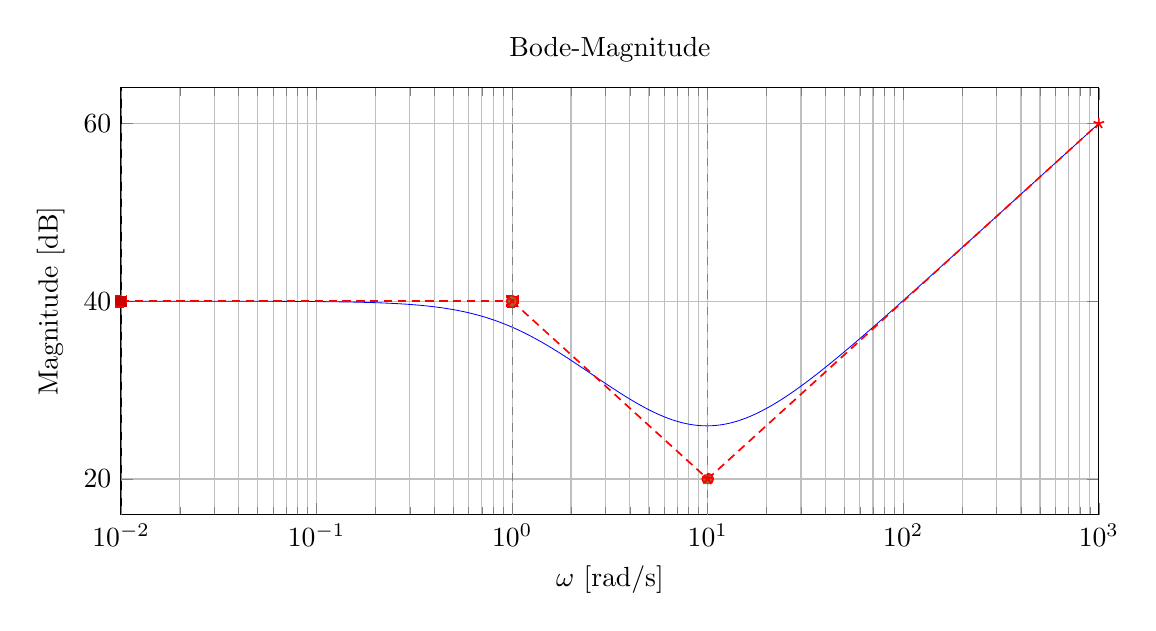
\begin{tikzpicture}
\begin{semilogxaxis}[
  width=14cm,height=7cm,
  xmin=1e-2,xmax=1e3,
  xlabel={$\omega$ [rad/s]},
  ylabel={Magnitude [dB]},
  grid=both,
  ytick distance=20,
  title={Bode-Magnitude}
]
\addplot[
  domain=1e-2:1e3,
  samples=600,
  mark=none,
  line width=0.3pt,
  blue
] {40*ln(sqrt(100 + x^2))/ln(10) - 20*ln(sqrt(1 + x^2))/ln(10)};
\addplot+[domain=1e-2:1,samples=2,dashed,dash pattern=on 3pt off 2pt,line width=0.6pt,red] {40};
\addplot+[domain=1:1e1,samples=2,dashed,dash pattern=on 3pt off 2pt,line width=0.6pt,red] {40 - 20*ln(x)/ln(10)};
\addplot+[domain=1e1:1e3,samples=2,dashed,dash pattern=on 3pt off 2pt,line width=0.6pt,red] {20 + 20*ln(x/10)/ln(10)};
\draw[gray,dashed] (rel axis cs:0,0) -- (rel axis cs:0,1);
\draw[gray,dashed] (axis cs:1,\pgfkeysvalueof{/pgfplots/ymin}) -- (axis cs:1,\pgfkeysvalueof{/pgfplots/ymax});
\draw[gray,dashed] (axis cs:10,\pgfkeysvalueof{/pgfplots/ymin}) -- (axis cs:10,\pgfkeysvalueof{/pgfplots/ymax});
\node[gray,anchor=south east] at (axis cs:1,\pgfkeysvalueof{/pgfplots/ymax}) {\scriptsize Pol $\omega_p=1$};
\node[gray,anchor=south east] at (axis cs:10,\pgfkeysvalueof{/pgfplots/ymax}) {\scriptsize Nullstellen $\omega_z=10$ (LHP \& RHP)};
\end{semilogxaxis}
\end{tikzpicture}
\vspace{6mm}
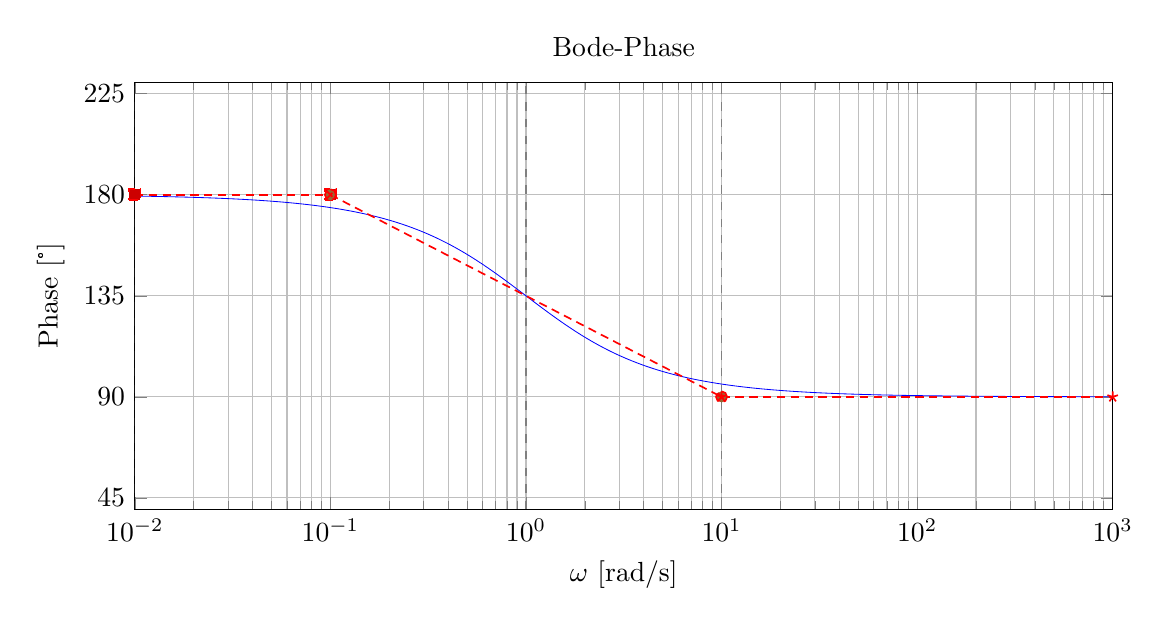
\begin{tikzpicture}
\begin{semilogxaxis}[
  width=14cm,height=7cm,
  xmin=1e-2,xmax=1e3,
  ytick distance=45,
  ymin=40,ymax=230,
  xlabel={$\omega$ [rad/s]},
  ylabel={Phase [°]},
  grid=both,
  title={Bode-Phase}
]
\addplot[
  domain=1e-2:1e3,
  samples=600,
  mark=none,
  line width=0.3pt,
  blue
] {180 - atan(x)};
\addplot+[domain=1e-2:1e-1,samples=2,dashed,dash pattern=on 3pt off 2pt,line width=0.6pt,red] {180};
\addplot+[domain=1e-1:1e1,samples=2,dashed,dash pattern=on 3pt off 2pt,line width=0.6pt,red] {135 - 45*ln(x)/ln(10)};
\addplot+[domain=1e1:1e3,samples=2,dashed,dash pattern=on 3pt off 2pt,line width=0.6pt,red] {90};
\draw[gray,dashed] (rel axis cs:0,0) -- (rel axis cs:0,1);
\draw[gray,dashed] (axis cs:1,\pgfkeysvalueof{/pgfplots/ymin}) -- (axis cs:1,\pgfkeysvalueof{/pgfplots/ymax});
\draw[gray,dashed] (axis cs:10,\pgfkeysvalueof{/pgfplots/ymin}) -- (axis cs:10,\pgfkeysvalueof{/pgfplots/ymax});
\node[gray,anchor=south east] at (axis cs:1,\pgfkeysvalueof{/pgfplots/ymax}) {\scriptsize Pol $\omega_p=1$};
\node[gray,anchor=south east] at (axis cs:10,\pgfkeysvalueof{/pgfplots/ymax}) {\scriptsize Nullstellen $\omega_z=10$ (LHP \& RHP)};
\end{semilogxaxis}
\end{tikzpicture}
\end{center}
\newpage

\subsection{Erklärung (ausführlich)}
\begin{description}[leftmargin=1.2em,labelsep=.6em,font=\bfseries]

\item[1. Normalform herstellen.]
\[
H(s)=\frac{(s-10)(s+10)}{s+1}
=-100\,(1-sT_{z1})\,(1+sT_{z2})\cdot\frac{1}{1+sT_p}
\]
mit
\[
K_0=-100,\quad r=0,\quad T_{z1}=\tfrac{1}{10},\quad T_{z2}=\tfrac{1}{10},\quad T_p=1.
\]
\[
\underline{F}_1(s)=\bigl(1-sT_{z1}\bigr)\ \text{(RHP-Nullstelle)},\]
\[\underline{F}_2(s)=\bigl(1+sT_{z2}\bigr)\ \text{(LHP-Nullstelle)},\]
\[\underline{F}_3(s)=\tfrac{1}{1+sT_p}\ \text{(Pol)}.\]

\item[2. Eckfrequenzen bestimmen und sortieren.]
\[
\omega_{p}=1\,\mathrm{rad/s},\qquad
\omega_{z1}=\omega_{z2}=10\,\mathrm{rad/s},\qquad
\omega_p<\omega_z.
\]

\item[3. Startpunkt des Amplitudengangs festlegen (Geradennäherung).]
Setze \(\omega_{\min}=\omega_p=1\).
\[
F_{\mathrm{dB}}(\omega_{\min})=20\log_{10}\!\big(|K_0\underline{F}_{ges}^*(0)|\,\omega_{\min}^{\,r}\big)=20\log_{10}100=40\,\mathrm{dB}.
\]
Ankerpunkt: \(40\,\mathrm{dB}\) bei \(\omega=1\).

\item[4. Verlauf links vom Startpunkt zeichnen.]
Für \(\omega<1\) horizontale Asymptote bei \(40\,\mathrm{dB}\) (Anfangssteigung \(r\cdot 20\,\mathrm{dB/dec}=0\)). Waagrechte Gerade links von der kleinsten Eckfrequenz eintragen.

\item[5. Steigungswechsel an den Eckfrequenzen eintragen.]
Ab \(\omega=1\): Pol \(\Rightarrow\) Steigungswechsel \(-20\,\mathrm{dB/dec}\).
Ab \(\omega=10\): zwei Nullstellen \(\Rightarrow\) zusätzl. \(+40\,\mathrm{dB/dec}\).
Netto:
\[
\begin{cases}
40\,\mathrm{dB},& \omega<1,\\
40-20\log_{10}\omega,& 1\le\omega<10,\\
20+20\log_{10}(\omega/10),& \omega\ge 10.
\end{cases}
\]

\item[6. Eckabrundungen korrekt berücksichtigen.]
Einfacher Pol bei \(\omega=1\): \(-3\,\mathrm{dB}\) am Knick \(\Rightarrow |H(j1)|_{\mathrm{dB}}\approx 40-3=37\,\mathrm{dB}\).
Zwei Nullstellen bei \(\omega=10\): \(+6\,\mathrm{dB}\) am Knick \(\Rightarrow |H(j10)|_{\mathrm{dB}}\approx 20+6=26\,\mathrm{dB}\).

\item[7. Phasenstartwert festlegen.]
Verwende die Regel für $K_0\underline{F}_{ges}^*(0) <0$:
\[
\varphi(0)=-180^\circ + r\cdot 90^\circ= -180^\circ
\]
(Darstellung im Plot um \(+360^\circ\) verschoben \(\Rightarrow\) Start bei \(+180^\circ\)).

\item[8. Phasenänderung durch Pol und Nullstellen eintragen.]
Pol bei \(\omega_p\) bewirkt eine Phasenänderung \(-90^\circ\) über \([0.1,10]\).
Nullstellen bei \(\omega_z\): LHP-Nullstelle \(+90^\circ\) und RHP-Nullstelle \(-90^\circ\), beide über \([1,100]\). die \(+90^\circ\) und \(-90^\circ\) der beiden Nullstellen kompensieren sich zu \(0^\circ\). Netto wirkt in $[1,10]$ nur der Pol.
Näherung (mit Phasenverschiebung um \(+360^\circ\) gezeigt):
\[
\varphi(\omega)\approx
\begin{cases}
180^\circ,& \omega\le 0.1,\\
135^\circ-45^\circ\log_{10}\omega,& 0.1<\omega<10,\\
90^\circ,& \omega\ge 10.
\end{cases}
\]

\item[9. Grenzwerte und Konsistenz prüfen.]
DC: \(|H(0)|=100\Rightarrow 40\,\mathrm{dB}\); \(\varphi(0)=-180^\circ\) (gezeigt als \(+180^\circ\)).
HF: \(|H(j\omega)|\sim \omega^2/\omega= \omega \Rightarrow 20\log_{10}\omega + 20\,\mathrm{dB}\).

\end{description}

\subsubsection*{Stückweise Näherungen (für die Skizze)}
\[
|H(j\omega)|_{\mathrm{dB}}\approx
\begin{cases}
40,& \omega\ll 1,\\[2pt]
40-3,& \omega=1,\\[2pt]
40-20\log_{10}\omega,& 1\ll\omega\ll 10,\\[2pt]
20+6,& \omega=10,\\[2pt]
20+20\log_{10}(\omega/10),& \omega\gg 10,
\end{cases}
\]
\[
\varphi(\omega)\ (\text{Darstellung }+360^\circ)\approx
\begin{cases}
180^\circ,& \omega\le 0.1,\\[2pt]
135^\circ-45^\circ\log_{10}\omega,& 0.1<\omega<10,\\[2pt]
90^\circ,& \omega\ge 10.
\end{cases}
\]

\newpage
\section{}
\[
H(s)=\frac{10\sqrt{202}\,s}{(s+1)(s+10)}\,.
\]
\subsection{Bode-Diagramm}
\begin{center}
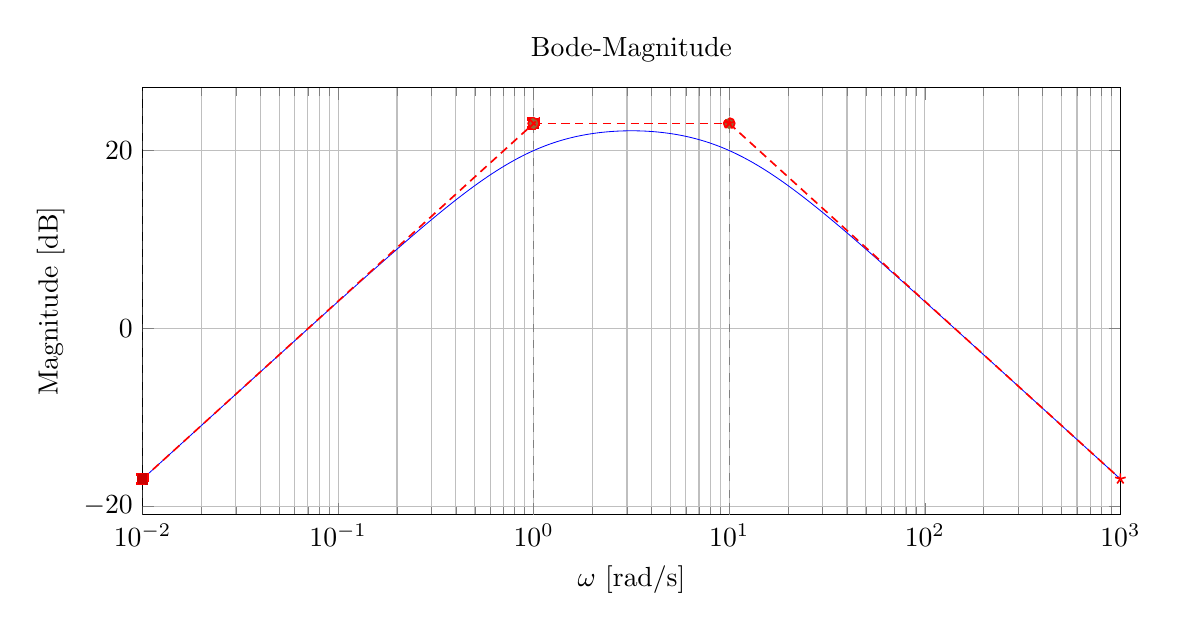
\begin{tikzpicture}
\begin{semilogxaxis}[
  width=14cm,height=7cm,
  xmin=1e-2,xmax=1e3,
  xlabel={$\omega$ [rad/s]},
  ylabel={Magnitude [dB]},
  ytick distance=20,
  grid=both,
  title={Bode-Magnitude}
]
\addplot[
  domain=1e-2:1e3,
  samples=600,
  mark=none,
  line width=0.3pt,
  blue
] {20 + 10*ln(202)/ln(10) + 20*ln(x)/ln(10) - 20*ln(sqrt(1 + x^2))/ln(10) - 20*ln(sqrt(100 + x^2))/ln(10)};
\addplot+[domain=1e-2:1,samples=2,dashed,dash pattern=on 3pt off 2pt,line width=0.6pt,red] {10*ln(202)/ln(10) + 20*ln(x)/ln(10)};
\addplot+[domain=1:1e1,samples=2,dashed,dash pattern=on 3pt off 2pt,line width=0.6pt,red] {10*ln(202)/ln(10)};
\addplot+[domain=1e1:1e3,samples=2,dashed,dash pattern=on 3pt off 2pt,line width=0.6pt,red] {10*ln(202)/ln(10) - 20*ln(x/10)/ln(10)};
\draw[gray,dashed] (rel axis cs:0,0) -- (rel axis cs:0,1);
\draw[gray,dashed] (axis cs:1,\pgfkeysvalueof{/pgfplots/ymin}) -- (axis cs:1,\pgfkeysvalueof{/pgfplots/ymax});
\draw[gray,dashed] (axis cs:10,\pgfkeysvalueof{/pgfplots/ymin}) -- (axis cs:10,\pgfkeysvalueof{/pgfplots/ymax});
\node[gray,anchor=south east] at (axis cs:1,\pgfkeysvalueof{/pgfplots/ymax}) {\scriptsize Pol $\omega_{p1}=1$};
\node[gray,anchor=south east] at (axis cs:10,\pgfkeysvalueof{/pgfplots/ymax}) {\scriptsize Pol $\omega_{p2}=10$};
\end{semilogxaxis}
\end{tikzpicture}
\vspace{6mm}
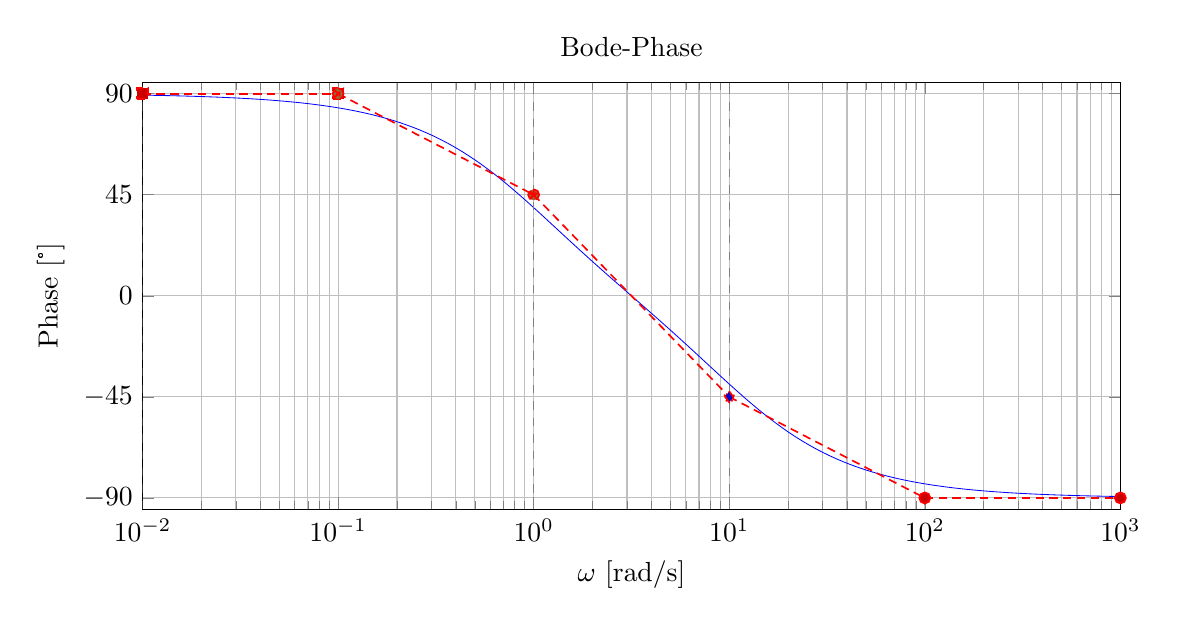
\begin{tikzpicture}
\begin{semilogxaxis}[
  width=14cm,height=7cm,
  xmin=1e-2,xmax=1e3,
  ymin=-95,ymax=95,
  ytick distance=45,
  xlabel={$\omega$ [rad/s]},
  ylabel={Phase [°]},
  grid=both,
  title={Bode-Phase}
]
\addplot[
  domain=1e-2:1e3,
  samples=600,
  mark=none,
  line width=0.3pt,
  blue
] {90 - atan(x) - atan(x/10)};
\addplot+[domain=1e-2:1e-1,samples=2,dashed,dash pattern=on 3pt off 2pt,line width=0.6pt,red] {90};
\addplot+[domain=1e-1:1e0,samples=2,dashed,dash pattern=on 3pt off 2pt,line width=0.6pt,red] {45 - 45*ln(x)/ln(10)};
\addplot+[domain=1e0:1e1,samples=2,dashed,dash pattern=on 3pt off 2pt,line width=0.6pt,red]{45 - 90*ln(x)/ln(10)};
\addplot+[domain=1e1:1e2,samples=2,dashed,dash pattern=on 3pt off 2pt,line width=0.6pt,red]{-45 - 45*ln(x/10)/ln(10)}; % bei 10: -45°, bei 100: -90°

\addplot+[domain=1e2:1e3,samples=2,dashed,dash pattern=on 3pt off 2pt,line width=0.6pt,red] {-90};
\draw[gray,dashed] (rel axis cs:0,0) -- (rel axis cs:0,1);
\draw[gray,dashed] (axis cs:1,\pgfkeysvalueof{/pgfplots/ymin}) -- (axis cs:1,\pgfkeysvalueof{/pgfplots/ymax});
\draw[gray,dashed] (axis cs:10,\pgfkeysvalueof{/pgfplots/ymin}) -- (axis cs:10,\pgfkeysvalueof{/pgfplots/ymax});
\node[gray,anchor=south east] at (axis cs:1,\pgfkeysvalueof{/pgfplots/ymax}) {\scriptsize Pol $\omega_{p1}=1$};
\node[gray,anchor=south east] at (axis cs:10,\pgfkeysvalueof{/pgfplots/ymax}) {\scriptsize Pol $\omega_{p2}=10$};
\end{semilogxaxis}
\end{tikzpicture}
\end{center}
\newpage
\subsection{Erklärung}
\vspace{5mm}
\begin{description}[leftmargin=1.2em,labelsep=.6em,font=\bfseries]
\item[Schritt 1] Nullstelle im Ursprung: $H(s)=10\sqrt{202}\,\dfrac{s}{(s+1)(s+10)}$. Für $\omega\ll1$ gilt $|H(\j\omega)|\approx \sqrt{202}\,\omega$; Startsteigung $+20\,\mathrm{dB/dec}$ mit Fixniveau\footnote{Die Festlegung der ersten Geradennäherung gestaltet sich hier schwierig. Alternativ kann man die Verstärkung bei der Eckfrequenz $\omega=1$ ansetzen; dabei ist zu beachten, dass man den exakten Wert der blauen Kurve berechnet und dieser etwa $3\,\mathrm{dB}$ unter der Geradennäherung liegt, welche man dann einzeichnen muss.}$10\log_{10}202\,\mathrm{dB} = 23\,\mathrm{dB}$ bei $\omega = 5$. Startphase $\approx+90^\circ$.
\item[Schritt 2] Pol bei $\omega_{p1}=1\,\mathrm{rad/s}$: ab $\omega=1$ Steigungswechsel um $-20\,\mathrm{dB/dec}$; Zwischenbereich $[1,10]$ ist betragsflach. Exakt $|H(\j1)|=\dfrac{10\sqrt{202}}{\sqrt{2}\sqrt{101}}=10\Rightarrow20\,\mathrm{dB}$ (symmetrische Ecklage). Phasenabfall um $90^\circ$ über $\omega\in[0.1,10]$; Geradennäherung $45^\circ-45^\circ\log_{10}\omega$.
\item[Schritt 3] Pol bei $\omega_{p2}=10\,\mathrm{rad/s}$: ab $\omega=10$ weiterer Steigungswechsel um $-20\,\mathrm{dB/dec}$; Gesamtslope $\,-20\,\mathrm{dB/dec}$ für $\omega\gg10$. Auch hier $|H(\j10)|=\dfrac{100\sqrt{202}}{\sqrt{101}\sqrt{200}}=10\Rightarrow20\,\mathrm{dB}$. Der zweite Pol senkt die Phase um weitere $90^\circ$ in $\omega\in[1,100]$; Geradennäherung $-45^\circ\log_{10}(\omega/10)$, Grenzwert $\angle H\to-90^\circ$.
\end{description}

\vspace{0.5cm}
\medskip
\noindent\textbf{Stückweise Näherung}
\[
|H(\j\omega)|_{\mathrm{dB}}\approx
\begin{cases}
10\log_{10}202+20\log_{10}\omega,& \omega\ll1,\\[4pt]
20,& \omega=1,\\[4pt]
10\log_{10}202,& 1\ll\omega\ll10,\\[4pt]
20,& \omega=10,\\[4pt]
10\log_{10}202-20\log_{10}(\omega/10),& \omega\gg10,
\end{cases}
\qquad
\]
\newpage
\section{}
\[
H(s)=\frac{s\,(0.1 - s)\,(s+10)}{(s+1)^2}\,.
\]
\subsection{Bode-Diagramm}
\begin{center}
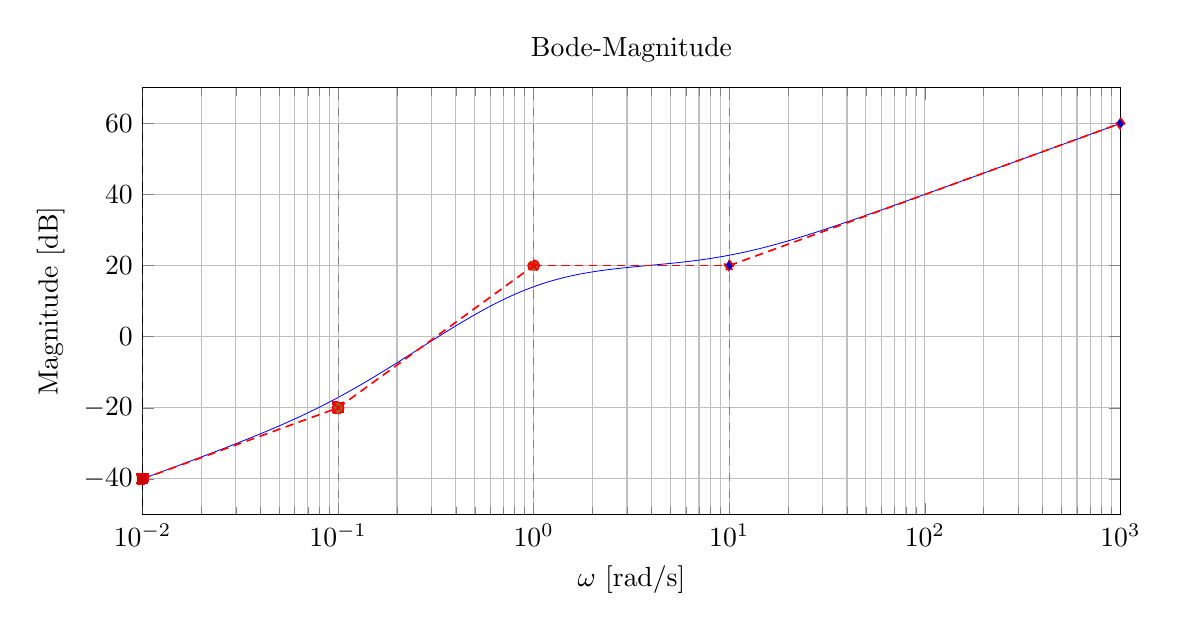
\begin{tikzpicture}
\begin{semilogxaxis}[
  width=14cm,height=7cm,
  ytick distance=20,
  xmin=1e-2,xmax=1e3,
  xlabel={$\omega$ [rad/s]},
  ylabel={Magnitude [dB]},
  grid=both,
  title={Bode-Magnitude}
]
\addplot[
  domain=1e-2:1e3,
  samples=800,
  mark=none,
  line width=0.3pt,
  blue
] {20*ln(x)/ln(10)
   +20*ln(sqrt(1 + (x/0.1)^2))/ln(10)
   +20*ln(sqrt(1 + (x/10)^2))/ln(10)
   -40*ln(sqrt(1 + x^2))/ln(10)};
\addplot+[domain=1e-2:1e-1,samples=2,dashed,dash pattern=on 3pt off 2pt,line width=0.6pt,red] {20*ln(x)/ln(10)};
\addplot+[domain=1e-1:1,samples=2,dashed,dash pattern=on 3pt off 2pt,line width=0.6pt,red] {40*ln(x)/ln(10) + 20};
\addplot+[domain=1:1e1,samples=2,dashed,dash pattern=on 3pt off 2pt,line width=0.6pt,red] {20};
\addplot+[domain=1e1:1e3,samples=2,dashed,dash pattern=on 3pt off 2pt,line width=0.6pt,red] {20 + 20*ln(x/10)/ln(10)};
\draw[gray,dashed] (rel axis cs:0,0) -- (rel axis cs:0,1);
\draw[gray,dashed] (axis cs:0.1,\pgfkeysvalueof{/pgfplots/ymin}) -- (axis cs:0.1,\pgfkeysvalueof{/pgfplots/ymax});
\draw[gray,dashed] (axis cs:1,\pgfkeysvalueof{/pgfplots/ymin}) -- (axis cs:1,\pgfkeysvalueof{/pgfplots/ymax});
\draw[gray,dashed] (axis cs:10,\pgfkeysvalueof{/pgfplots/ymin}) -- (axis cs:10,\pgfkeysvalueof{/pgfplots/ymax});
\node[gray,anchor=south east] at (axis cs:0.1,\pgfkeysvalueof{/pgfplots/ymax}) {\scriptsize Nullstelle $\omega_z=0.1$ (RHP)};
\node[gray,anchor=south east] at (axis cs:1,\pgfkeysvalueof{/pgfplots/ymax}) {\scriptsize Pol $\omega_p=1$ (doppelt)};
\node[gray,anchor=south east] at (axis cs:10,\pgfkeysvalueof{/pgfplots/ymax}) {\scriptsize Nullstelle $\omega_z=10$};
\end{semilogxaxis}
\end{tikzpicture}
\vspace{6mm}
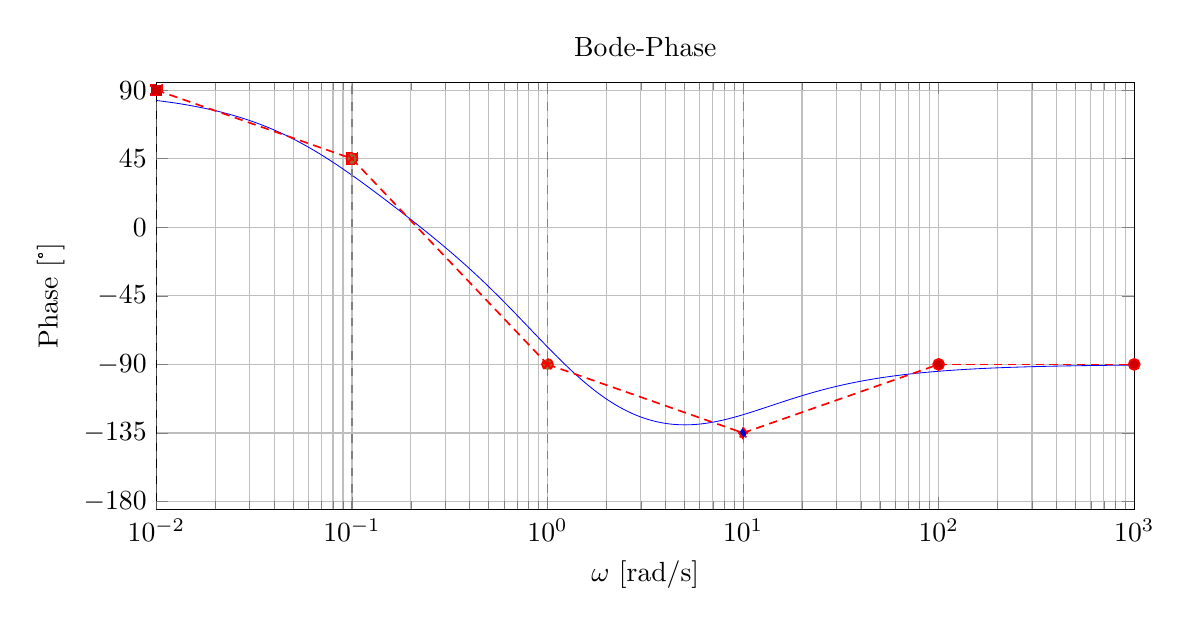
\begin{tikzpicture}
\begin{semilogxaxis}[
  width=14cm,height=7cm,
  xmin=1e-2,xmax=1e3,
  ytick distance=45,
  ymin=-185,ymax=95,
  xlabel={$\omega$ [rad/s]},
  ylabel={Phase [°]},
  grid=both,
  title={Bode-Phase}
]
\addplot[
  domain=1e-2:1e3,
  samples=800,
  mark=none,
  line width=0.3pt,
  blue
] {90 - atan(x/0.1) + atan(x/10) - 2*atan(x)};
\addplot+[domain=1e-2:1e-1,samples=2,dashed,dash pattern=on 3pt off 2pt,line width=0.6pt,red] {45 - 45*ln(x/0.1)/ln(10)};
\addplot+[domain=1e-1:1e0,samples=2,dashed,dash pattern=on 3pt off 2pt,line width=0.6pt,red] {45 - 135*ln(x/0.1)/ln(10)};
\addplot+[domain=1e0:1e1,samples=2,dashed,dash pattern=on 3pt off 2pt,line width=0.6pt,red] {-90 - 45*ln(x)/ln(10)};
\addplot+[domain=1e1:1e2,samples=2,dashed,dash pattern=on 3pt off 2pt,line width=0.6pt,red] {-135 + 45*ln(x/10)/ln(10)};
\addplot+[domain=1e2:1e3,samples=2,dashed,dash pattern=on 3pt off 2pt,line width=0.6pt,red] {-90};
\draw[gray,dashed] (rel axis cs:0,0) -- (rel axis cs:0,1);
\draw[gray,dashed] (axis cs:0.1,\pgfkeysvalueof{/pgfplots/ymin}) -- (axis cs:0.1,\pgfkeysvalueof{/pgfplots/ymax});
\draw[gray,dashed] (axis cs:1,\pgfkeysvalueof{/pgfplots/ymin}) -- (axis cs:1,\pgfkeysvalueof{/pgfplots/ymax});
\draw[gray,dashed] (axis cs:10,\pgfkeysvalueof{/pgfplots/ymin}) -- (axis cs:10,\pgfkeysvalueof{/pgfplots/ymax});
\node[gray,anchor=south east] at (axis cs:0.1,\pgfkeysvalueof{/pgfplots/ymax}) {\scriptsize Nullstelle $\omega_z=0.1$ (RHP)};
\node[gray,anchor=south east] at (axis cs:1,\pgfkeysvalueof{/pgfplots/ymax}) {\scriptsize Pol $\omega_p=1$ (doppelt)};
\node[gray,anchor=south east] at (axis cs:10,\pgfkeysvalueof{/pgfplots/ymax}) {\scriptsize Nullstelle $\omega_z=10$};
\end{semilogxaxis}
\end{tikzpicture}
\end{center}
\newpage
\subsection{Erklärung}
\vspace{5mm}
\begin{description}[leftmargin=1.2em,labelsep=.6em,font=\bfseries]
\item[Schritt 1] Struktur und Startverhalten: $H(s)=\dfrac{s(0.1-s)(s+10)}{(s+1)^2}$. Für $\omega\ll0.1$ gilt $|H(\j\omega)|\approx \omega\cdot 0.1\cdot 10/1=\omega$ $\Rightarrow$ Startsteigung $+20\,\mathrm{dB/dec}$; Startphase aus $\j\omega$ ist $\approx+90^\circ$ (keine Übergänge aktiv).
\item[Schritt 2] RHP-Nullstelle bei $\omega_z=0.1\,\mathrm{rad/s}$: Magnitude-Beitrag wie LHP-Nullstelle $\Rightarrow$ zusätzlicher Anstieg $+20\,\mathrm{dB/dec}$ ab $\omega=0.1$; Phase hingegen fällt nicht-minimumphasig um $90^\circ$ über $\omega\in[0.01,1]$ (Geradennäherung: $45^\circ-45^\circ\log_{10}(\omega/0.1)$ bis $45^\circ-135^\circ\log_{10}(\omega/0.1)$).
\item[Schritt 3] Doppelpol bei $\omega_p=1\,\mathrm{rad/s}$ und LHP-Nullstelle bei $\omega_z=10\,\mathrm{rad/s}$: Der Doppelpol reduziert die Slope um $-40\,\mathrm{dB/dec}$ $\Rightarrow$ Netto $0\,\mathrm{dB/dec}$ in $[1,10]$ (Betrag $\approx20\,\mathrm{dB}$ als Geraden-Niveau); die LHP-Nullstelle hebt ab $\omega=10$ die Slope wieder auf $+20\,\mathrm{dB/dec}$. Phasenbild: der Doppelpol liefert insgesamt $-180^\circ$ über $\omega\in[0.1,10]$; die LHP-Nullstelle addiert $+90^\circ$ über $\omega\in[1,100]$. Daraus resultieren die roten Segmente: $+90^\circ\to+45^\circ$ ($[0.01,0.1]$), weiter bis $\approx-90^\circ$ ($[0.1,1]$), in $[1,10]$ Abfall bis $\approx-135^\circ$, anschließend Anstieg zurück gegen $\approx-90^\circ$ für $\omega\gg100$.
\end{description}

\vspace{0.5cm}
\medskip
\noindent\textbf{Stückweise Näherung}
\[
|H(\j\omega)|_{\mathrm{dB}}\approx
\begin{cases}
20\log_{10}\omega,& \omega\ll0.1,\\[4pt]
40\log_{10}\omega+20,& 0.1\ll\omega\ll1,\\[4pt]
20,& 1\ll\omega\ll10,\\[4pt]
20+20\log_{10}(\omega/10),& \omega\gg10,
\end{cases}
\qquad
\]
\newpage
\section{}
\[
H(s)=\frac{1}{s}\,.
\]
\subsection{Bode-Diagramm}
\begin{center}
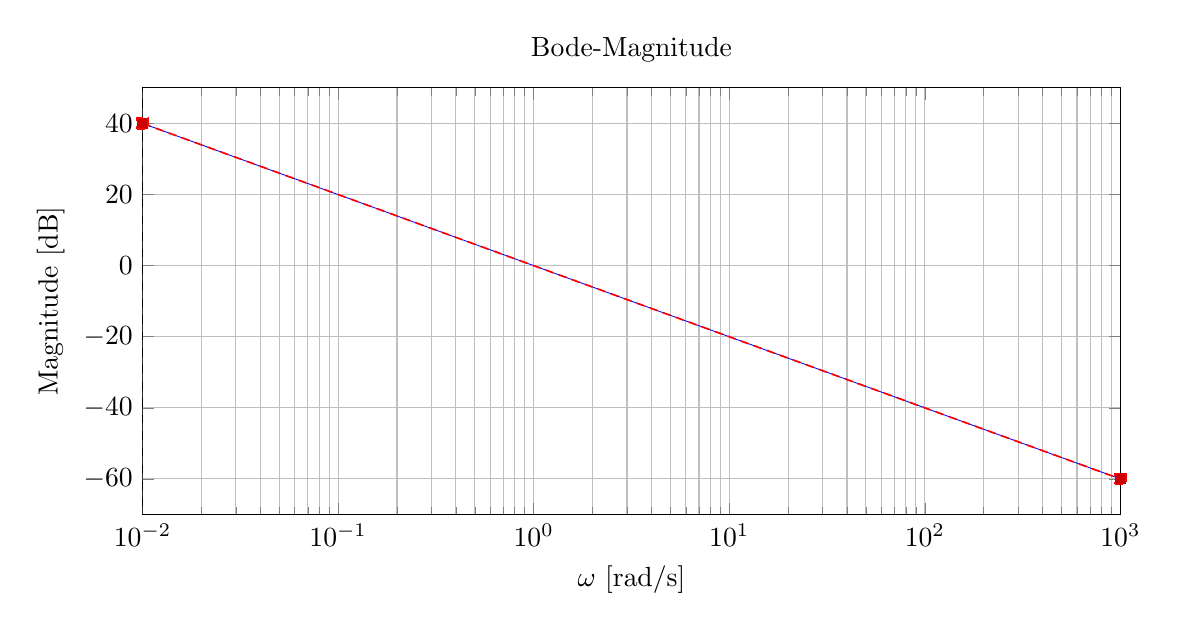
\begin{tikzpicture}
\begin{semilogxaxis}[
  width=14cm,height=7cm,
  ytick distance=20,
  xmin=1e-2,xmax=1e3,
  xlabel={$\omega$ [rad/s]},
  ylabel={Magnitude [dB]},
  grid=both,
  title={Bode-Magnitude}
]
\addplot[
  domain=1e-2:1e3,
  samples=400,
  mark=none,
  line width=0.3pt,
  blue
] {-20*ln(x)/ln(10)};
\addplot+[domain=1e-2:1e3,samples=2,dashed,dash pattern=on 3pt off 2pt,line width=0.6pt,red] {-20*ln(x)/ln(10)};
\draw[gray,dashed] (rel axis cs:0,0) -- (rel axis cs:0,1);
\end{semilogxaxis}
\end{tikzpicture}
\vspace{6mm}
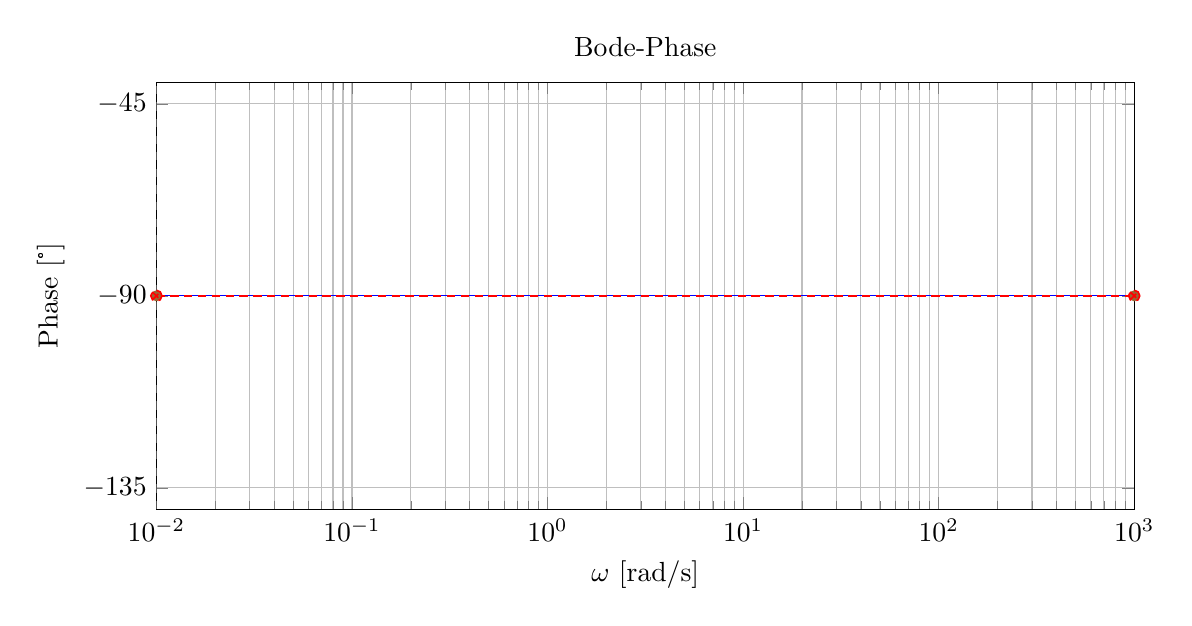
\begin{tikzpicture}
\begin{semilogxaxis}[
  width=14cm,height=7cm,
  xmin=1e-2,xmax=1e3,
  ymin=-140,ymax=-40,
  ytick distance=45,
  xlabel={$\omega$ [rad/s]},
  ylabel={Phase [°]},
  grid=both,
  title={Bode-Phase}
]
\addplot[
  domain=1e-2:1e-3,
  samples=2,
  mark=none,
  line width=0.3pt,
  blue
] {-90};
\addplot[
  domain=1e-3:1e3,
  samples=2,
  mark=none,
  line width=0.3pt,
  blue
] {-90};
\addplot+[domain=1e-2:1e3,samples=2,dashed,dash pattern=on 3pt off 2pt,line width=0.6pt,red] {-90};
\draw[gray,dashed] (rel axis cs:0,0) -- (rel axis cs:0,1);
\end{semilogxaxis}
\end{tikzpicture}
\end{center}
\newpage
\subsection{Erklärung}
\vspace{5mm}
\begin{description}[leftmargin=1.2em,labelsep=.6em,font=\bfseries]
\item[Schritt 1] Pol im Ursprung: $H(s)=1/s$ liefert für alle $\omega>0$ die Betragsasymptote $|H(\j\omega)|_{\mathrm{dB}}=-20\log_{10}\omega$ mit konstanter Steigung $-20\,\mathrm{dB/dec}$; keine endliche Eckfrequenz. Wir benötigen ein Fixpunkt und wählen diesen beliebig bei $\omega = 1$ $\rightarrow$ $|H(1)|_{dB} = 20 log_{10}(1)\,\mathrm{dB} = 0\,\mathrm{dB}$
\item[Schritt 2] Phase: $\angle(1/\j\omega)=-90^\circ$ für alle Frequenzen; keine Übergangsdekaden, daher rote Geradennäherung deckungsgleich mit dem exakten Verlauf.
\item[Schritt 3] Grenzfälle: $\omega\to0^+$ $\Rightarrow$ $|H|\to\infty$ (Integrator), $\omega\to\infty$ $\Rightarrow$ $|H|\to0$; Phase bleibt stets $-90^\circ$.
\end{description}

\vspace{0.5cm}
\medskip
\noindent\textbf{Stückweise Näherung}
\[
|H(\j\omega)|_{\mathrm{dB}}\approx
\begin{cases}
-20\log_{10}\omega,& \omega\ll1,\\[4pt]
0,& \omega=1,\\[4pt]
-20\log_{10}\omega,& \omega\gg1,
\end{cases}
\qquad
\]
\newpage
\section{}
\[
H(s)=\frac{100}{s^2+s+100}\,.
\]
\subsection{Bode-Diagramm}
\begin{center}
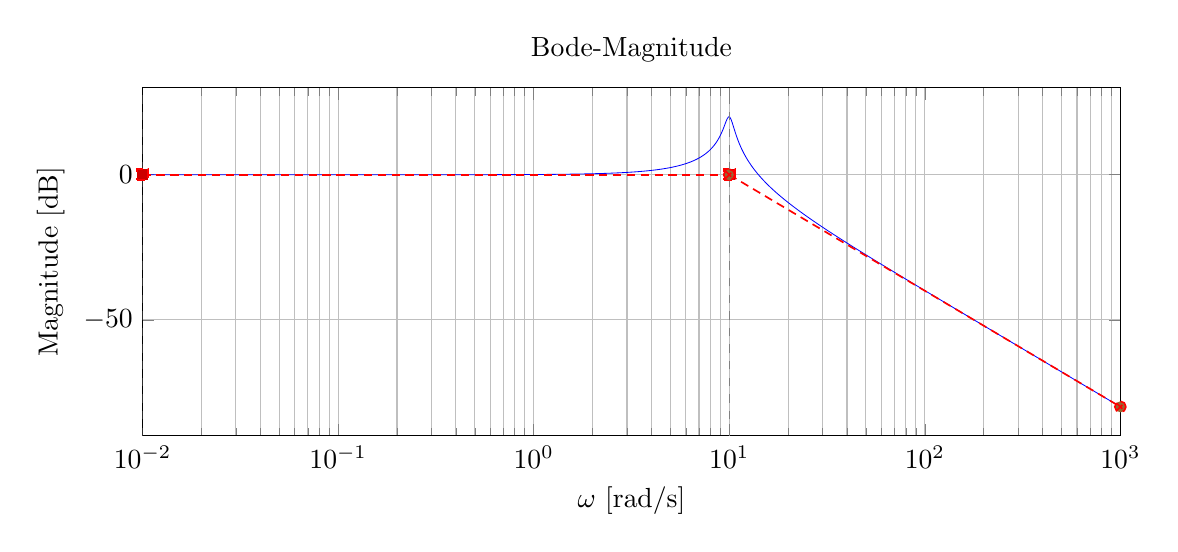
\begin{tikzpicture}
\begin{semilogxaxis}[
  width=14cm,height=6cm,
  xmin=1e-2,xmax=1e3,
  xlabel={$\omega$ [rad/s]},
  ylabel={Magnitude [dB]},
  grid=both,
  title={Bode-Magnitude}
]
\addplot[
  domain=1e-2:1e3,
  samples=800,
  mark=none,
  line width=0.3pt,
  blue
] {-10*ln((1 - (x/10)^2)^2 + (x/100)^2)/ln(10)};
\addplot+[domain=1e-2:1e1,samples=2,dashed,dash pattern=on 3pt off 2pt,line width=0.6pt,red] {0};
\addplot+[domain=1e1:1e3,samples=2,dashed,dash pattern=on 3pt off 2pt,line width=0.6pt,red] {-40*ln(x/10)/ln(10)};
\draw[gray,dashed] (rel axis cs:0,0) -- (rel axis cs:0,1);
\draw[gray,dashed] (axis cs:10,\pgfkeysvalueof{/pgfplots/ymin}) -- (axis cs:10,\pgfkeysvalueof{/pgfplots/ymax});
\node[gray,anchor=south east] at (axis cs:10,\pgfkeysvalueof{/pgfplots/ymax}) {\scriptsize Polpaar $\omega_n=10$, $\zeta=0.05$};
\end{semilogxaxis}
\end{tikzpicture}
\vspace{6mm}
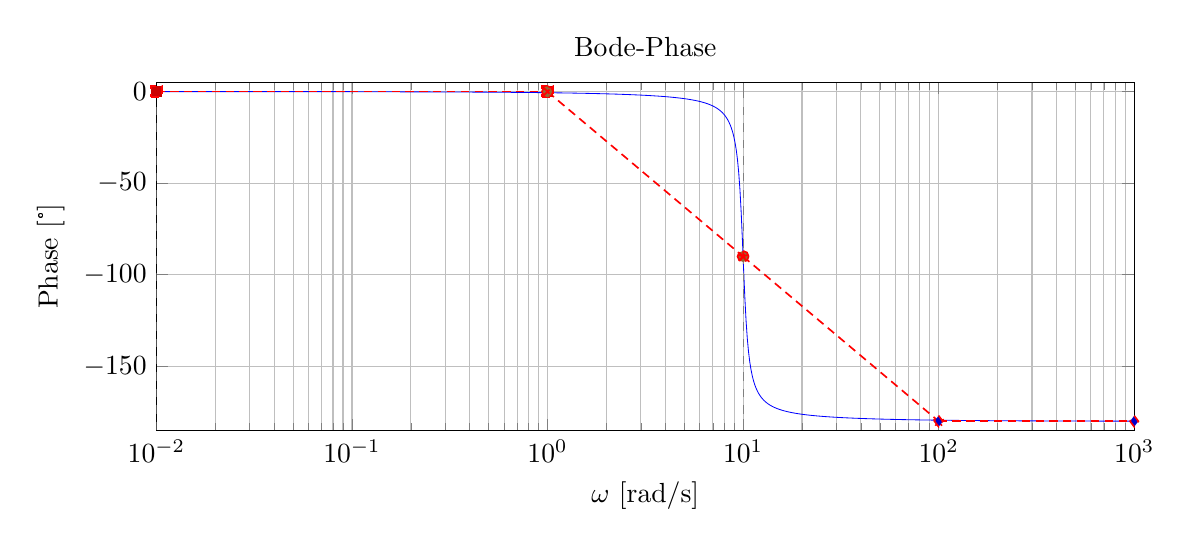
\begin{tikzpicture}
\begin{semilogxaxis}[
  width=14cm,height=6cm,
  xmin=1e-2,xmax=1e3,
  ymin=-185,ymax=5,
  xlabel={$\omega$ [rad/s]},
  ylabel={Phase [°]},
  grid=both,
  title={Bode-Phase}
]
\addplot[
  domain=1e-2:1e3,
  samples=800,
  mark=none,
  line width=0.3pt,
  blue
] {-atan2(x/100, 1 - (x/10)^2)};
\addplot+[domain=1e-2:1e0,samples=2,dashed,dash pattern=on 3pt off 2pt,line width=0.6pt,red] {0};
\addplot+[domain=1e0:1e1,samples=2,dashed,dash pattern=on 3pt off 2pt,line width=0.6pt,red] {-90*ln(x)/ln(10)};
\addplot+[domain=1e1:1e2,samples=2,dashed,dash pattern=on 3pt off 2pt,line width=0.6pt,red] {-90 - 90*ln(x/10)/ln(10)};
\addplot+[domain=1e2:1e3,samples=2,dashed,dash pattern=on 3pt off 2pt,line width=0.6pt,red] {-180};
\draw[gray,dashed] (rel axis cs:0,0) -- (rel axis cs:0,1);
\draw[gray,dashed] (axis cs:10,\pgfkeysvalueof{/pgfplots/ymin}) -- (axis cs:10,\pgfkeysvalueof{/pgfplots/ymax});
\node[gray,anchor=south east] at (axis cs:10,\pgfkeysvalueof{/pgfplots/ymax}) {\scriptsize Polpaar $\omega_n=10$, $\zeta=0.05$};
\end{semilogxaxis}
\end{tikzpicture}
\end{center}
\newpage
\subsection{Erklärung}
\vspace{5mm}
\begin{description}[leftmargin=1.2em,labelsep=.6em,font=\bfseries]
\item[Schritt 1] Normform: $s^2+s+100=\omega_n^2\!\left[\left(\tfrac{s}{\omega_n}\right)^2+2\zeta\left(\tfrac{s}{\omega_n}\right)+1\right]$ mit $\omega_n=10$ und $\zeta=\tfrac{1}{2\omega_n}=0.05$. DC-Faktor $100/100=1\Rightarrow 0\,\mathrm{dB}$ ohne Anfangssteigung; Startphase $\approx0^\circ$.
\item[Schritt 2] Konjugiertes Polpaar: Break bei $\omega_n=10$. Asymptote $0\,\mathrm{dB}$ für $\omega\ll10$, ab $\omega=10$ Slope $-40\,\mathrm{dB/dec}$. Exakt liegt am Eigenkreis die Verstärkung bei $|H(\j\omega_n)|=\tfrac{1}{2\zeta}=10\Rightarrow20\,\mathrm{dB}$ (ausgeprägte Resonanzspitze wegen kleiner $\zeta$).
\item[Schritt 3] Phase: Gesamtabfall um $180^\circ$ um $\omega_n$, für die Geradennäherung über zwei Dekaden verteilt ($[1,100]$): $0^\circ\to-90^\circ$ in $[1,10]$, weiter $-90^\circ\to-180^\circ$ in $[10,100]$. Für $\omega\gg10$ nähert sich $|H|\sim \omega^{-2}$ und $\angle H\to-180^\circ$.
\end{description}

\vspace{0.5cm}
\medskip
\noindent\textbf{Stückweise Näherung}
\[
|H(\j\omega)|_{\mathrm{dB}}\approx
\begin{cases}
0,& \omega\ll10,\\[4pt]
+20,& \omega=10,\\[4pt]
-40\log_{10}(\omega/10),& \omega\gg10,
\end{cases}
\qquad
\]
\newpage
\section{}
\[
H(s)=\frac{s^2+4}{s\,(s^2+10s+100)}\,.
\]
\subsection{Bode-Diagramm}
\begin{center}
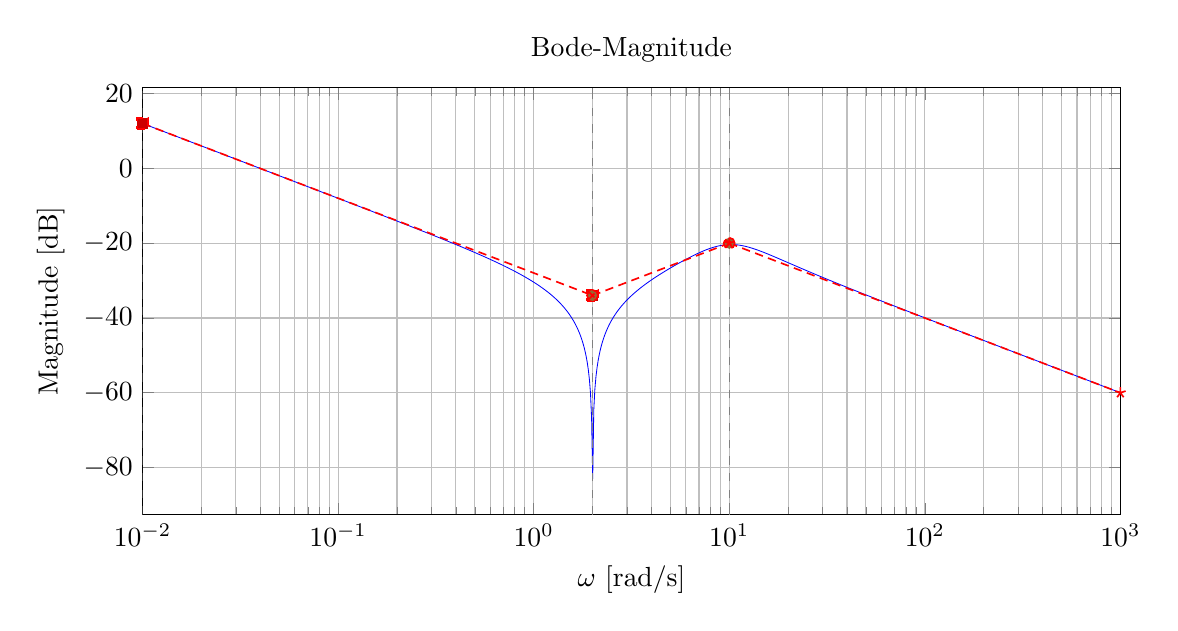
\begin{tikzpicture}
\begin{semilogxaxis}[
  width=14cm,height=7cm,
  xmin=1e-2,xmax=1e3,
  ytick distance=20,
  xlabel={$\omega$ [rad/s]},
  ylabel={Magnitude [dB]},
  grid=both,
  title={Bode-Magnitude}
]
\addplot[
  domain=1e-2:1e3,
  samples=900,
  mark=none,
  line width=0.3pt,
  blue
] {20*ln(abs(4 - x^2))/ln(10) - 20*ln(x)/ln(10) - 10*ln((100 - x^2)^2 + (10*x)^2)/ln(10)};
\addplot+[domain=1e-2:2,samples=2,dashed,dash pattern=on 3pt off 2pt,line width=0.6pt,red] {20*ln(0.04)/ln(10) - 20*ln(x)/ln(10)};
\addplot+[domain=2:1e1,samples=2,dashed,dash pattern=on 3pt off 2pt,line width=0.6pt,red] {-40 + 20*ln(x)/ln(10)};
\addplot+[domain=1e1:1e3,samples=2,dashed,dash pattern=on 3pt off 2pt,line width=0.6pt,red] {-20 - 20*ln(x/10)/ln(10)};
\draw[gray,dashed] (rel axis cs:0,0) -- (rel axis cs:0,1);
\draw[gray,dashed] (axis cs:2,\pgfkeysvalueof{/pgfplots/ymin}) -- (axis cs:2,\pgfkeysvalueof{/pgfplots/ymax});
\draw[gray,dashed] (axis cs:10,\pgfkeysvalueof{/pgfplots/ymin}) -- (axis cs:10,\pgfkeysvalueof{/pgfplots/ymax});
\node[gray,anchor=south east] at (axis cs:2,\pgfkeysvalueof{/pgfplots/ymax}) {\scriptsize Doppelnullstellen $\omega_z=2$ (j-Achse)};
\node[gray,anchor=south east] at (axis cs:10,\pgfkeysvalueof{/pgfplots/ymax}) {\scriptsize Polpaar $\omega_n=10$, $\zeta=0.5$};
\end{semilogxaxis}
\end{tikzpicture}
\vspace{6mm}
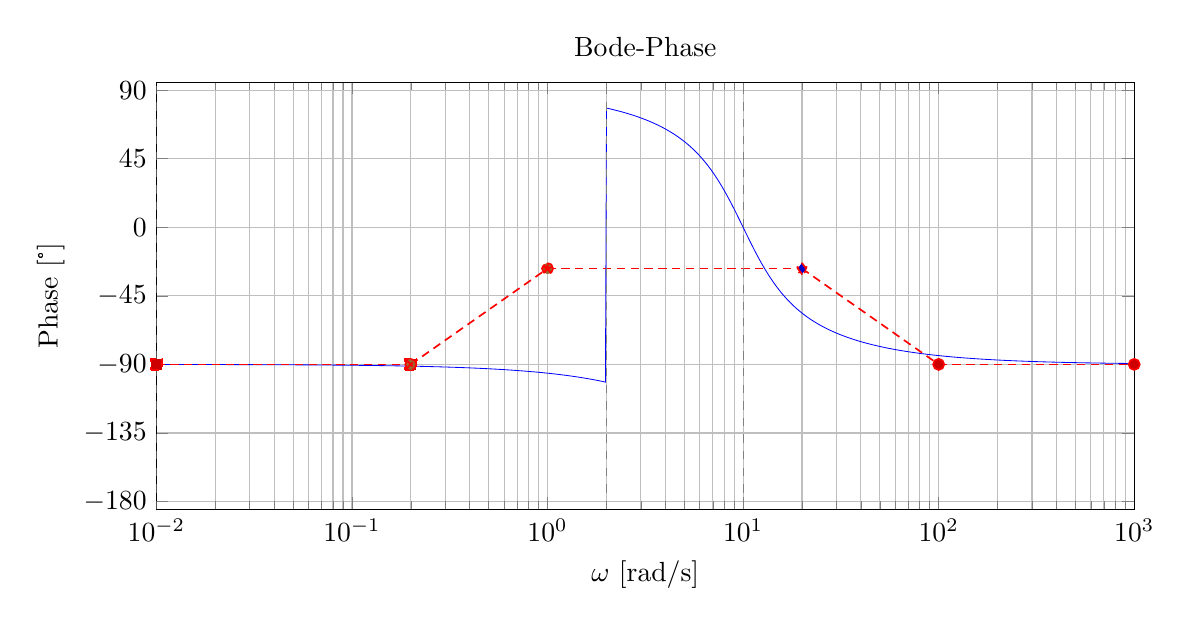
\begin{tikzpicture}
\begin{semilogxaxis}[
  width=14cm,height=7cm,
  xmin=1e-2,xmax=1e3,
  ytick distance=45,
  ymin=-185,ymax=95,
  xlabel={$\omega$ [rad/s]},
  ylabel={Phase [°]},
  grid=both,
  title={Bode-Phase}
]
\addplot[
  domain=1e-2:1e3,
  samples=900,
  mark=none,
  line width=0.3pt,
  blue
] {atan2(0, 4 - x^2) - 90 - atan2(x/10, 1 - (x/10)^2)};
\addplot+[domain=1e-2:2e-1,samples=2,dashed,dash pattern=on 3pt off 2pt,line width=0.6pt,red] {-90};
\addplot+[domain=2e-1:1e0,samples=2,dashed,dash pattern=on 3pt off 2pt,line width=0.6pt,red] {-90 + 90*ln(x/0.2)/ln(10)};
\addplot+[domain=1e0:2e1,samples=2,dashed,dash pattern=on 3pt off 2pt,line width=0.6pt,red] {-90 + 90*ln(5)/ln(10)};
\addplot+[domain=2e1:1e2,samples=2,dashed,dash pattern=on 3pt off 2pt,line width=0.6pt,red] {90 - 90*ln(x)/ln(10)};
\addplot+[domain=1e2:1e3,samples=2,dashed,dash pattern=on 3pt off 2pt,line width=0.6pt,red] {-90};
\draw[gray,dashed] (rel axis cs:0,0) -- (rel axis cs:0,1);
\draw[gray,dashed] (axis cs:2,\pgfkeysvalueof{/pgfplots/ymin}) -- (axis cs:2,\pgfkeysvalueof{/pgfplots/ymax});
\draw[gray,dashed] (axis cs:10,\pgfkeysvalueof{/pgfplots/ymin}) -- (axis cs:10,\pgfkeysvalueof{/pgfplots/ymax});
\node[gray,anchor=south east] at (axis cs:2,\pgfkeysvalueof{/pgfplots/ymax}) {\scriptsize Doppelnullstellen $\omega_z=2$ (j-Achse)};
\node[gray,anchor=south east] at (axis cs:10,\pgfkeysvalueof{/pgfplots/ymax}) {\scriptsize Polpaar $\omega_n=10$, $\zeta=0.5$};
\end{semilogxaxis}
\end{tikzpicture}
\end{center}
\newpage
\subsection{Erklärung}
\vspace{5mm}
\begin{description}[leftmargin=1.2em,labelsep=.6em,font=\bfseries]
\item[Schritt 1] Struktur: Integrator $1/s$, konjugiertes Polpaar mit $\omega_n=10$, $\zeta=0.5$, und Doppelnullen auf der imaginären Achse bei $\omega_z=2$. Für $\omega\ll2$: $|H(\j\omega)|\approx \dfrac{4}{100\,\omega}=0.04/\omega$ $\Rightarrow$ Slope $-20\,\mathrm{dB/dec}$ um Niveau $20\log_{10}0.04\approx-20\,\mathrm{dB}$ bei $\omega=0.4$; Phase $\approx-90^\circ$.
\item[Schritt 2] Doppelnullen bei $\omega_z=2$: Betrag hat dort ein exaktes Null ($|H(\j2)|=0$). Asymptotisch steigt die Slope vor $\omega=2$ bei $-20\,\mathrm{dB/dec}$ (Nach $\omega=2$ netto bei $-20+40\to+20\,\mathrm{dB/dec}$). Phasenbeitrag der Zählerdoppelnull ist exakt ein Sprung um $+180^\circ$ (von $0^\circ$ auf $180^\circ$); in der Geradennäherung als $+180^\circ$ über zwei Dekaden $[0.2,20]$ modelliert.
\item[Schritt 3] Polpaar bei $\omega_n=10$, $\zeta=0.5$: ab $\omega=10$ Slope-Änderung $-40\,\mathrm{dB/dec}$ (Netto $+20\to-20\,\mathrm{dB/dec}$). Exakt bei $\omega=10$: $|H(\j10)|=\dfrac{|4-100|}{10\cdot100}=\dfrac{96}{1000}\approx-20\,\mathrm{dB}$. Phasenbeitrag des Polpaares $-180^\circ$ über $[1,100]$, wodurch die Gesamtsumme nach dem temporären Anheben durch die Zählernullen wieder zurück auf $\,-90^\circ$ fällt\footnote{Aufgrund der sehr kleinen Dämpfung $\zeta$ wirkt der Phasenverlauf "chaotisch". Tatsächlich überlagern sich zwei $180^\circ$-Übergänge: zuerst der abrupte Sprung des Nullstellenpaares, direkt danach der vergleichsweise sanfte Abfall des Polpaares.}.
\item[Schritt 4] Resonanz korrekt: Das Zählerpolynom \(s^2+4\) liefert reelle zwei Nullstellen auf der imaginären Achse bei \(\omega_z=2\). Folge: \(|H(\j2)|=0\); in Dezibel $-\infty \,\mathrm{dB}$. Das Polpaar \(s^2+10s+100\) hat \(\omega_n=10\) und \(\zeta=0.5\) (\(Q=1\)). $\zeta$ ist recht groß und $Q$ unterdrückt Resonanz; konkret \(|H(\j10)|=\frac{|4-100|}{10\cdot100}=0.096\Rightarrow \approx -20\,\mathrm{dB}\).

\vspace{0.5cm}
\medskip
\noindent\textbf{Stückweise Näherung}
\[
|H(\j\omega)|_{\mathrm{dB}}\approx
\begin{cases}
20\log_{10}(0.04)-20\log_{10}\omega,& \omega\ll2,\\[4pt]
-\infty,& \omega=2,\\[4pt]
-40+20\log_{10}\omega,& 2\ll\omega\ll10,\\[4pt]
-20-20\log_{10}(\omega/10),& \omega\gg10,
\end{cases}
\qquad
\]
\end{description}
\newpage

\section{}
\[
H(s)=\frac{s^2+2s+10}{s^2+2s+10}=1\,.
\]
\subsection{Bode-Diagramm}
\begin{center}
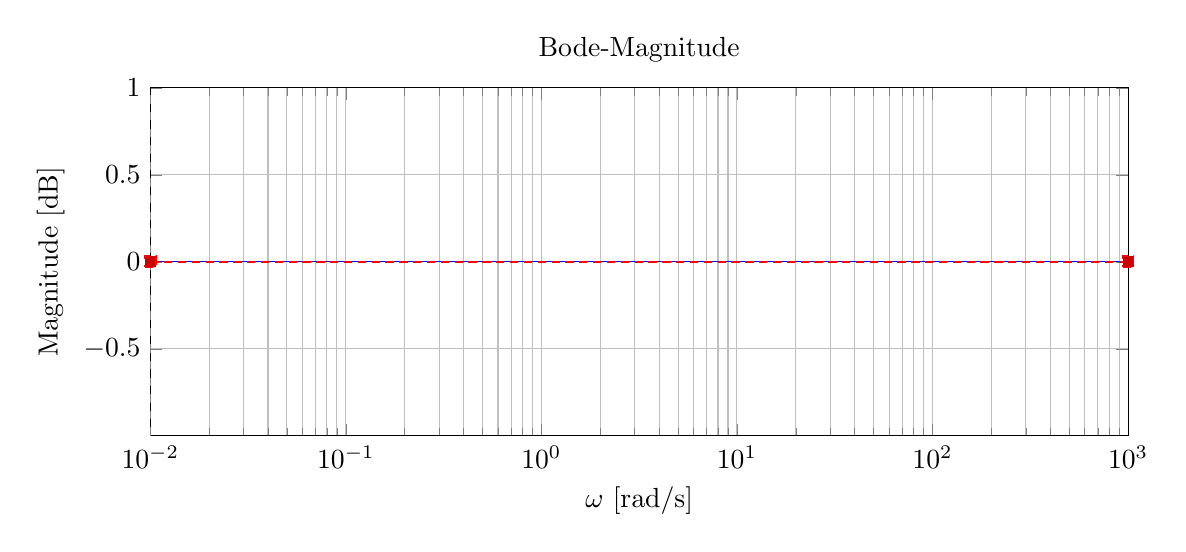
\begin{tikzpicture}
\begin{semilogxaxis}[
  width=14cm,height=6cm,
  xmin=1e-2,xmax=1e3,
  xlabel={$\omega$ [rad/s]},
  ylabel={Magnitude [dB]},
  grid=both,
  title={Bode-Magnitude}
]
\addplot[
  domain=1e-2:1e3,
  samples=2,
  mark=none,
  line width=0.3pt,
  blue
] {0};
\addplot+[domain=1e-2:1e3,samples=2,dashed,dash pattern=on 3pt off 2pt,line width=0.6pt,red] {0};
\draw[gray,dashed] (rel axis cs:0,0) -- (rel axis cs:0,1);
\end{semilogxaxis}
\end{tikzpicture}
\vspace{6mm}
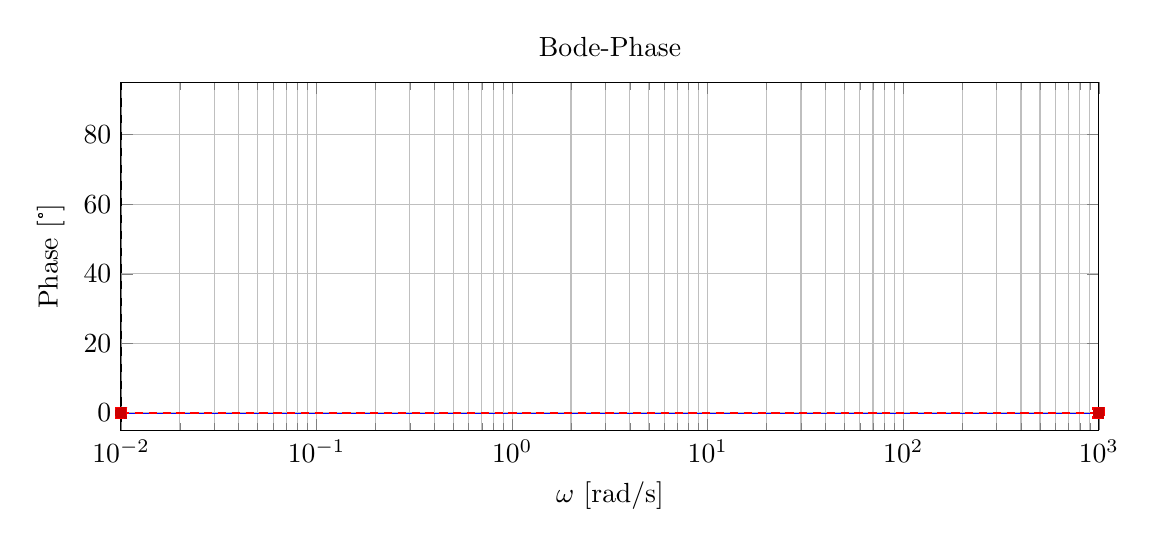
\begin{tikzpicture}
\begin{semilogxaxis}[
  width=14cm,height=6cm,
  xmin=1e-2,xmax=1e3,
  ymin=-5,ymax=95,
  xlabel={$\omega$ [rad/s]},
  ylabel={Phase [°]},
  grid=both,
  title={Bode-Phase}
]
\addplot[
  domain=1e-2:1e3,
  samples=2,
  mark=none,
  line width=0.3pt,
  blue
] {0};
\addplot+[domain=1e-2:1e3,samples=2,dashed,dash pattern=on 3pt off 2pt,line width=0.6pt,red] {0};
\draw[gray,dashed] (rel axis cs:0,0) -- (rel axis cs:0,1);
\end{semilogxaxis}
\end{tikzpicture}
\end{center}
\newpage
\subsection{Erklärung}
\vspace{5mm}
\begin{description}[leftmargin=1.2em,labelsep=.6em,font=\bfseries]
\item[Schritt 1] Kürzung: Zähler und Nenner sind identisch, daher $H(s)\equiv1$. DC-Faktor $1\Rightarrow |H|_{\mathrm{DC}}=0\,\mathrm{dB}$; Anfangssteigung $0\,\mathrm{dB/dec}$; Phase $0^\circ$.
\item[Schritt 2] Keine Ecken: keine endlichen Pole/Nullstellen nach Kürzung, daher keine Eckfrequenzen und keine Übergangsdekaden. Die Geradennäherungen decken sich exakt mit dem exakten Verlauf.
\item[Schritt 3] Grenzverhalten: für $\omega\to0$ und $\omega\to\infty$ bleibt $|H(\j\omega)|=1$ und $\angle H(\j\omega)=0^\circ$; das gesamte Bode-Diagramm ist konstant.
\end{description}

\vspace{0.5cm}
\medskip
\noindent\textbf{Stückweise Näherung}
\[
|H(\j\omega)|_{\mathrm{dB}}\approx
\begin{cases}
0,& \omega\ll1,\\[4pt]
0,& \omega=1,\\[4pt]
0,& \omega\gg1,
\end{cases}
\qquad
\]
\newpage
\section{}
\[
H(s)=\frac{4}{s^2-4}=\frac{4}{(s-2)(s+2)}\,.
\]
\subsection{Bode-Diagramm}
\begin{center}
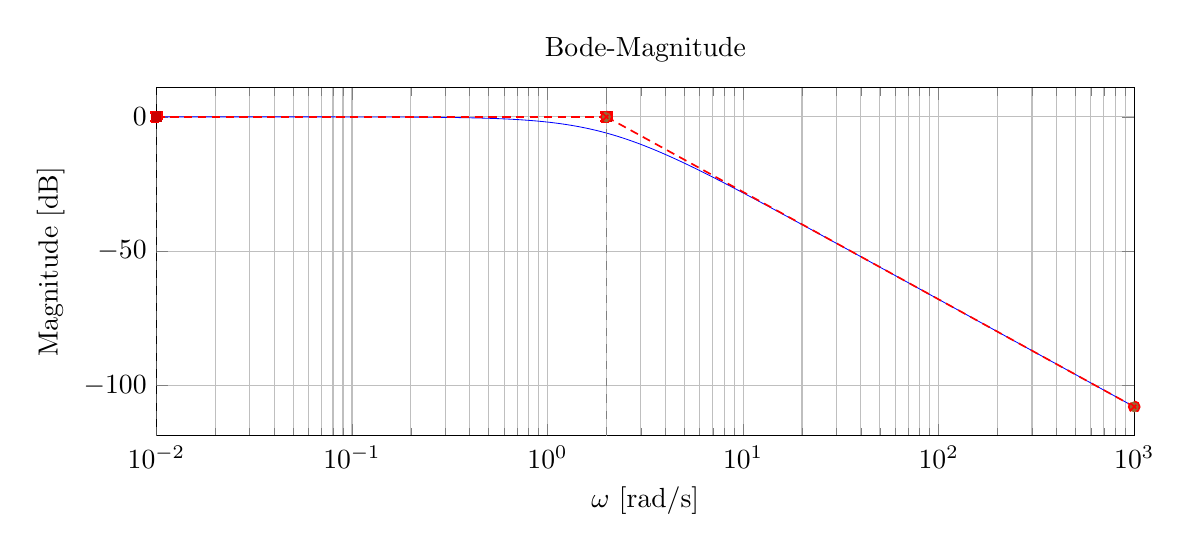
\begin{tikzpicture}
\begin{semilogxaxis}[
  width=14cm,height=6cm,
  xmin=1e-2,xmax=1e3,
  xlabel={$\omega$ [rad/s]},
  ylabel={Magnitude [dB]},
  grid=both,
  title={Bode-Magnitude}
]
\addplot[
  domain=1e-2:1e3,
  samples=800,
  mark=none,
  line width=0.3pt,
  blue
] {-40*ln(sqrt(1 + (x/2)^2))/ln(10)};
\addplot+[domain=1e-2:2,samples=2,dashed,dash pattern=on 3pt off 2pt,line width=0.6pt,red] {0};
\addplot+[domain=2:1e3,samples=2,dashed,dash pattern=on 3pt off 2pt,line width=0.6pt,red] {-40*ln(x/2)/ln(10)};
\draw[gray,dashed] (rel axis cs:0,0) -- (rel axis cs:0,1);
\draw[gray,dashed] (axis cs:2,\pgfkeysvalueof{/pgfplots/ymin}) -- (axis cs:2,\pgfkeysvalueof{/pgfplots/ymax});
\node[gray,anchor=south east] at (axis cs:2,\pgfkeysvalueof{/pgfplots/ymax}) {\scriptsize Pole $\omega_p=2$ (LHP \& RHP)};
\end{semilogxaxis}
\end{tikzpicture}
\vspace{6mm}
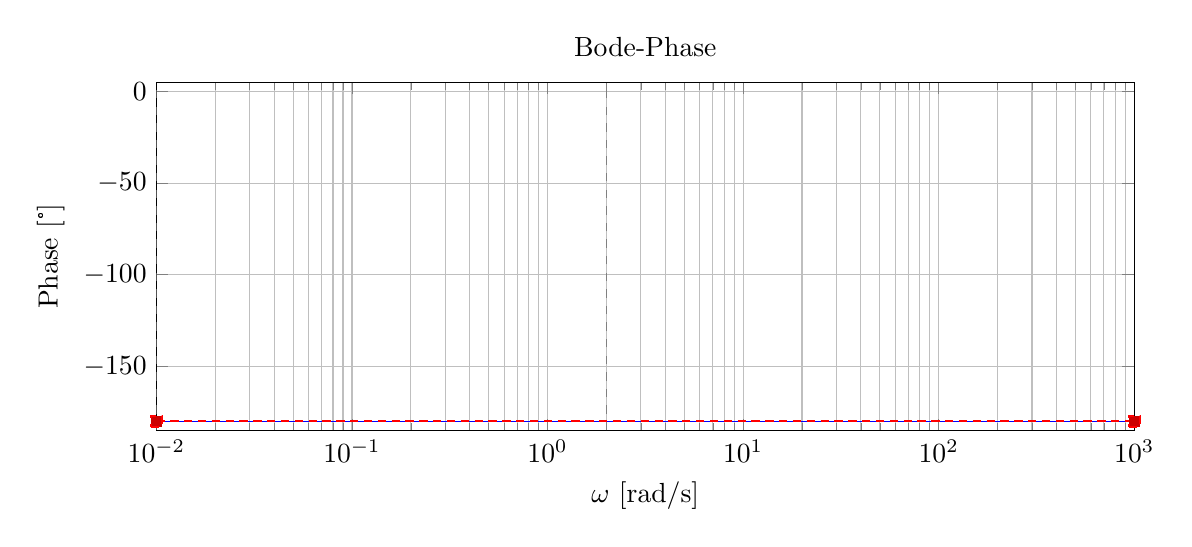
\begin{tikzpicture}
\begin{semilogxaxis}[
  width=14cm,height=6cm,
  xmin=1e-2,xmax=1e3,
  ymin=-185,ymax=5,
  xlabel={$\omega$ [rad/s]},
  ylabel={Phase [°]},
  grid=both,
  title={Bode-Phase}
]
\addplot[
  domain=1e-2:1e3,
  samples=2,
  mark=none,
  line width=0.3pt,
  blue
] {-180};
\addplot+[domain=1e-2:1e3,samples=2,dashed,dash pattern=on 3pt off 2pt,line width=0.6pt,red] {-180};
\draw[gray,dashed] (rel axis cs:0,0) -- (rel axis cs:0,1);
\draw[gray,dashed] (axis cs:2,\pgfkeysvalueof{/pgfplots/ymin}) -- (axis cs:2,\pgfkeysvalueof{/pgfplots/ymax});
\node[gray,anchor=south east] at (axis cs:2,\pgfkeysvalueof{/pgfplots/ymax}) {\scriptsize Pole $\omega_p=2$ (LHP \& RHP)};
\end{semilogxaxis}
\end{tikzpicture}
\end{center}
\newpage
\subsection{Erklärung}
\vspace{5mm}
\begin{description}[leftmargin=1.2em,labelsep=.6em,font=\bfseries]
\item[Schritt 1] Faktorisierung: $H(s)=\dfrac{4}{(s-2)(s+2)}$. DC-Wert $H(0)=-1\Rightarrow |H|_{\mathrm{DC}}=0\,\mathrm{dB}$; das negative Vorzeichen liefert eine konstante Zusatzphase von $-180^\circ$. Anfangssteigung $0\,\mathrm{dB/dec}$.
\item[Schritt 2] Pole bei $\omega_p=2\,\mathrm{rad/s}$ (einer RHP, einer LHP): Magnitudenbeitrag entspricht einem Doppelpol bei $\omega=2$ $\Rightarrow$ ab $\omega=2$ Slope $-40\,\mathrm{dB/dec}$. Am Eckpunkt exakte Dämpfung $-20\log_{10}2\approx-6.02\,\mathrm{dB}$. Phasenverlauf: die variablen Beiträge der LHP- und RHP-Polphase heben sich auf; netto bleibt die Phase für alle $\omega$ konstant $-180^\circ$ (nicht-minimumphasig wegen RHP-Pol).
\item[Schritt 3] Grenzverhalten: für $\omega\ll2$ bleibt $|H(\j\omega)|\approx1$; für $\omega\gg2$ folgt $|H(\j\omega)|_{\mathrm{dB}}\approx-40\log_{10}(\omega/2)$; die Phase bleibt über das gesamte Spektrum bei $-180^\circ$.
\end{description}

\vspace{0.5cm}
\medskip
\noindent\textbf{Stückweise Näherung}
\[
|H(\j\omega)|_{\mathrm{dB}}\approx
\begin{cases}
0,& \omega\ll2,\\[4pt]
-20\log_{10}2,& \omega=2,\\[4pt]
-40\log_{10}(\omega/2),& \omega\gg2,
\end{cases}
\qquad
\]
\newpage
\section{}
\[
H(s)=\frac{-1000\,(s+2)^2}{4\,(s+1)^3\,(s+10)}=-250\,\frac{(s+2)^2}{(s+1)^3\,(s+10)}\,.
\]
\subsection{Bode-Diagramm}
\begin{center}
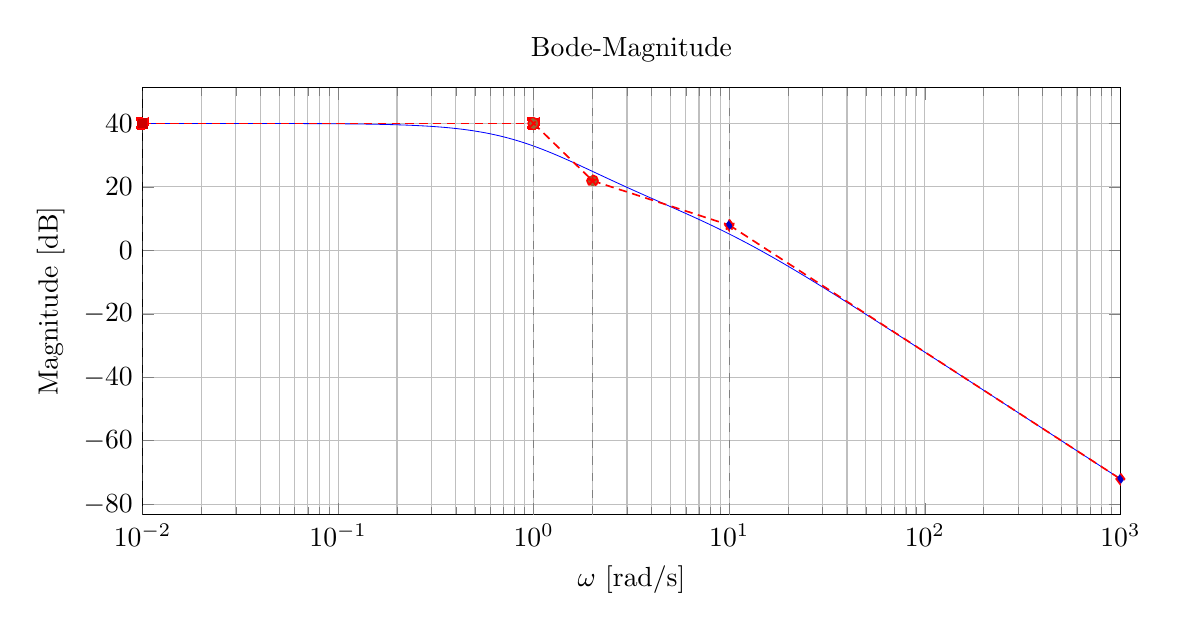
\begin{tikzpicture}
\begin{semilogxaxis}[
  width=14cm,height=7cm,
  ytick distance=20,
  xmin=1e-2,xmax=1e3,
  xlabel={$\omega$ [rad/s]},
  ylabel={Magnitude [dB]},
  grid=both,
  title={Bode-Magnitude}
]
\addplot[
  domain=1e-2:1e3,
  samples=900,
  mark=none,
  line width=0.3pt,
  blue
] {20*ln(250)/ln(10)
    +40*ln(sqrt(4 + x^2))/ln(10)
    -60*ln(sqrt(1 + x^2))/ln(10)
    -20*ln(sqrt(100 + x^2))/ln(10)};
\addplot+[domain=1e-2:1,samples=2,dashed,dash pattern=on 3pt off 2pt,line width=0.6pt,red] {40};
\addplot+[domain=1:2,samples=2,dashed,dash pattern=on 3pt off 2pt,line width=0.6pt,red] {40 - 60*ln(x)/ln(10)};
\addplot+[domain=2:1e1,samples=2,dashed,dash pattern=on 3pt off 2pt,line width=0.6pt,red] {40 - 60*ln(2)/ln(10) - 20*ln(x/2)/ln(10)};
\addplot+[domain=1e1:1e3,samples=2,dashed,dash pattern=on 3pt off 2pt,line width=0.6pt,red] {40 - 60*ln(2)/ln(10) - 20*ln(10/2)/ln(10) - 40*ln(x/10)/ln(10)};
\draw[gray,dashed] (rel axis cs:0,0) -- (rel axis cs:0,1);
\draw[gray,dashed] (axis cs:1,\pgfkeysvalueof{/pgfplots/ymin}) -- (axis cs:1,\pgfkeysvalueof{/pgfplots/ymax});
\draw[gray,dashed] (axis cs:2,\pgfkeysvalueof{/pgfplots/ymin}) -- (axis cs:2,\pgfkeysvalueof{/pgfplots/ymax});
\draw[gray,dashed] (axis cs:10,\pgfkeysvalueof{/pgfplots/ymin}) -- (axis cs:10,\pgfkeysvalueof{/pgfplots/ymax});
\node[gray,anchor=south east] at (axis cs:2,\pgfkeysvalueof{/pgfplots/ymax}) {\scriptsize Nullstelle $\omega_z=2$ (doppelt)};
\node[gray,anchor=south east] at (axis cs:1,\pgfkeysvalueof{/pgfplots/ymax}) {\scriptsize Pol $\omega_p=1$ (dreifach)};
\node[gray,anchor=south east] at (axis cs:10,\pgfkeysvalueof{/pgfplots/ymax}) {\scriptsize Pol $\omega_p=10$};
\end{semilogxaxis}
\end{tikzpicture}
\vspace{6mm}
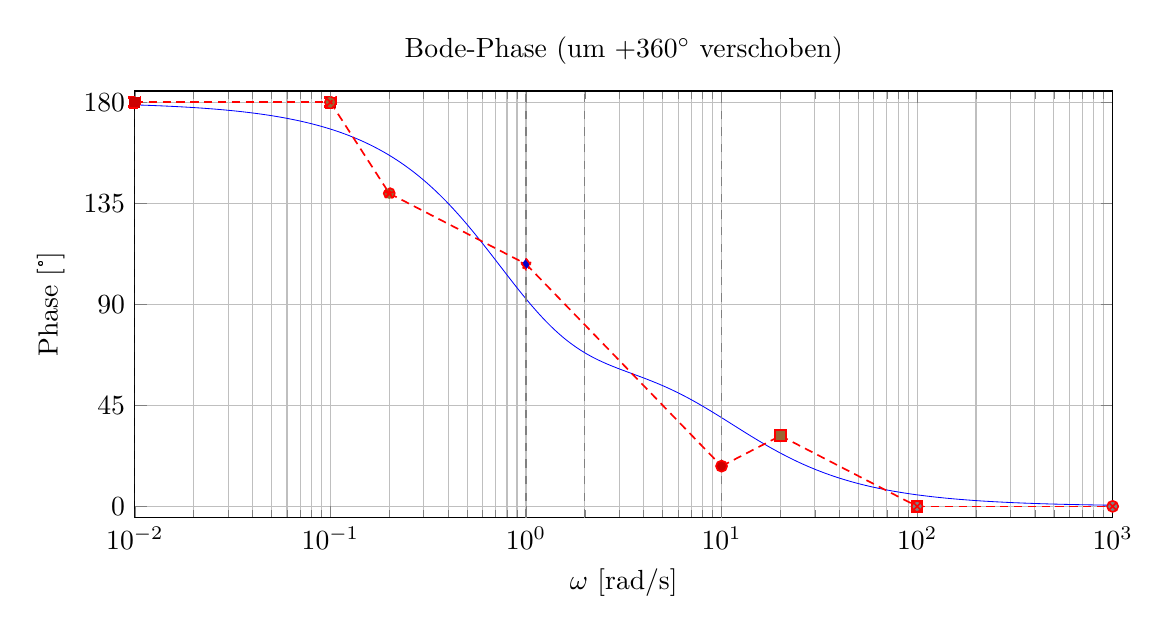
\begin{tikzpicture}
\begin{semilogxaxis}[
  width=14cm,height=7cm,
  xmin=1e-2,xmax=1e3,
  ymin=-5,ymax=185,
  ytick distance=45,
  xlabel={$\omega$ [rad/s]},
  ylabel={Phase [°]},
  grid=both,
  title={Bode-Phase (um $+360^\circ$ verschoben)}
]
% exakte (blaue) Phase: +360° Shift
\addplot[
  domain=1e-2:1e3,
  samples=900,
  mark=none,
  line width=0.3pt,
  blue
] {180 + 2*atan(x/2) - 3*atan(x) - atan(x/10)};

% rote Geradennäherung, korrekt platziert und +360° verschoben
\addplot+[domain=1e-2:1e-1,samples=2,dashed,dash pattern=on 3pt off 2pt,line width=0.6pt,red]{180};
\addplot+[domain=1e-1:2e-1,samples=2,dashed,dash pattern=on 3pt off 2pt,line width=0.6pt,red]{180 - 135*ln(x/0.1)/ln(10)};
\addplot+[domain=2e-1:1e0,samples=2,dashed,dash pattern=on 3pt off 2pt,line width=0.6pt,red]{180 - 135*ln(2)/ln(10) - 45*ln(x/0.2)/ln(10)};
\addplot+[domain=1e0:1e1,samples=2,dashed,dash pattern=on 3pt off 2pt,line width=0.6pt,red]{180 - 135*ln(2)/ln(10) - 45*ln(5)/ln(10) - 90*ln(x)/ln(10)};
\addplot+[domain=1e1:2e1,samples=2,dashed,dash pattern=on 3pt off 2pt,line width=0.6pt,red]{180 - 135*ln(2)/ln(10) - 45*ln(5)/ln(10) - 90 + 45*ln(x/10)/ln(10)};
\addplot+[domain=2e1:1e2,samples=2,dashed,dash pattern=on 3pt off 2pt,line width=0.6pt,red]{180 - 135*ln(2)/ln(10) - 45*ln(5)/ln(10) - 90 + 45*ln(2)/ln(10) - 45*ln(x/20)/ln(10)};
\addplot+[domain=1e2:1e3,samples=2,dashed,dash pattern=on 3pt off 2pt,line width=0.6pt,red]{0};

\draw[gray,dashed] (rel axis cs:0,0) -- (rel axis cs:0,1);
\draw[gray,dashed] (axis cs:1,\pgfkeysvalueof{/pgfplots/ymin}) -- (axis cs:1,\pgfkeysvalueof{/pgfplots/ymax});
\draw[gray,dashed] (axis cs:2,\pgfkeysvalueof{/pgfplots/ymin}) -- (axis cs:2,\pgfkeysvalueof{/pgfplots/ymax});
\draw[gray,dashed] (axis cs:10,\pgfkeysvalueof{/pgfplots/ymin}) -- (axis cs:10,\pgfkeysvalueof{/pgfplots/ymax});
\node[gray,anchor=south east] at (axis cs:2,\pgfkeysvalueof{/pgfplots/ymax}) {\scriptsize Nullstelle $\omega_z=2$ (doppelt)};
\node[gray,anchor=south east] at (axis cs:1,\pgfkeysvalueof{/pgfplots/ymax}) {\scriptsize Pol $\omega_p=1$ (dreifach)};
\node[gray,anchor=south east] at (axis cs:10,\pgfkeysvalueof{/pgfplots/ymax}) {\scriptsize Pol $\omega_p=10$};
\end{semilogxaxis}
\end{tikzpicture}
\end{center}
\newpage
\section{}
\[
H(s)=\frac{2\,s}{s^2+2s+1}=\frac{2\,s}{(s+1)^2}\,.
\]
\subsection{Bode-Diagramm}
\begin{center}
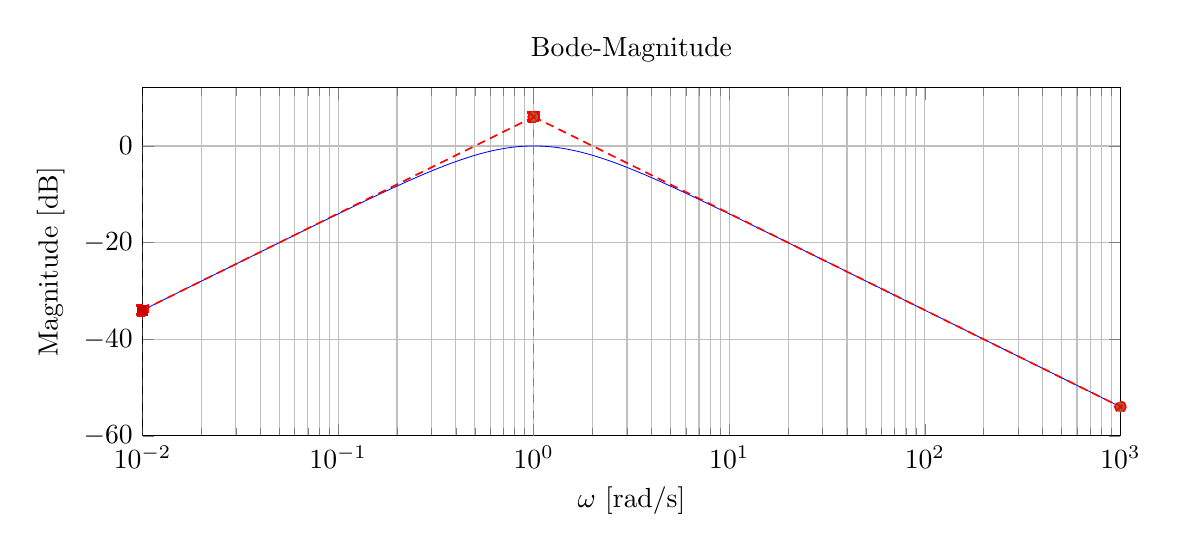
\begin{tikzpicture}
\begin{semilogxaxis}[
  width=14cm,height=6cm,
  xmin=1e-2,xmax=1e3,
  xlabel={$\omega$ [rad/s]},
  ylabel={Magnitude [dB]},
  grid=both,
  title={Bode-Magnitude}
]
\addplot[
  domain=1e-2:1e3,
  samples=700,
  mark=none,
  line width=0.3pt,
  blue
] {20*ln(2)/ln(10) + 20*ln(x)/ln(10) - 40*ln(sqrt(1 + x^2))/ln(10)};
\addplot+[domain=1e-2:1,samples=2,dashed,dash pattern=on 3pt off 2pt,line width=0.6pt,red] {20*ln(2)/ln(10) + 20*ln(x)/ln(10)};
\addplot+[domain=1:1e3,samples=2,dashed,dash pattern=on 3pt off 2pt,line width=0.6pt,red] {20*ln(2)/ln(10) - 20*ln(x)/ln(10)};
\draw[gray,dashed] (rel axis cs:0,0) -- (rel axis cs:0,1);
\draw[gray,dashed] (axis cs:1,\pgfkeysvalueof{/pgfplots/ymin}) -- (axis cs:1,\pgfkeysvalueof{/pgfplots/ymax});
\node[gray,anchor=south east] at (axis cs:1,\pgfkeysvalueof{/pgfplots/ymax}) {\scriptsize Pol $\omega_p=1$ (doppelt)};
\node[gray,anchor=south east] at (axis cs:1e-2,\pgfkeysvalueof{/pgfplots/ymax}) {\scriptsize Nullstelle im Ursprung};
\end{semilogxaxis}
\end{tikzpicture}
\vspace{6mm}
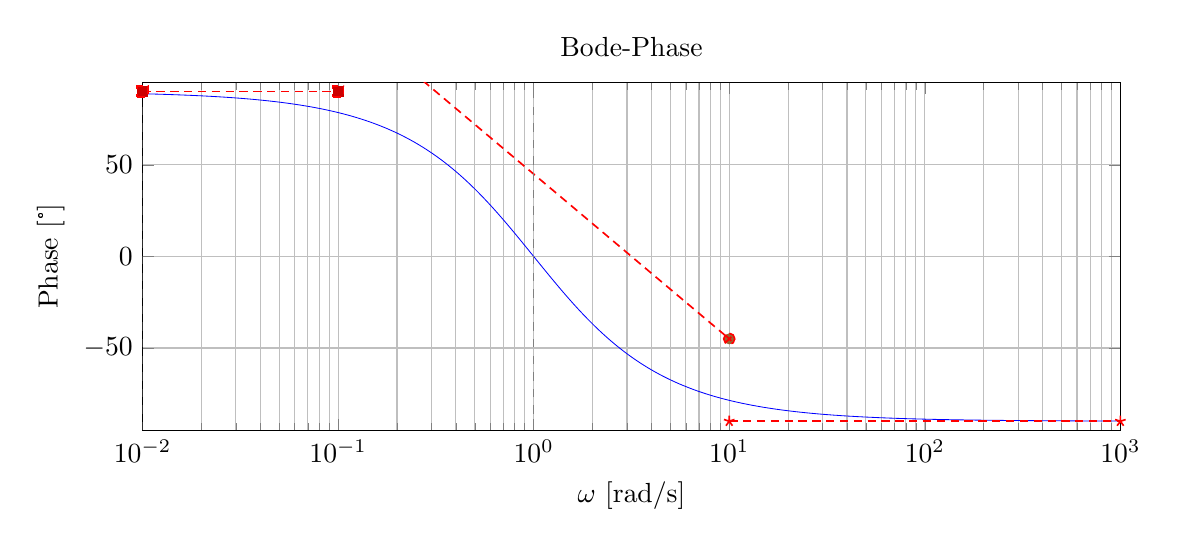
\begin{tikzpicture}
\begin{semilogxaxis}[
  width=14cm,height=6cm,
  xmin=1e-2,xmax=1e3,
  ymin=-95,ymax=95,
  xlabel={$\omega$ [rad/s]},
  ylabel={Phase [°]},
  grid=both,
  title={Bode-Phase}
]
\addplot[
  domain=1e-2:1e3,
  samples=700,
  mark=none,
  line width=0.3pt,
  blue
] {90 - 2*atan(x)};
\addplot+[domain=1e-2:1e-1,samples=2,dashed,dash pattern=on 3pt off 2pt,line width=0.6pt,red] {90};
\addplot+[domain=1e-1:1e1,samples=2,dashed,dash pattern=on 3pt off 2pt,line width=0.6pt,red] {45 - 90*ln(x)/ln(10)};
\addplot+[domain=1e1:1e3,samples=2,dashed,dash pattern=on 3pt off 2pt,line width=0.6pt,red] {-90};
\draw[gray,dashed] (rel axis cs:0,0) -- (rel axis cs:0,1);
\draw[gray,dashed] (axis cs:1,\pgfkeysvalueof{/pgfplots/ymin}) -- (axis cs:1,\pgfkeysvalueof{/pgfplots/ymax});
\node[gray,anchor=south east] at (axis cs:1,\pgfkeysvalueof{/pgfplots/ymax}) {\scriptsize Pol $\omega_p=1$ (doppelt)};
\node[gray,anchor=south east] at (axis cs:1e-2,\pgfkeysvalueof{/pgfplots/ymax}) {\scriptsize Nullstelle im Ursprung};
\end{semilogxaxis}
\end{tikzpicture}
\end{center}
\newpage
\subsection{Erklärung}
\vspace{5mm}
\begin{description}[leftmargin=1.2em,labelsep=.6em,font=\bfseries]
\item[Schritt 1] Nullstelle im Ursprung und Faktor $2$: für $\omega\ll1$ gilt $|H(\j\omega)|\approx 2\,\omega$ $\Rightarrow$ Startsteigung $+20\,\mathrm{dB/dec}$, Startniveau $20\log_{10}2\approx6.02\,\mathrm{dB}$; Startphase $\approx+90^\circ$.
\item[Schritt 2] Doppelter Pol bei $\omega=1\,\mathrm{rad/s}$: ab $\omega=1$ zusätzliche Steigungsänderung um $-40\,\mathrm{dB/dec}$; Netto-Slope für $\omega\gg1$ ist $-20\,\mathrm{dB/dec}$ ($|H|\sim 2/\omega$). Exakt am Eckpunkt: $|H(\j1)|=1\Rightarrow 0\,\mathrm{dB}$, also $20\log_{10}2-20\log_{10}2=0$ relativ zur Geraden. Phasenabfall der beiden Pole zusammen $180^\circ$ über $\omega\in[0.1,10]$; Näherung: $45^\circ-90^\circ\log_{10}\omega$.
\item[Schritt 3] Grenzverhalten: $\omega\ll1\Rightarrow |H|_{\mathrm{dB}}\approx 20\log_{10}2+20\log_{10}\omega$, $\angle H\approx+90^\circ$; $\omega\gg1\Rightarrow |H|_{\mathrm{dB}}\approx 20\log_{10}2-20\log_{10}\omega$, $\angle H\to-90^\circ$.
\end{description}

\vspace{0.5cm}
\medskip
\noindent\textbf{Stückweise Näherung}
\[
|H(\j\omega)|_{\mathrm{dB}}\approx
\begin{cases}
20\log_{10}2+20\log_{10}\omega,& \omega\ll1,\\[4pt]
\left.\;20\log_{10}2\;\right.-20\log_{10}2=0,& \omega=1,\\[4pt]
20\log_{10}2-20\log_{10}\omega,& \omega\gg1,
\end{cases}
\qquad
\]
\newpage
\end{document}
